\chapter{ChromoPainter and ancient DNA}
\label{chapterlabel2}

\section{Introduction}

This chapter is related to the use of ChromoPainter on low coverage ancient DNA samples. 

First, I will describe the existing methodology, ChromoPainterV2, and then a new version I have developed, ChromoPainterUncertainty, which is designed to mitigate bias related to sequencing coverage. 

Next I will perform benchmarking tests on all the steps necessary to analyse low-coverage ancient DNA with ChromoPainter. This includes genotype calling and genotype likelihood estimation with atlas \cite{Link2017}, phasing and genotype imputation with GLIMPSE \cite{rubinacci2021efficient}, ChromoPainter \cite{Lawson2012} analysis (copy-vector estimation and PCA) and SOURCEFIND ancestry component estimation \cite{Chacon-Duque2018}. I will also describe some of the existing issues pertaining to low coverage ancient DNA and several considered mitigation strategies. Finally, I will simulate, using present-day samples, ancient samples with variable degrees of missing SNPs in order to determine whether ancient samples of a particular coverage have enough typed SNPs to retain haplotype information.   

\section{Methods}

\subsection{Description of the ChromoPainter algorithm} \label{sec:ChromopainterDescription}

As discussed in the introduction, ChromoPainter is a method designed to estimate the amount haplotype sharing between individuals \cite{Lawson2012}. In diploid organisms such as humans and dogs, ignoring copy-number-variation, each genetic autosomal of an individual is represented by two haplotypes. As input, ChromoPainter requires each individual's data to be `phased' into these two haplotypes. Phasing refers to the process of determining which alleles along a chromosome were inherited together from the same parent. 

In ChromoPainter, sampled individuals are split into `donor' and `recipient' haplotypes. It employs the widely-used Li and Stephens copying model \cite{Li2003} to model each recipient haplotype as a mosaic of haplotypes observed in the donor panel. Typically (and throughout this thesis) an individual does not act as a donor to themself, e.g.\ one of the individual's two haplotypes can not act as a donor for the other haplotype. Unlike the original Li and Stephens model, which uses the product of approximate conditionals (PAC) likelihoods, ChromoPainter reconstructs each recipient haplotype as a mosaic of \textit{all} other donor haplotypes. Here, the term `copying' can be though of as a genealogical process where haplotypes are reconstructed using the genealogically closest haplotype. 

Suppose we have a particular recipient haplotype, $h*$, which we wish to paint using $j$ donor haplotypes, denoted by $\{h_{1}, ..., h_{j}\}$. $h*$ consists of a sequence of $L$ alleles denoted $\{h*_{1}, ..., h*_{L}\}$, where $h*_{l}$ is the observed allele at site $l$.

The copying model is implemented in the form of a Hidden Markov Model (HMM), with the observed states being the alleles carried by the donor and recipient individuals, and the hidden states being the `nearest-neighbour' haplotype the recipient haplotype copies from. Thus we can define a hidden-state sequence vector $\{Y_{1}, ..., Y_{L}\}$, which corresponds to which of the $j$ donors $h*$ copies from at a given site $l$. The emission probabilities are given as the probability of $h*$ carrying allele $a$, given it copies from haplotype $y_{l}$, and is conditional upon whether, at site $l$,  $h*$ and $y_{l}$ both carry allele $a$ or not:

\begin{equation} \label{eq:cp}
\Pr(h*_{l} = a \mid Y_{l} = y_{l}) =     
	\begin{cases}
		1.0 - \theta & h_{yl} = a \\
		\theta & h_{yl} \neq a 
	\end{cases}       
\end{equation}

where $\theta$ is the probability of a mutation occurring. The mutation probability $\theta$ can be estimated using Watterson's estimator \cite{Watterson1975}, or estimated using an iterative EM algorithm.

The transition probabilities of the HMM, which are the probabilities of a change in the donor being copied when moving from one SNP to another, is guided by a recombination rate map, with higher recombination rates leading to a higher probability of transitioning. Switches between donors are interpreted as changes in ancestral relationships due to historical recombination and modelled as a Poisson process. 

In ChromoPainterV2, the input genetic data comes in the form of phased genotype calls (i.e. \texttt{1|0}). ChromoPainterV2 produces several different output files. The two which most used in this work are those appended with .chunklengths and .chunkcounts. These matrices are also referred to as `coancestry matrices'. In the chunklengths matrix, $cl$, the entry $cl_{d,r}$ gives the total expected proportion of haplotype segments (defined as a contiguous set of SNPs copied from a single donor) that recipient $r$ copies from donor $d$. Thus, higher values of $cl_{d,r}$ indicate that recipient $r$ and donor $d$ share more recent ancestry. The .chunkcounts matrix instead gives the total number of haplotype segments that recipient $r$ copies from donor $d$.

In this work, `copyvector' is used to refer to the vector of chunklengths that a single recipient individual copies from all donors, or a single row of the coancestry matrix. Throughout, I often define donors as populations, so that{ each element of the copy vector is the total amount of DNA that the recipient matches to all individuals from a given donor population.

\subsubsection{Description of ChromoPainterV2Uncertainty} \label{sec:DescriptionChromoPainterV2Uncertainty}

ChromoPainterUncertainty works in a very similar way to ChromoPainterV2, bar two differences. Firstly, the input data is in the form of an allele probability $0 \leq x \leq 1$, which is given as the probability of observing the alternate allele at that SNP. This value is calculated from the posterior likelihood that an allele has been imputed correctly. This is different to ChromoPainterV2, which uses `hard' allele calls that only take a value of 0 or 1.

Here, I will show how it is possible to incorporate the uncertainty in imputed genotype calls into the ChromoPainter input. Consider the following example: we have a phased genotype in the form \texttt{0|1}, corresponding to the reference allele on the first haplotype and the alternative allele at the second haplotype. I define $G$ as the sum of the genotypes at a SNP; in this case $G=0+1=1$. As GLIMPSE, the imputation and phasing algorithm I will use for this work, provides hard genotype calls, $G$ can be calculated directly.

We also have a posterior genotype likelihood, in the form $GL(p_{0}, p_{1}, p_{2})$, where $p_i$ is the posterior probabilities that the true genotype is $i$. Genotype probability dosage, $D$, is the expected total number of copies of the alternate allele given $GL$. $D$ can be calculated as $p_{1} + [2*p_{2}]$. We can calculate $U$, the uncertainty as $U = |G-D|$. Then, we can assign a probability to each allele; if the allele is \texttt{1} then the allele likelihood is simply $1 - U$ and if the allele is \texttt{0} then the allele likelihood is $0 + U$. Therefore, when there is no uncertainty in the genotype call, the allele probability will be either 0 or 1. When there is uncertainty, the allele probability will take a value $0 \leq x \leq 1$, with more uncertain genotypes tending towards allele probabilities of 0.5. 
                 
The second difference is the incorporation of the allele probability into the emission probability of the HMM. As before, consider a donor $d$ and recipient $r$ at SNP $p$. Now we let $r_x$ be the probability that the recipient haploid $r$ carries the alternative allele, with $d_x$ the probability the donor haploid carries the alternative allele.

\begin{equation} \label{eq:cp_uncertainty}
\Pr(h*_{l} = a \mid Y_{l} = y_{l}) =     
	\begin{cases}
		[1.0 - \theta]  & h_{yl} = a \\
		\theta & h_{yl} \neq a 
	\end{cases}       
\end{equation}

Note that \ref{eq:cp_uncertainty} reduces \ref{eq:cp} if $d_{x} = \{0,1\}$ and if $r_{x} = \{0,1\}$, i.e\ there is no uncertainty in the calls.


\subsection{Generation of downsampled genomes}

I created a set of `downsampled' ancient genomes in order to explicitly quantify the effect of coverage on each stage of the ChromoPainter analysis. I took five high coverage genomes and for each, removed a random subset of reads from the \texttt{.bam} file in order to reduce the coverage to a target level. I then performed each stage of a typical ChromoPainter analysis, e.g.\ mimicking the analyses of new ancient DNA samples I describe in chapters 4 and 5, on the full coverage and downsampled genomes. I also processed a set of X ancient samples from the literature, downloaded from the European Nucleotide Archive, in an identical way to act as comparison samples. 

Five high coverage ancient genomes were downloaded in the form of aligned \texttt{.bam} files from the European Nucleotide Archive:

\begin{enumerate}
\item Yamnaya -- Yamnaya Bronze Age steppe-pastoralist \cite{deBarrosDamgaardeaar7711}
\item UstIshim -- Siberian Upper Palaeolithic hunter-gatherer \cite{Fu2014}
\item sf12 -- Scandinavian Hunter-Gatherer \cite{Gunther2018a}
\item LBK -- early European farmer from the \textit{Linearbandkeramik} culture from Stuttgart, Germany \cite{Lazaridis2014}
\item Loschbour -- 8,000 year-old hunter-gatherer from Luxembourg) \cite{Lazaridis2014}
\end{enumerate}

These samples were chosen due to their high original coverage ($>18$x), and because they represent some of the ancestries present in Western Eurasia over the past 40,000 years.  

For each full coverage, downsampled and literature ancient \texttt{.bam} file was processed using the atlas (version 1.0, commit f612f28) pipeline \cite{Link2017} \\(\url{https://bitbucket.org/wegmannlab/atlas/wiki/Home}). First, the validity of each file was assessed (i.e. ensuring that each \texttt{.bam} file was not malformed in any way) using ValidateSamFile command from PicardTools \cite{Picard2018toolkit}. atlas is a suite of software designed for processing low-coverage ancient DNA and was chosen following the recommendation of Hui et al (2020) \cite{hui2020evaluating}, as it explicitly accounts for post-mortem damage (PMD) patterns in ancient DNA. The most common form of PMD is C-deamination, which leads to a C->T transition on the affected strand and a G-->A transition on the complimentary strand.

I then downsampled each full-coverage genome using the \texttt{atlas downsample} task, resulting in a \texttt{.bam} file with coverages 0.1x, 0.5x, 0.8x, 1x, 2x, 3.5x, 5x, 10x and 20x per individual. 

Again, for each full coverage, downsampled and literature ancient \texttt{.bam} file, I estimated post-mortem damage (PMD) patterns using the \texttt{atlas estimatePMD} task. Recalibration parameters were then estimated using the atlas \texttt{atlas recal} task. Finally, both the recalibration and PMD parameters were given to the \texttt{atlas callNEW} task which produces genotype calls and genotype likelihood estimates for each downsampled and full coverage \texttt{.bam}. For this stage, I made calls at the 77,818,264 genome-wide positions present in the phase 3 thousand genomes project \cite{1000GenomesProjectConsortium2015}. This was done to reduce the risk of calling false-positive (i.e.\ falsely polymorphic) genotypes in the aDNA samples. No minimum read-depth filter was applied when calling genotypes. This step resulted in a \texttt{.vcf} file for each of the X samples. For each of the 22 autosomes, I merged all X samples together into a single \texttt{.vcf} file. 

atlas does not make calls at positions in the genome where no reads have been aligned. If multiple \texttt{.vcf} files are merged together, and at a given position in the genome, some samples contain genotype calls and others do not, this position will be present but the genotype will be set as missing \texttt{./.} in  the merged \texttt{.vcf}. Therefore, the merged \texttt{.vcf} contained positions at all 77,818,264 positions, as across all X samples, at least one individual have a genotype call at each position. 

\subsection{Generation of ancient literature samples} \label{AncientReferenceSamples}

I also generated a set of ancient samples from the literature to use as donors in the ChromoPainter analysis.

This dataset consists of 918 other ancient samples from the literature given in Appendix section \ref{section:AncientReferenceDataset}. These samples were of variable coverage, ranging from 0.002-72x coverage, and chosen because of their previously reported relevance to understanding past ancestry patterns in European populations like those analysed in chapters 4 and 5. These 918 consist of all samples given in Table \ref{tab:AncientReferenceDataset} were processed in an identical way to the downsampled target individuals described in the previous section, other than they were not downsampled.  

\subsection{Imputation and phasing - GLIMPSE}

Genotype imputation and phasing are two important steps for processing low-coverage ancient DNA. Low coverage ($<$1x) samples typically lack enough read information to make accurate genotype calls at most positions in the genome, and often do not contain any reads at many positions \cite{nielsen2011genotype}. Therefore, it can be helpful to use external information from a high-coverage reference panel in order to improve the accuracy of genotype calls and phasing, reducing the impact of errors on downstream analyses \cite{rubinacci2021efficient}. 

Three different characteristics are desirable for an imputation algorithm in this context. Firstly, it should take genotype likelihoods as input. This is because genotype likelihoods allow for flexible representation of the possible genotypes at a particular position, particularly when there may not be enough coverage to make a hard genotype call. Secondly, it should emit posterior genotype-probabilities which, when accurately calibrated, give the probability that a particular genotype call is correct. This is necessary for estimating the uncertainty values, described in section \ref{sec:DescriptionChromoPainterV2Uncertainty}, needed for ChromoPainterUncertainty analysis. Thirdly, the algorithm must be able to complete in a reasonable running time when using a large number of samples and high number of SNPs. Using a large number of densely positioned SNPs (e.g. such as the approximately 77 million identified in the 1000 Genomes Project) increases the useful linkage-disequilibrium information between each SNP, and it is well-established that increasing the number of individuals used in imputation/phasing reference panels improves accuracy \cite{delaneau2018integrative, HUANG2009235, mccarthy2016reference, rubinacci2021efficient}. 

Two programs, Beagle 4.0 \cite{Browning2007} and GLIMPSE \cite{rubinacci2021efficient} fulfil the first and second criteria above, but GLIMPSE offers up to 1000x reduction in running time compared to Beagle 4.0 \cite{rubinacci2021efficicanent}, and hence chose it for the imputation and phasing steps.   

Phasing and imputation ideally requires a reference panel of high-coverage present-day individuals. I used the 1000 Genomes Project dataset re-sequenced to 30x average coverage, which contains 3202 individuals from 26 worldwide populations \cite{byrska2021high}. A description of the processing of this reference dataset can be found in Appendix \ref{section:1000genomes}.

I merged together i) the full coverage individuals, ii) downsampled individuals and iii) 918 ancient samples from the literature into a single bcf file using bcftools (version 1.11-60-g09dca3e) \cite{li2011statistical} to act as the samples for GLIMPSE to phase. Here, `target' refers to the individuals being imputed/phased and `reference' refers to the reference panel.  

Following the GLIMPSE tutorial (\url{https://odelaneau.github.io/GLIMPSE/tutorial_b38.html}), I first used \texttt{GLIMPSE\_chunk} to split up each  chromosome into chunks, keeping both \texttt{--window-size} and \texttt{--buffer-size} to 2,000,000 base pairs, which is their default settings. I used the b37 genetic map supplied by GLIMPSE for the \texttt{--map} argument. Across all chromosomes, this produced 936 chunks that are on average 2.99Mb long. 

GLIMPSE then imputed each chunk separately, using \texttt{GLIMPSE\_phase} using the same 1000 genomes dataset as a reference and default settings. This stage both imputes missing genotypes and generates a set of haplotype pairs which can be sampled from in a later step to produce phased haplotypes. \texttt{GLIMPSE\_ligate} then merges the imputed chunks back to form single chromosomes using the default settings. I then used \texttt{GLIMPSE\_sample} to produce a .vcf with phased haplotypes sampled for each individual, again using default settings. Consequently, the output of GLIMPSE is i) unphased genotype calls with posterior genotype likelihoods and ii) phased haplotypes.

It is important to note that GLIMPSE leverages information from individuals that have been imputed, `absorbing' them into the reference panel. For example, if there were 100 target samples and 1000 reference samples, each target is phased in turn and then absorbed into the reference panel, so that there would be 1001 reference samples when the second target individual is imputed. This makes it necessary to avoid including the same sample, downsampled to different coverages, in the same set of targets for one imputation run, in order to avoid the confounding effect of allowing an individual to act as the reference to itself. For example, including Loschbour at 0.1x and 10x coverage could mean it imputed itself, a situation which would never occur in reality. 


\subsection{Estimating imputation sensitivity and specificity}

I used rtg-tools-3.11 \cite{cleary2014joint} and the \texttt{vcfeval} task to estimate the sensitivity and specificity of imputation in the downsampled individuals. Here, `baseline' (i.e. the truthset) is defined as the genotype calls in the full coverage individual and the `calls' as the genotype calls in the downsampled individual. Sensitivity and precision are defined as: 

\begin{equation}
sensitivity = \frac{V_{call}-FP}{V_{call}}
\end{equation}

\begin{equation}
precision = \frac{V_{baseline}-FN}{V_{baseline}}
\end{equation}

A `variant' is considered to be a SNP with a genotype that is either \texttt{0/1} or \texttt{1/1}, with $V_{baseline}$ and $V_{call}$ the number of variants called in the full coverage and downsampled genomes, respectively. False negatives (FN) are where a variant is called in the full coverage genome but not in the downsampled genome. False positives (FP) are cases where a variant is called in the downsampled genome but not in the full-coverage genome.

$V$, or true-positive, is the number of events where a variant position (i.e. a SNP with a genotype that is either \texttt{0/1} or \texttt{1/1}) is detected in either the full coverage ($V_{baseline}$) or downsampled ($V_{baseline}$) sample. $FN$ is the number of times that a variant position is called in the full coverage sample and not the downsampled sample. Conversely, $FP$ is the number of times a variant position is called in the downsampled sample and where the same SNP in the full coverage sample is invariant (i.e. \texttt{0/0}). Only genotypes called in the full coverage and downsampled individuals were considered. No allele frequency filters were applied before conducting this analysis.


\subsection{ChromoPainter analysis} \label{ChromoPainter_analysis}

It is important to understand the effect of sequencing coverage on the accuracy of ChromoPainter copyvector estimation. A `copyvector', $c_{r}$, is a vector of length $D$, where each entry gives the total length of genome that recipient individual $r$ most closely matches to each of the $D$ donor individual/populations. I sometimes refer to `normalised' copyvectors; this simply refers to where each entry of $c_r$ is divided by the sum of all entries, scaling the copyvector to sum to 1. 

I painted each downsampled and full coverage ancient individual using a set of 124 ancient individuals, hereafter referred to as the `standard set', selected because they had a sequencing depth greater than 2x. I compared the copyvectors for the same individual at each level of downsampling, to the same individual at full coverage. For example, I compared the copyvector of Yamnaya at 0.1x to the copyvector of the same Yamnaya sample at full coverage. A high correspondence, measured by r-squared for example, between the copyvectors of the full coverage and downsampled individual suggests less effect of coverage. 

To prepare the data for ChromoPainter, I merged the .vcf containing the posterior genotype likelihoods of i) downsampled, ii) full coverage and iii) 124 ancient samples from the literature together, and did the same for the .vcfs containing the phased haplotypes.  I combined the posterior genotype likelihoods with the phased alleles to generate allele likelihoods (described in section \ref{sec:DescriptionChromoPainterV2Uncertainty}) in ChromoPainter-uncertainty format, in addition to per-position recombination rate files. This was performed for each chromosome in turn using my own script (\url{https://github.com/sahwa/vcf_to_ChromoPainter}).

I next used ChromoPainterUncertainty to perform the painting. I assigned the standard set individuals as donors and all downsampled, full coverage and standard set as recipients. The `standard set' samples from the literature were included in order so that they can be used a surrogates in later SOURCEFIND analysis.

I also performed an identical analysis, but using ChromoPainterV2 and hard genotype calls. 

This painting produced a chunklengths matrix for each chromosome which were merged using chromocombine-0.0.4 (\url{https://people.maths.bris.ac.uk/~madjl/finestructure-old/chromocombine.html}). The resulting chunklengths matrix thus gives the total length of genome in centimorgans that a recipient most closely matches to each donor individual. 

\subsection{ChromoPainter Principle Component Analysis}

Principle Component Analysis (PCA) can be used to reduce the underlying structure in the chunklengths coancestry matrix to two dimensions, thus allowing it to be more easily visualised. As individuals cannot paint themselves, the diagonals of each coancestry matrix contain zeros. Therefore, I performed PCA using the fineSTRUCTURE library \url{https://people.maths.bris.ac.uk/~madjl/finestructure/finestructureR.html}.

All downsampled and full coverage individuals were projected onto the principle components of the reference ancient samples. 


\subsection{SOURCEFIND}

The chunklengths coancestry matrix produced by ChromoPainter contains information about the estimated length of genome a recipient most closely matches a given donor individual or population. However, incomplete lineage sorting, where alleles segregate in a way that is discordant to the true phylogeny reflecting the orders in which populations split from one another, means that there are regions in the genome where a recipient individual most closely matches a reference individual that is not from their own population. For example, an individual from France copies non-zero amounts from African donors, despite not having any African ancestry through recent admixture. Furthermore, unequal donor population sizes may bias the aggregated amount copied to a given population. 

Therefore, to account for these issues when estimating ancestry proportions, it is necessary to run an additional step, SOURCEFIND \cite{Chacon-Duque2018}. Simulations have shown that SOURCEFIND ancestry proportions correspond well to simulated truth-set values \cite{Chacon-Duque2018}. The ancestry proportions produced by SOURCEFIND should be interpreted as the proportion of ancestry that each individual/population shares most recently with each surrogate. This need not necessarily imply an admixture event; for instance, you might expect $France$ to have ancestry recently related to both $Germany$ and $Spain$ due to isolation-by-distance rather than admixture. 

SOURCEFIND models each target copyvector as a linear mixture of copyvectors from a set of surrogate groups, inferring the proportion of ancestry for which the target individual is most recently related to each surrogate group. The parameter space of surrogate ancestry proportions is explored using a Markov chain Monte Carlo algorithm, where the ancestry proportions are updated using a Metropolis-Hastings step. The output of SOURCEFIND for each target individual is therefore an $n*p$ matrix, where $n$ is the number of MCMC samples and $p$ is the total number of surrogate groups. 

To test for the effect of coverage on the proportions estimated by SOURCEFIND, I performed two separate analyses, both using the downsampled and full coverage individuals as targets. The first uses three surrogate populations (Yamnaya, Western Hunter-Gatherer and Anatolia Neolithic Farmer), and the second uses an expanded list of 37 surrogate populations. I chose the first set of three surrogates, as these are typically used in ancient DNA analysis to obtain a 'broad' overview of the ancestry of a European individual, as it has been shown that central Europeans within the last 10,000 years can be well modelled as a mixture of those three groups \cite{Lazaridis2014, Haak2015}. Note, this does not mean that there was not admixture from other sources, but that a majority of ancestry of ancient central Europeans can be derived from these sources. This stands to act as a relatively straightforward test case, since the three populations are highly genetically differentiated from one another.

For all runs of SOURCEFIND, I used 1,000,000 iterations, of which 50,000 were designated as burn-ins, and then samples were taken every 50 iterations. 2,000,000 iterations were chosen because my previous tests show that is the minimum necessary to provide reasonably confidence of convergence within reasonable running time (Appendix section \ref{sec:SF_test_iterations}). The rest of the parameters were left as default. Ancestry proportions and credible intervals group were estimated using the CODA R library \cite{oro22547}.

\section{Pre-post GLIMPSE and linked/unlinked PCA test}

I wanted to determine at what stage of the analysis pipeline low coverage samples (0.1x) significantly diverge from the other downsamples when plotted on a PCA. I will hereafter refer to this phenomenom as `coverage-related bias'. For instance, it may be that the coverage-related bias is introduced in the imputation stage. Coverage-related bias can be measured by calculating $d = \sqrt{(PC1_{f} - PC1_{d})^2 + (PC2_{f} - PC2_{d})^2}$, where $(PC1_{f}$ is the PC1 value for the full coverage individual and $(PC1_{d}$ is the equivalent for the downsampled individual. In other words, $d$ measures the Cartesian distance between the full coverage and downsampled individual on principle component space, with higher distances corresponding to more coverage-related bias. 

To test this, I performed a set four PCAs on all downsampled and equivalent full coverage samples and a set of present-day individuals shown in Table \ref{tab:HB_pops}.

For both the ChromoPainter PCAs, in order to account for the zeros on the diagonals of each coancestry matrix, I used the fineSTRUCTURE R library \url{https://people.maths.bris.ac.uk/~madjl/finestructure/finestructureR.html}.

The four PCAs were as follows:

\begin{enumerate}
\item \textbf{Pre-GLIMPSE} Using the genotypes generated by atlas, but before imputation with GLIMPSE, I projected all downsampled ancients of all coverages onto the present-day populations using the eigenstrat library. \cite{Price2006}.
\item \textbf{Post-GLIMPSE} Using the GLIMPSE generated imputed genotypes generated by atlas, I projected all downsampled ancients of all coverages onto the present-day populations using the eigenstrat library.
\item \textbf{ChromoPainter - unlinked} I performed an `all-v-all' unlinked ChromoPainter painting, using all populations in Table \ref{tab:HB_pops}. 
\item \textbf{ChromoPainter - linked} I performed an `all-v-all' unlinked ChromoPainter painting, using all populations in Table \ref{tab:HB_pops}.
\end{enumerate}

Coverage-related bias present in PCA (2) but not (1) indicates it has been introduced in the imputation stage. Similarly, coverage-related bias present in (4) but not (3) suggests that including linkage information introduces bias in low coverage samples. 


\begin{table}
\centering
\begin{tabular}[t]{lc}
\toprule
Population & \thead{Number of\\ samples}\\
\midrule
HB:croatian & 19\\
HB:cypriot & 12\\
HB:french & 28\\
HB:german & 30\\
HB:germanyaustria & 4\\
HB:greek & 20\\
HB:hungarian & 19\\
HB:irish & 7\\
HB:lithuanian & 10\\
HB:mordovian & 15\\
HB:northitalian & 12\\
HB:norwegian & 18\\
HB:polish & 17\\
HB:romanian & 16\\
HB:scottish & 6\\
HB:siciliane & 10\\
HB:southitalian & 18\\
HB:spanish & 34\\
HB:tsi & 98\\
HB:tuscan & 8\\
HB:welsh & 4\\
HB:westsicilian & 10\\
\bottomrule
\end{tabular}
\caption{Population labels and sample sizes of populations included in the pre-post GLIMPSE and linked/unlinked PCA test. All samples are from the Hellenthal and Busby dataset, described in \ref{section:MSPOBIHellBus}.}
\label{tab:HB_pops}
\end{table}


\section{Reducing SNP count} \label{sec:ReducingSNPcount}

One way to mitigate coverage-related bias would be to exclude imputed SNPs which have a low probability of being imputed correctly or restricting analysis to non-imputed SNPs above a certain coverage.

However, reducing the total number and or density of SNPs used in a painting may reduce the accuracy of the estimated copyvectors. All other things being equal, there is less linkage information between two SNPs which are separated by a larger genetic distance. Therefore, it is necessary to precisely determine what effect reducing the number of SNPs has. In particular, we would like to know the minimum number and density of SNPs required to retain the advantages of haplotype-based methods over unlinked methods. 

Using data from the People of the British Isles (POBI) project, previous work showed it is possible to distinguish between British individuals from neighbouring counties Devon and Cornwall using the fineSTRUCTURE algorithm, but not using unlinked methods (ADMIXTURE \cite{alexander2009fast}) \cite{Leslie2015}. Therefore, determining whether it is possible to distinguish between individuals from Devon and Cornwall acts as a good test case for reducing SNPs. In particular I tested how many SNPs can we remove before we lose the ability to distinguish between these two populations.


The original POBI dataset contains 2039 individuals from 33 populations from across England, Northern Ireland, Wales and Scotland, genotyped at 452 592 SNPs. Details of the data preparation for this dataset can be found in Appendix section \ref{section:MSPOBIHellBus}.

Using the \texttt{shuf} unix command, I randomly reduced the total number of SNPs down to only the following percentages: 0.2\%, 1\%, 2\%, 3\%, 4\%, 5\%, 6\%, 7\%, 8\%, 9\%, 10\%, 20\%, 30\%, 40\%, 50\%, 60\%, 70\%, 80\%, 90\%. SNPs were removed from the .vcf files using \texttt{bcftools --view}.

For each target level of reduced SNPs, I painted all individuals from Devon and Cornwall using a `leave-one-out' approach. I then combined the resulting chunklengths matrices across all chromosomes and combined copyvectors columns by donor group, so that each individual was represented by a $K$-vector of values, with element $k$ denoting the proportion of DNA that person matched to any haploid in donor group $k$.

\section{Direct imputation test}

To explicitly test the effect of imputation on the copyvectors estimated by ChromoPainter, I created a dataset which simulated a typical imputation scenario; imputing SNPs after merging two datasets with a low SNP overlap. In particular I did this in a way to mimic a real analysis on ancient samples of approximately 0.15 coverage (determined from empirical data), which have approximately 70,000 SNPs out of 500,000 covered by at least a single read. 

I took the Human Origins dataset (described in Appendix section \ref{HumanOriginsAppendix}), containing 560,240 bi-allelic SNPs and submitted the reduced dataset to the Sanger Imputation Service (\url{https://www.sanger.ac.uk/tool/sanger-imputation-service/}). The Sanger Imputation Service uses Eagle2 \cite{loh2016reference} and the Haplotype Reference Consortium as a reference to impute missing variants. Once the data had been imputed, I subsetted the data back to the original set of 560,240 SNPs. I therefore had a dataset which contained 70,000 non-imputed SNPs and 490,240 imputed SNPs. This is hereafter referred to as the `imputed dataset'. 70,000 non-imputed SNPs was chosen because that is the number of SNPs which overlap between two datasets in Chapter 3 and thus represents a realistic case-study. 

For both the imputed dataset and original Human Origins dataset, I performed an all-v-all painting and combined data across chromosomes. An `all-v-all' painting is where each individual is painted in turn by all other individuals, resulting in an $n$-by-$n$ coancestry matrix, where $n$ is the number of individuals analysed.


\section{Results}

\subsection{Imputation accuracy}

To estimate how accurately GLIMPSE imputes genotypes in ancient samples of differing coverages, I estimated the sensitivity (Fig. \ref{fig:Sensitivity_downsampled_rtgtools}) and precision (Fig.  \ref{fig:precision_downsampled_rtgtools}) of genotype imputation using rtg-tools \cite{cleary2014joint}. This approach compares genotype calls at each position in each downsampled individual after imputation to the same individual at full coverage without imputation.

\begin{figure}[htp]
    \centering
    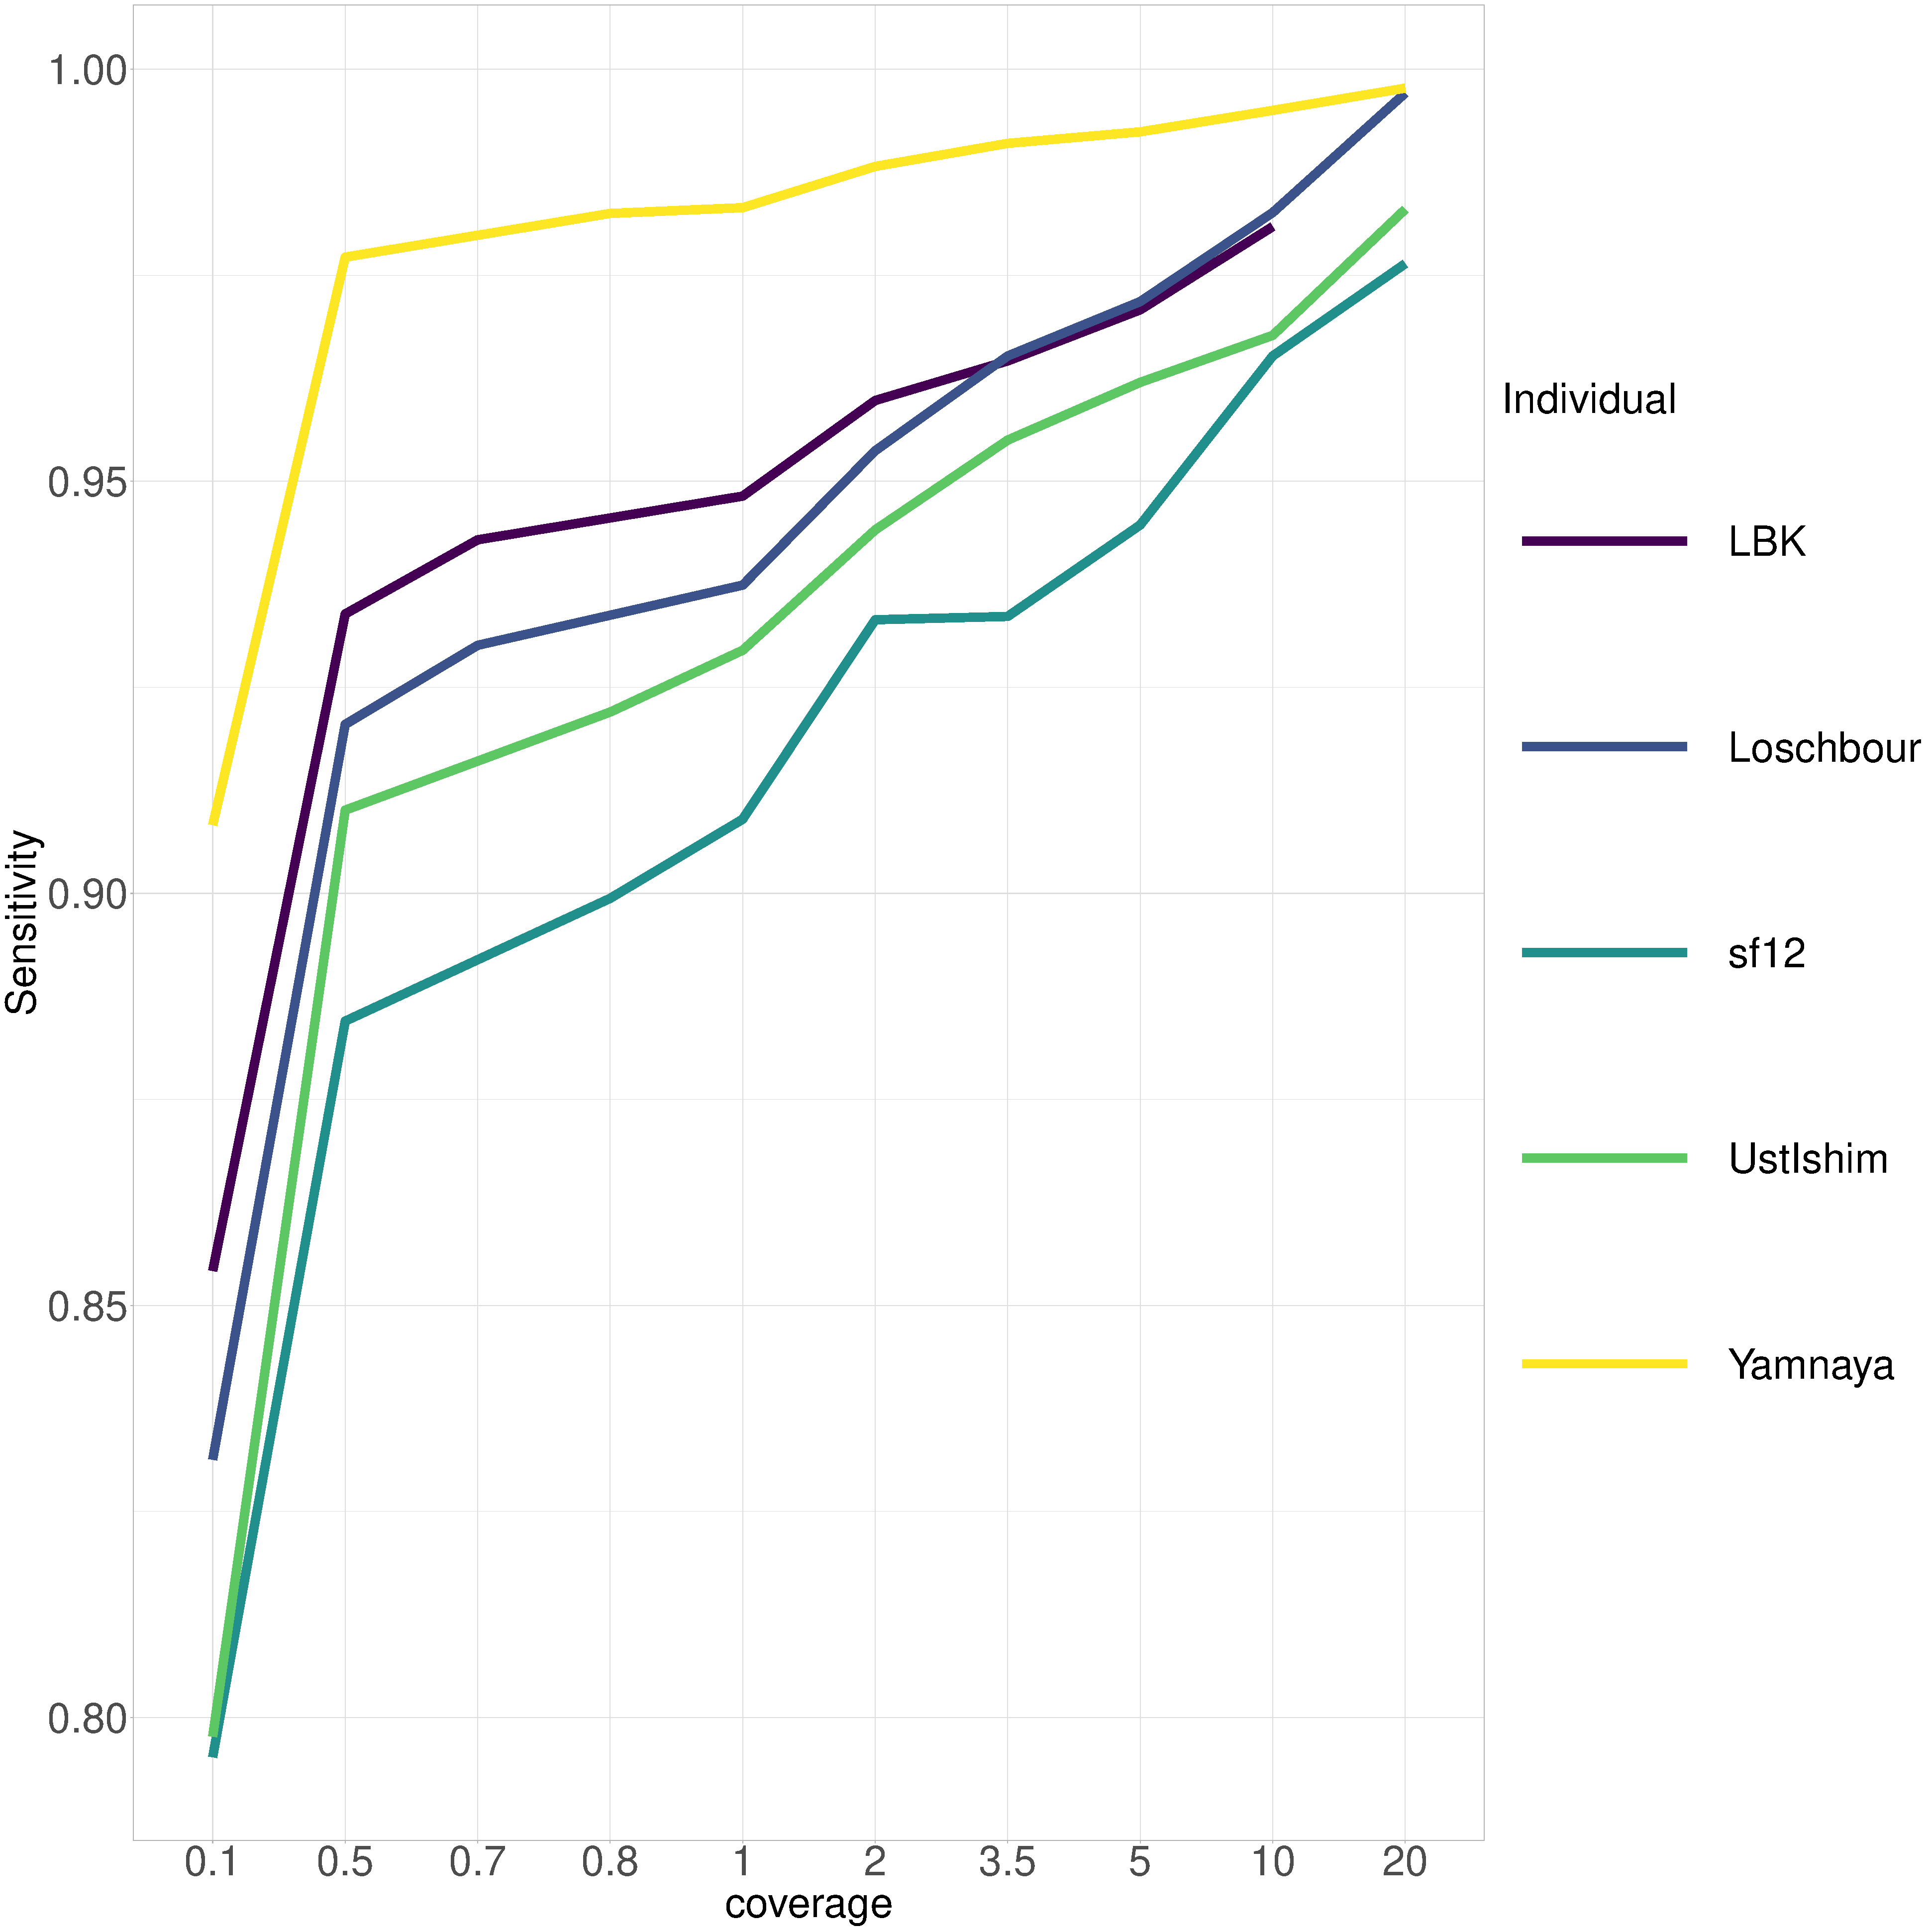
\includegraphics[width=1.0\textwidth]{../images/chapter1/allDownsampled_rtgtools_sensitivity.pdf}
    \caption{Sensitivity of genotype calling at different coverages for different ancient individuals, assuming calls in the full coverage genome are correct,  calculated using rtg-tools.}
    \label{fig:Sensitivity_downsampled_rtgtools}
\end{figure}

\begin{figure}[htp]
    \centering
    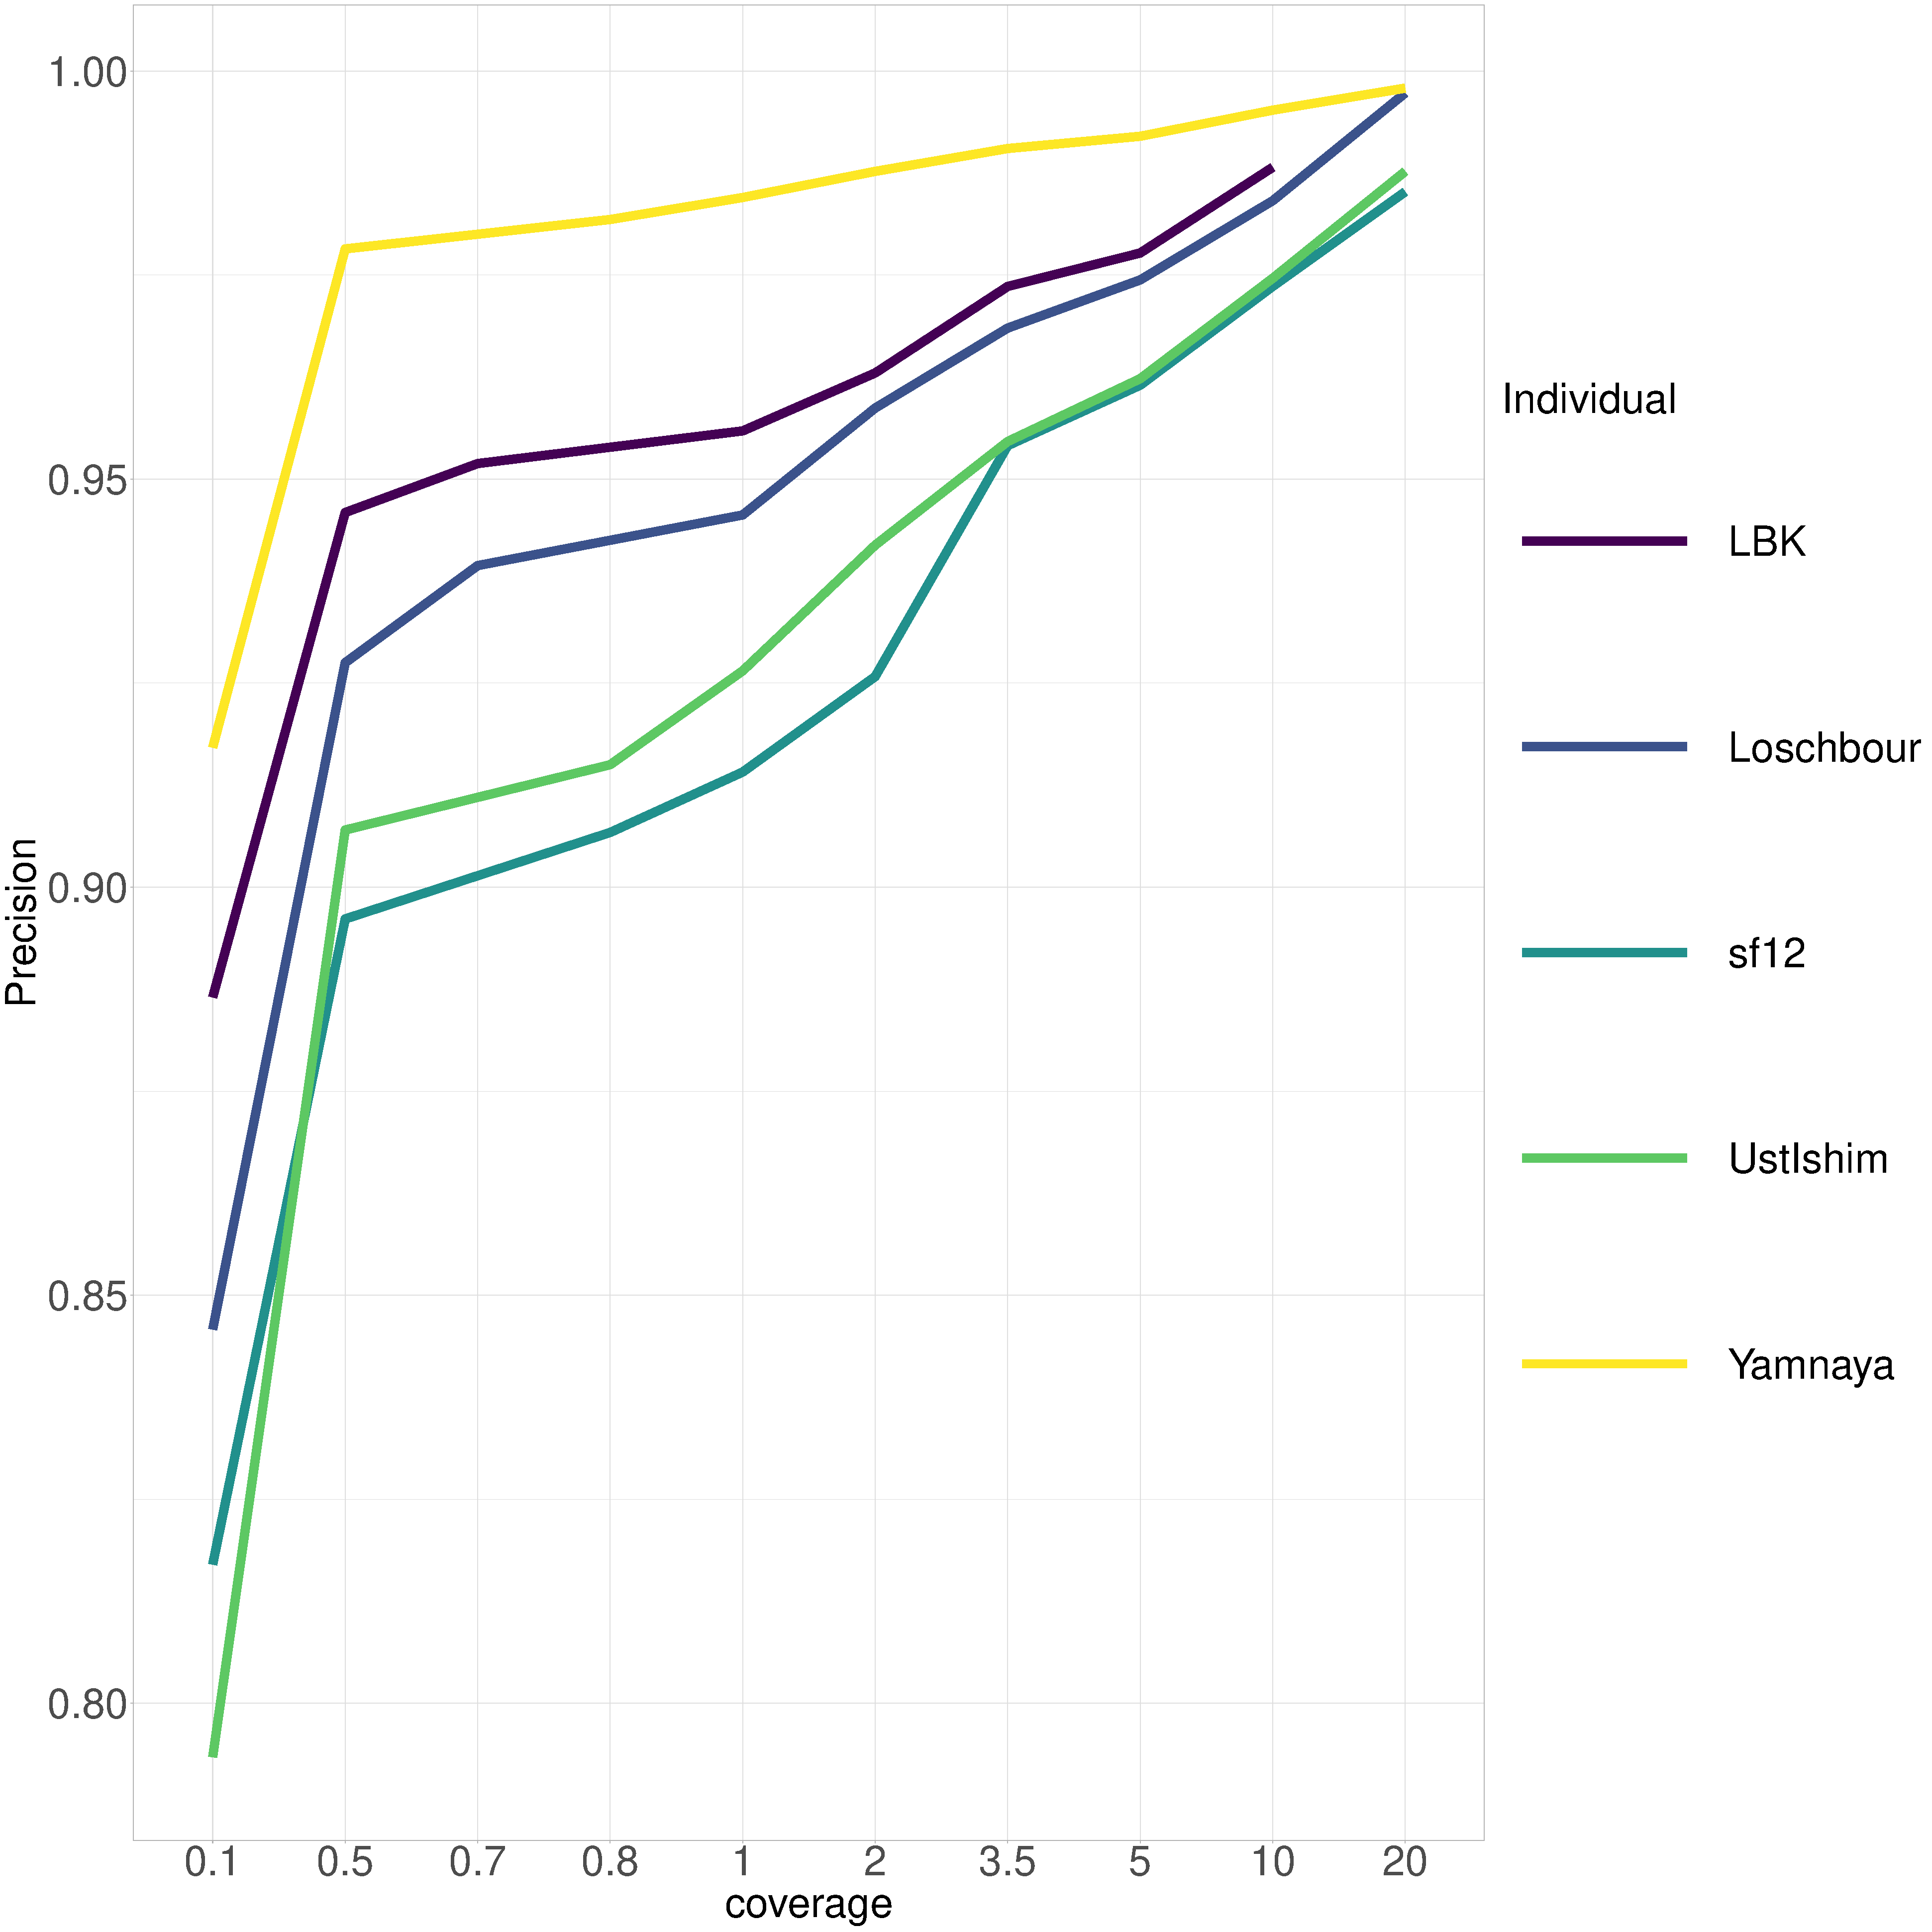
\includegraphics[width=1.0\textwidth]{../images/chapter1/allDownsampled_rtgtools_Precision.pdf}
    \caption{Precision of genotype calling at different coverages for different ancient individuals, assuming calls in the full coverage genome are correct,  calculated using rtg-tools.}
    \label{fig:precision_downsampled_rtgtools}
\end{figure}

As expected, both the overall sensitivity and precision of imputation fell with coverage, with a particularly sharp drop-off in both metrics between 0.5x and 0.1x coverage. Whilst I did not investigate this, other studies have shown the probability of any one SNP in an sample being correctly imputed depends strongly on the frequency in the reference panel \cite{hui2020evaluating, rubinacci2021efficient}. In particular, alleles which are rare in the reference panel are less likely to be imputed correctly.

Different downsampled individuals varied in the precision and sensitivity of genotype imputation. At all coverages, Yamnaya had the both the highest sensitivity and precision. This may be because the imputation reference panel contains a high proportion of present-day Europeans, who have a relatively higher porportion of recent Yamnaya-like ancestry relative to e.g. Hunter Gatherer-like ancestry \cite{Haak2005}. Many studies in present-day individuals have shown that imputation accuracy increases when more haplotypes which are close to the target individual are found in the reference panel \cite{HUANG2009235, delaneau2018integrative}. On the other hand, the sample Ust'Ishim is known to have contributed very little genetic ancestry to present-day populations \cite{Prufer2014} and may therefore have fewer closely matching haplotypes in the reference panel, and a correspondingly lower imputation accuracy. 

Imputation accuracy may also be related to demographic history. Populations which are known to have smaller effective population size, such as Western-Hunter Gathers, also contain longer tracts between individuals which are identical by descent (IBD) \cite{browning2015accurate} and fewer heterozygous positions. As imputation relies on matching IBD tracts between individuals, imputation accuracy increases where individuals share more IBD \cite{kong2008detection}. However, this would not be the case in this analysis as there are not hunter-gatherers in the reference panel for target hunter-gatherers to share IBD with. Additionally, switch-errors during the pre-phasing step of imputation may harm imputation accuracy, so a reduced density of heterozygous positions may result in increased accuracy. 

\subsection{Phasing accuracy}

I also used rtg-tools to calculate the number of phased heterozygous genotypes where the downsampled individual has the same phasing as the full coverage individual (Fig \ref{fig:phasing_performance_downsampled}). I note that this should not be considered to be the same as estimating the switch error rate, since we do not know that the phasing in the full-coverage individual is the true phase. However, this can be used as a rough proxy for switch errors, since it is known that phasing in lower coverage individuals is likely to be less accurate than those in the high coverage individuals \cite{rubinacci2021efficient}.

\begin{figure}[htp]
    \centering
    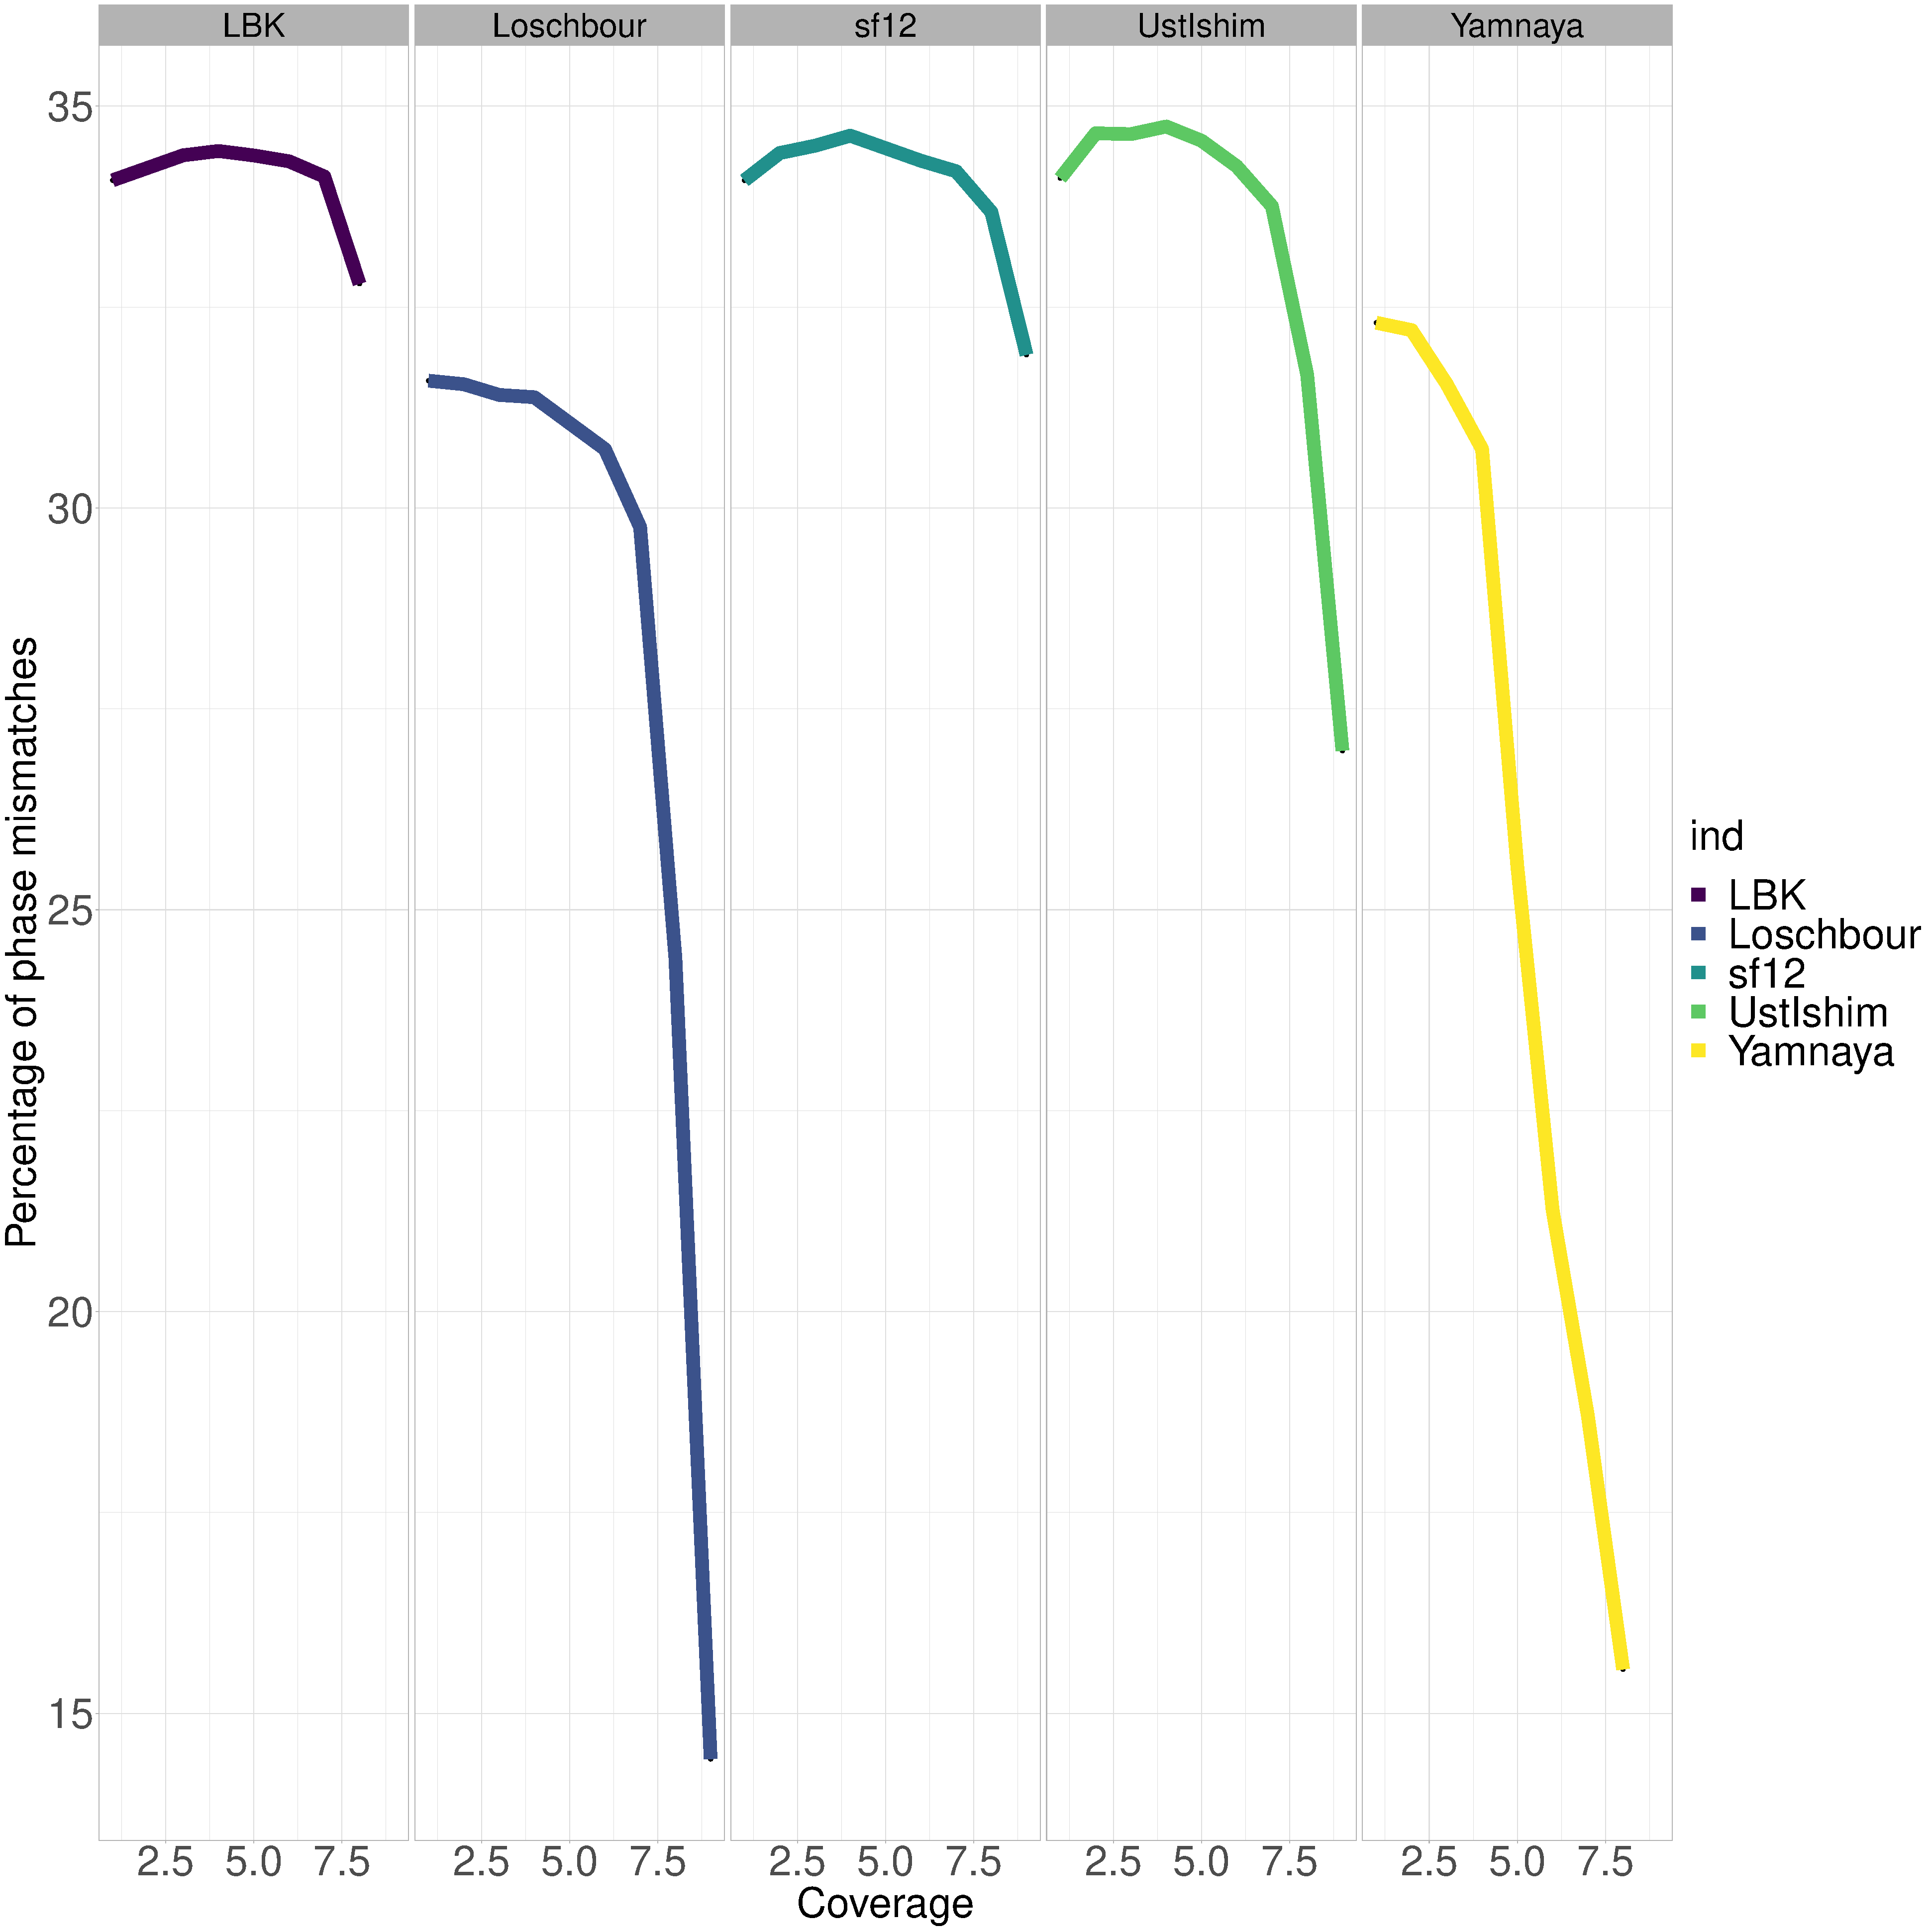
\includegraphics[width=1.0\textwidth]{../images/chapter1/phasing_performance_downsampled.pdf}
    \caption{Percentage of phased genotypes which agree with the same full-coverage sample for each individual and each level of downsampling. Genotypes with phase deemed unresolvable by rtg-tools were excluded from the calculations. Note that these numbers are given as incorrect / (incorrect + correct - unresolved) and so values are in part driven by the relative heterozygosity of each sample.}
    \label{fig:phasing_performance_downsampled}
\end{figure}

\subsection{Validating posterior probability calibration}

GLIMPSE estimates genotype probabilities at each SNP within each individual, giving the posterior probability that a given genotype within a single individual is correctly called. I assessed how well-calibrated these probabilities are in the Yamnaya 0.1x downsampled individual, using the maximum genotype likelihood at each of the approximately 77 million positions which were processed by GLIMPSE. A high $max(GL)$ for a particular genotype (i.e.\ 0.99) corresponds to a high confidence in the genotype. Alternatively a flat $max(GL)$ (i.e.\ 0.33) corresponds to no information about the genotype. 

I split the genome into 10,000 equally-sized bins according to $max(GL)$. For each bin, I calculated both the proportion of SNPs which were correctly imputed (i.e.\ that matched the same high coverage individual) and the mean $max(GL)$ (Fig. \ref{fig:Yamnaya_0.1x_GL_calibration}). If the genotype probabilities are well calibrated, we would expect to see a clear positive linear relationship between $max(GL)$ probability and the probability that genotype matches the full-coverage sample.

\begin{figure}[htp]
    \centering
    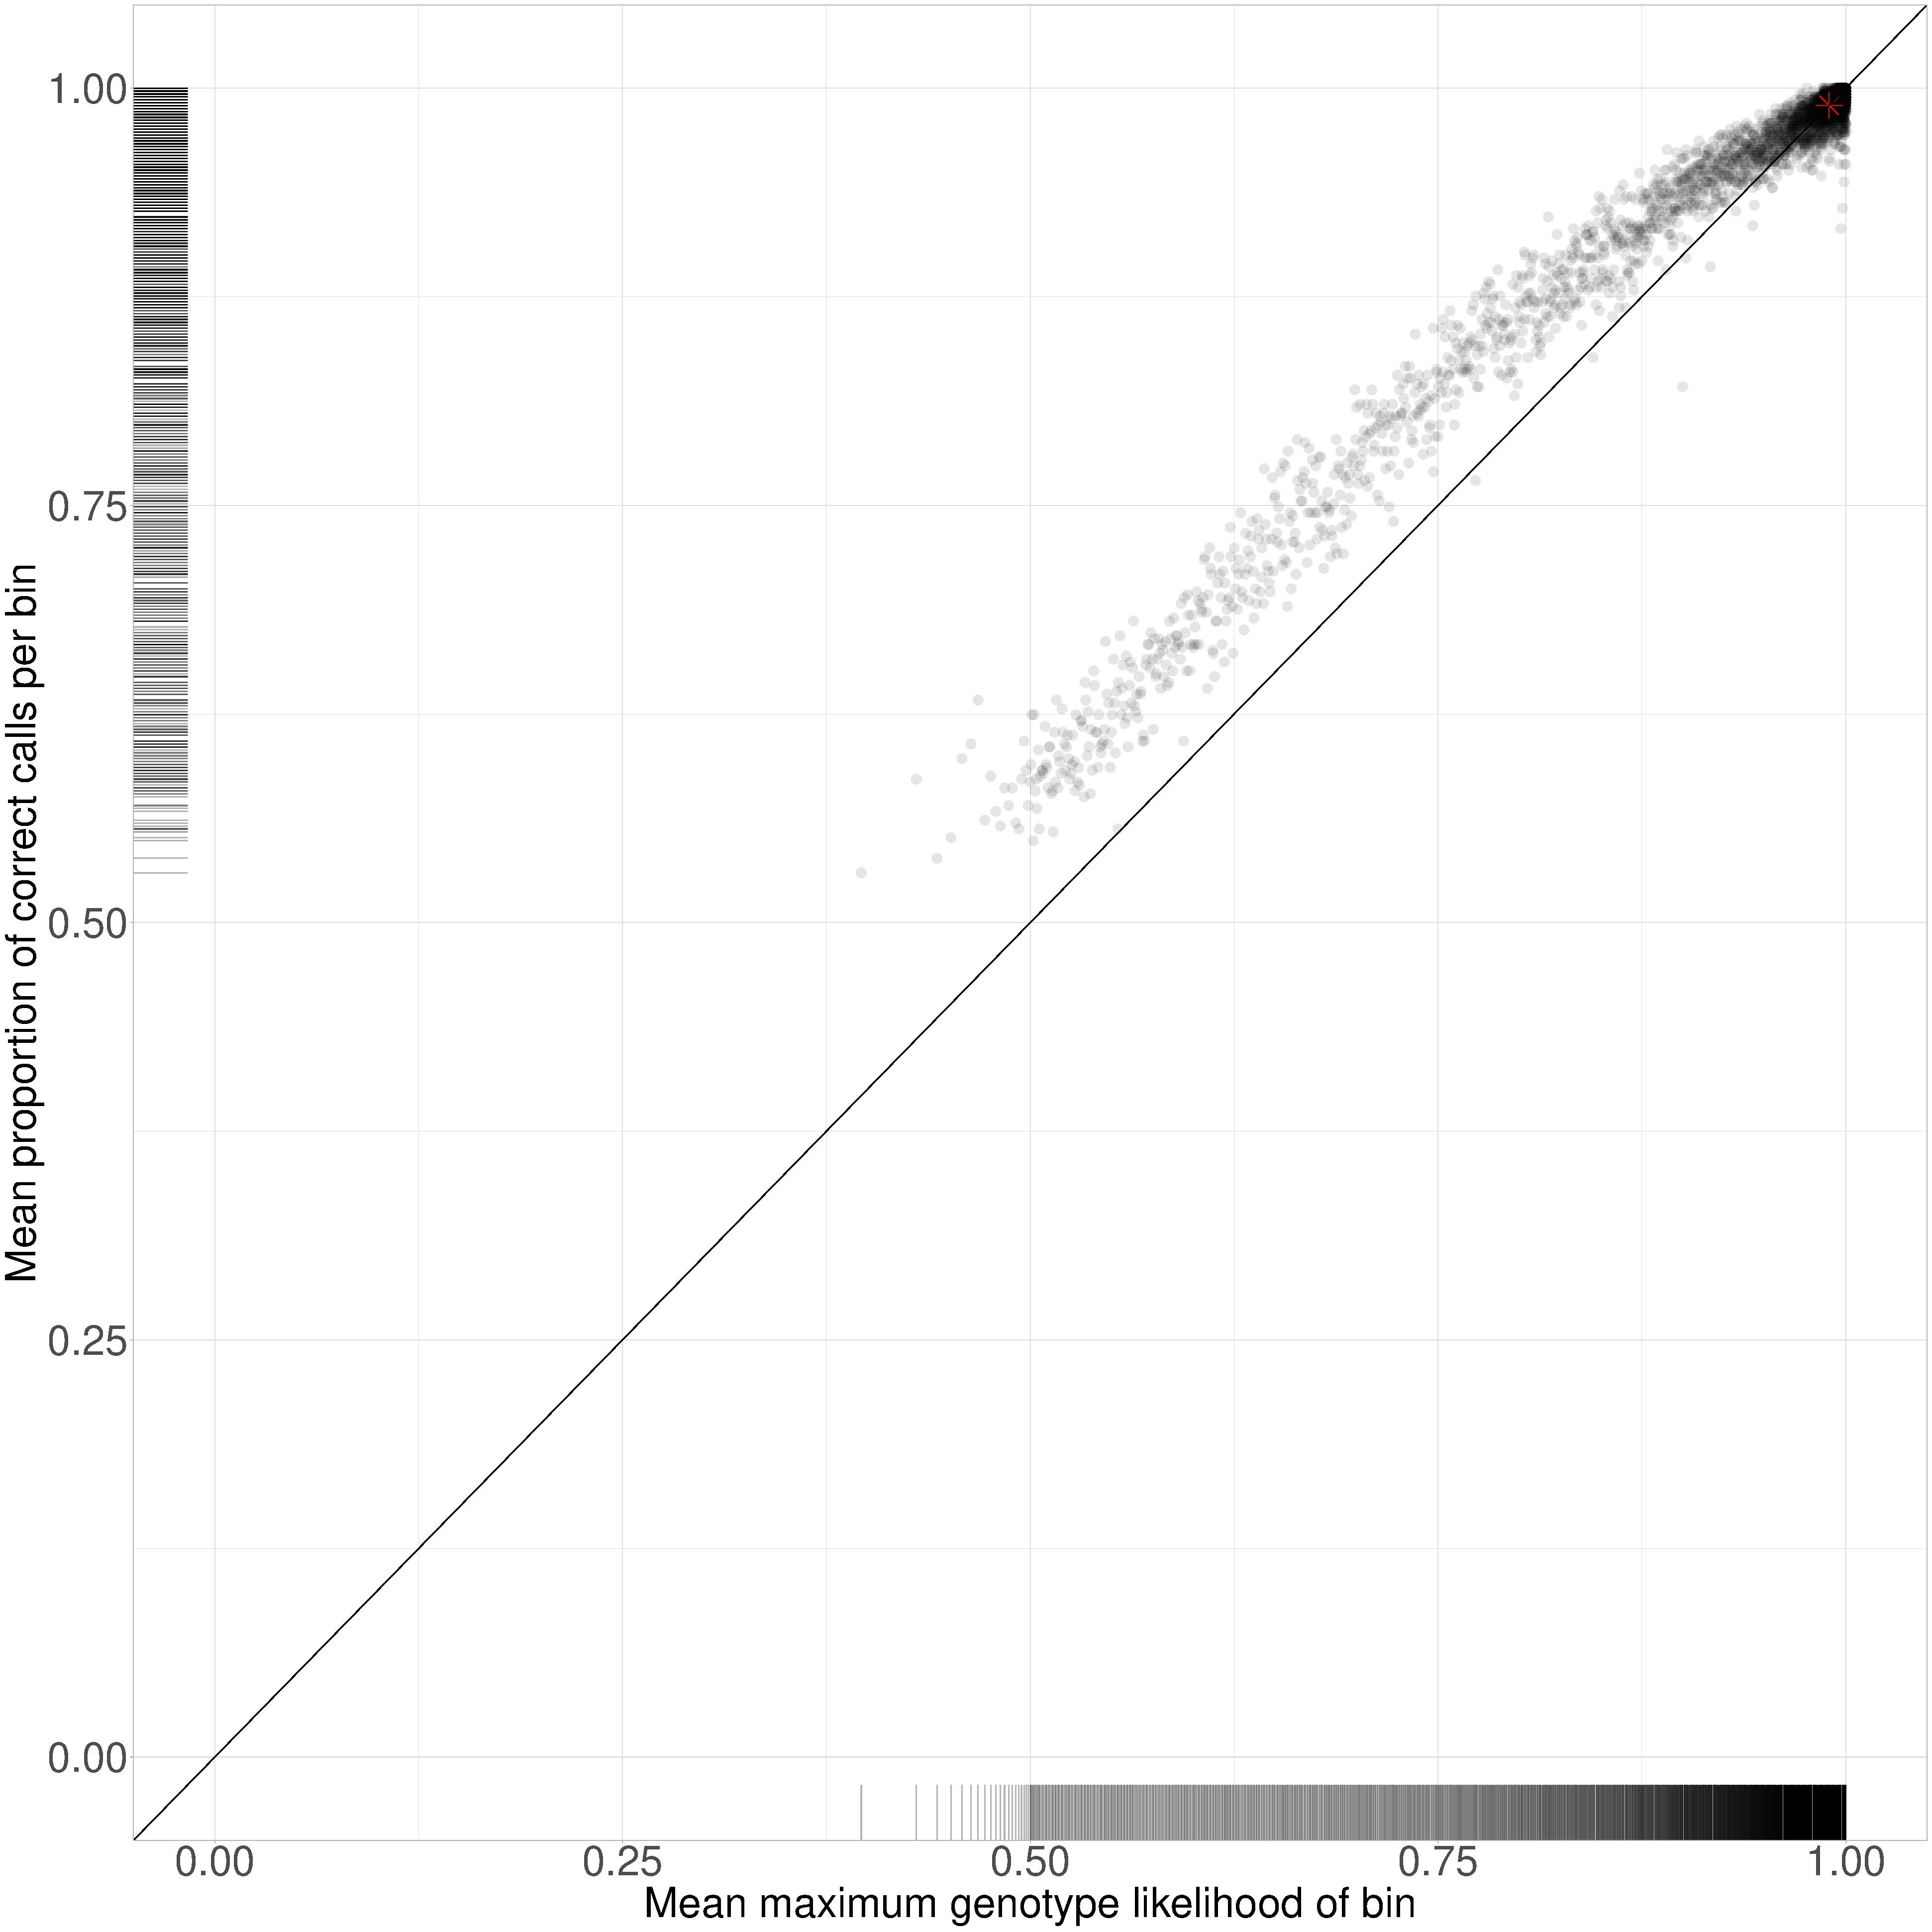
\includegraphics[width=1.0\textwidth]{../images/chapter1/Yamnaya_0.1x_bin.pdf}
    \caption{Relationship between genotype likelihood and probability of genotype call being correct for Yamnaya downsampled to 0.1x coverage. Genome binned by maximum posterior genotype likelihood and mean maximum posterior genotype likelihood (x-axis) and proportion of correct calls calculated per bin (y-axis). Rugs on each margin show the distribution of x and y values. Black line is $y=x$.}
    \label{fig:Yamnaya_0.1x_GL_calibration}
\end{figure}

The probabilities are well calibrated (r-squared = 0.981) and could therefore be useful for downstream analysis. It should be noted that they are slightly conservative, in that a majority of the points in Fig. \ref{fig:Yamnaya_0.1x_GL_calibration} are above the line of equality. For example, the mean proportion of correct genotypes within all bins where $0.73 < max(GL) < 0.76$ was 82\%. I performed the same analysis using different samples at different levels of coverage and the results were qualitatively similar (Supplementary Figure. \ref{fig:UstIshim_0.1x_bin}).

\subsection{ChromoPainter analysis} \label{sec:ChromoPainterChap2}

To assess the impact of coverage on ChromoPainter analysis, I merged the dataset of downsampled individuals with the `standard set' of ancient reference individuals (124 ancient samples $>2$X coverage) and performed an `all-v-all' painting of the merged dataset, which separately paints each individual as a recipient using all other individuals in the dataset as donors. The `all-v-all' painting was necessary to paint the 124 `standard set' of individuals against one another so that they can act as surrogates in later SOURCEFIND analysis. 

I was interested to see whether a downsampled individual and full coverage had similar copyvectors, or in other words, whether they matched similar amounts to the same donor individuals. To do this, I estimated $TVD$ between the copyvectors of the full coverage and downsampled individuals. $TVD$ is a distance metric which gives a measure of dissimilarity between two copyvectors.

Fig. \ref{fig:CP_correlation_allSamples_0.1x_0.5x_30x} displays the relationship between copyvectors for each downsampled individual and the corresponding full coverage individual for both 0.1x and 0.5x coverage. Each individuals' copyvectors were estimated using the same set of ancient samples as donors.

\begin{figure}[htp]
    \centering
    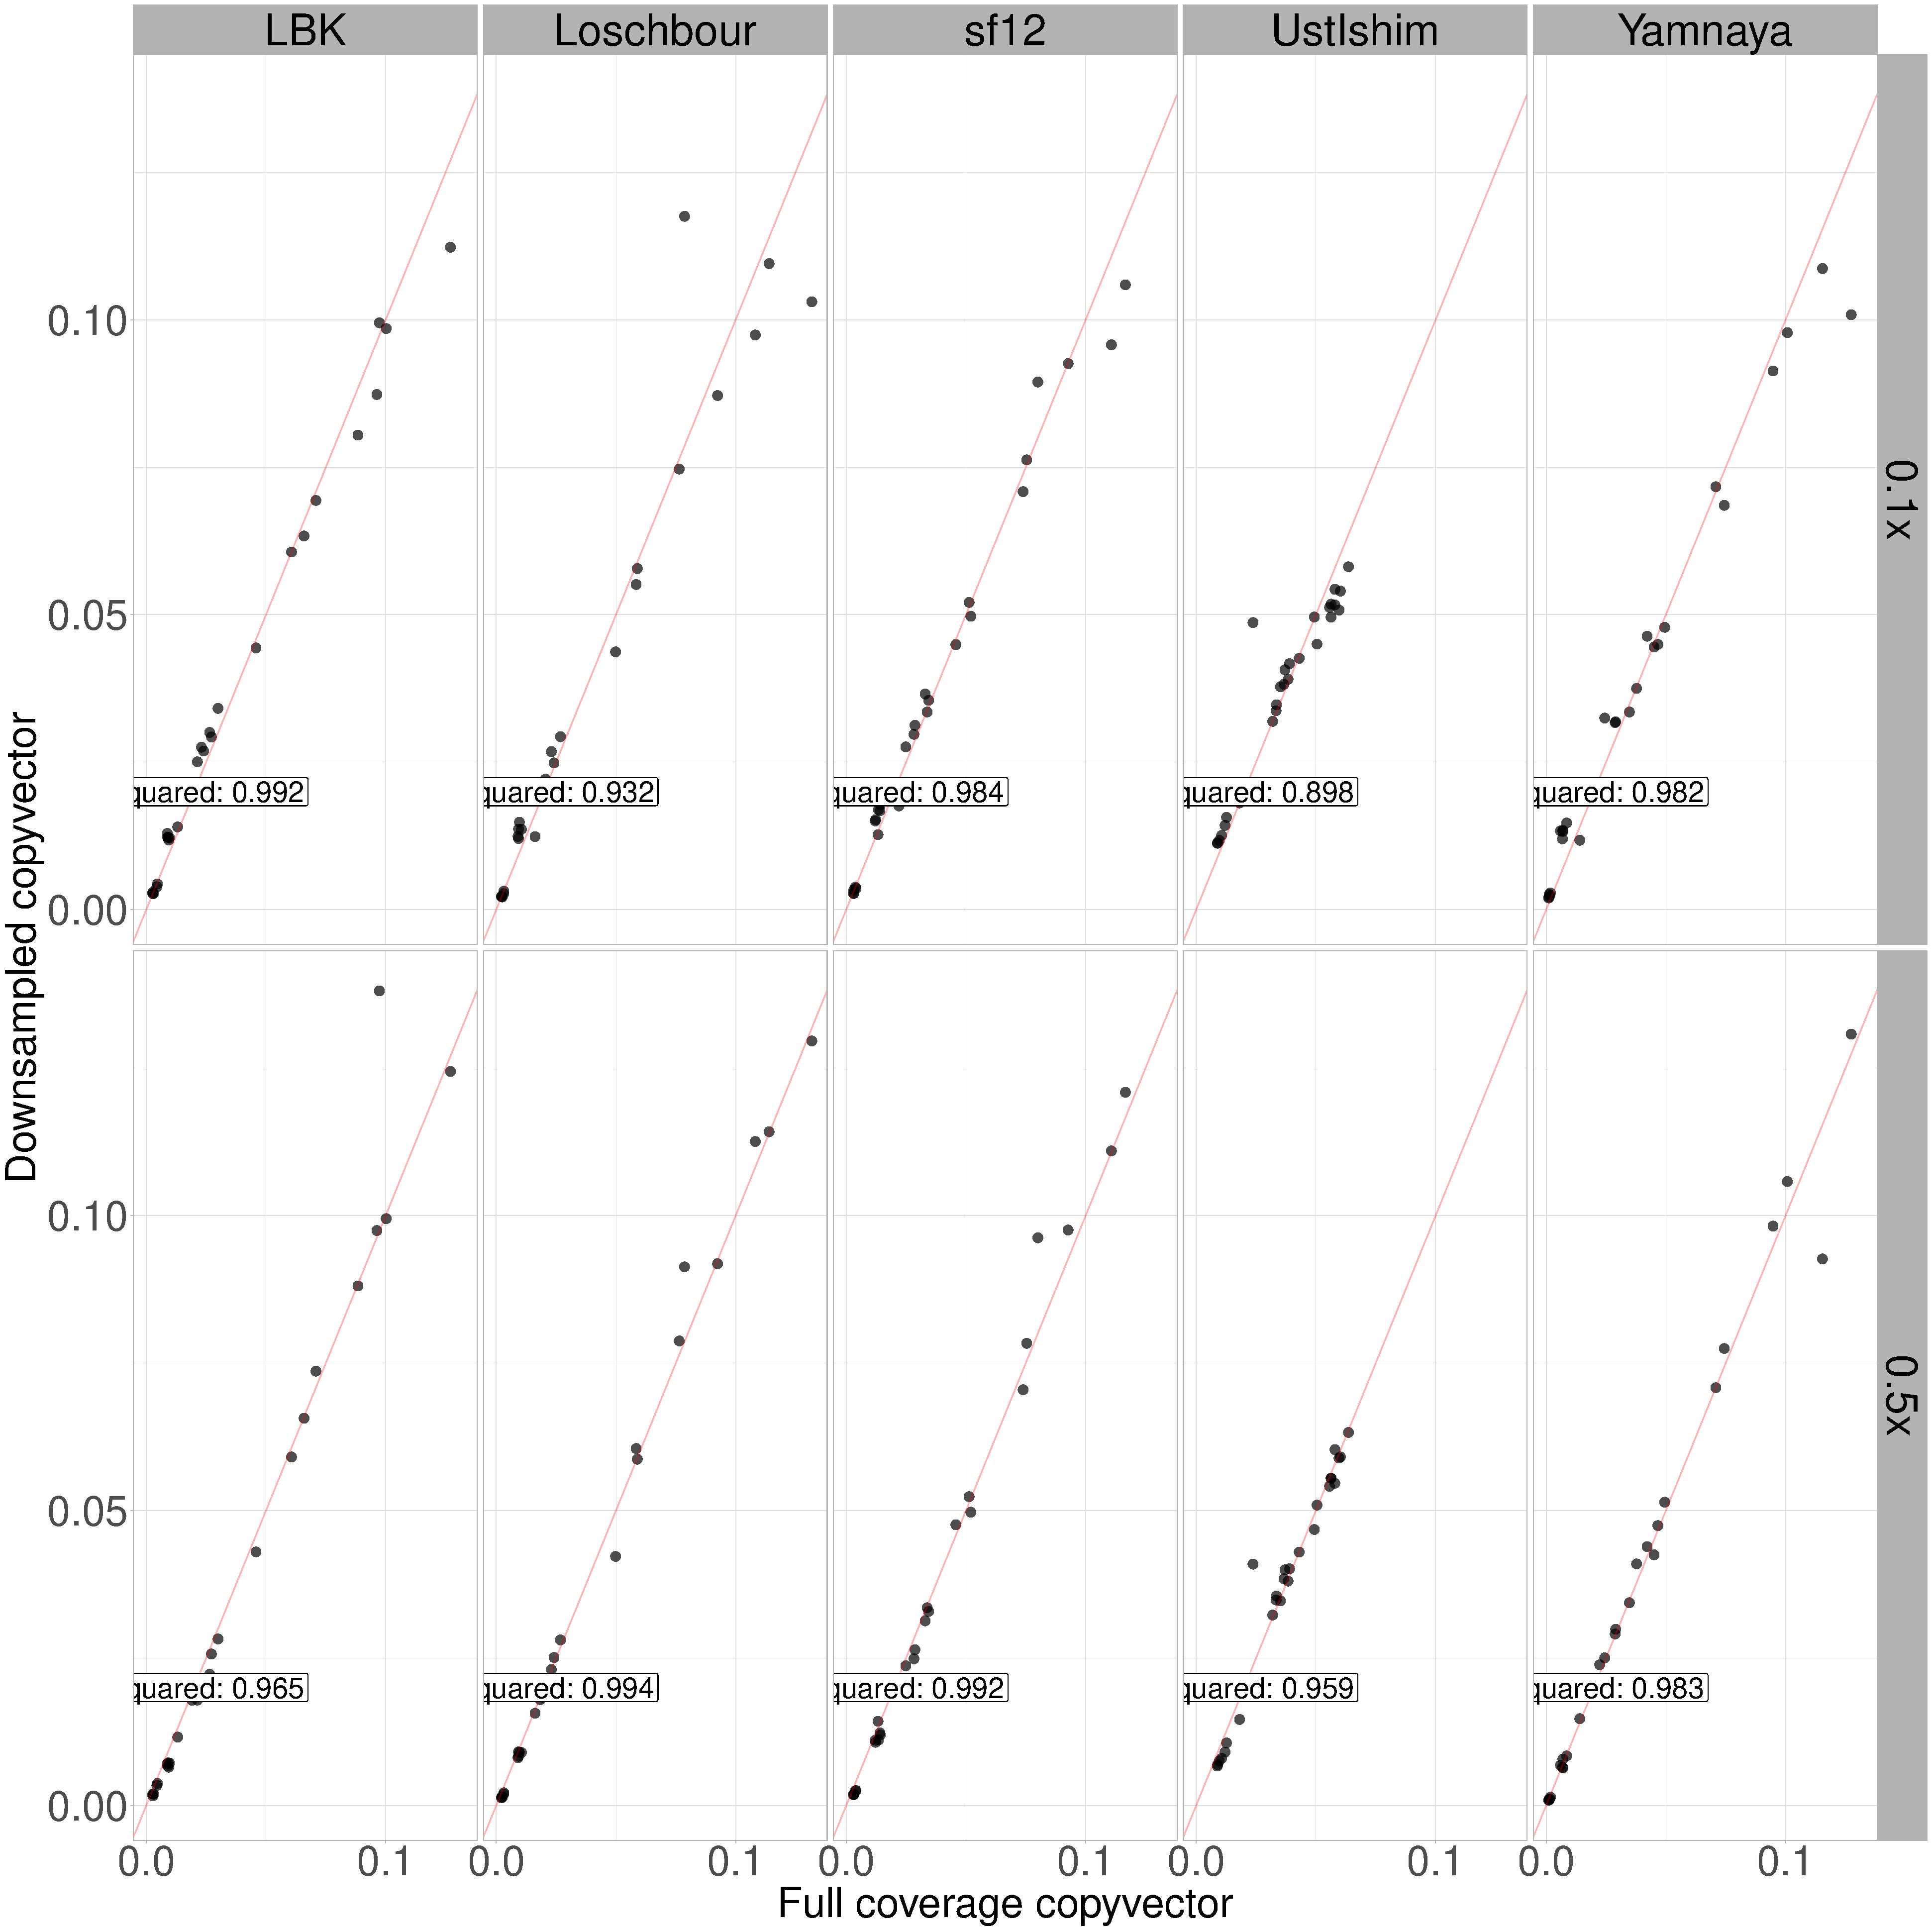
\includegraphics[width=1.0\textwidth]{../images/chapter1/CP_correlation_allSamples_0.1x_0.5x_30x.pdf}
    \caption{For five different samples (columns), the proportion of DNA that each downsampled (y-axis) or full coverage (x-axis) genome matches to each of 125 ancient individuals (dots). Results are shown for 0.1x (top row) and 0.5x (bottom row) downsampled genomes. Points coloured by manual assignment to broad-scale populations. Red line is line of equality ($y=x$). x and y units are normalised copying values and thus removed for clarity.}
    \label{fig:CP_correlation_allSamples_0.1x_0.5x_30x}
\end{figure}

As expected, the TVD between the full-coverage and downsampled copyvectors decreased with coverage. The 0.1x genome had a substantially increased TVD, similar to the much reduced imputation accuracy. For each of the genomes downsampled to 0.1x, a particular difference to the 0.5x downsampled genomes is that the lowest contributing donors contribute more to the 0.1x downsampled genome than to the full coverage genome and that the highest contributing donors contribute less to the 0.1x genome than they do the full coverage genome. Put in other words, the copyvectors at 0.1x are tending towards becoming more `flat', or copying the same amount from each donor individual. 

This can also be seen as `regressing to the prior'. In this case, the prior is copying an equal amount to each donor individual. This can be visualised explicitly by calculating TVD between each downsampled genome and a flat prior, a vector of length $D$, where $D$ is the total number of donor individuals and each element of $D$ is equal to 1 / $D$ (Fig. \ref{fig:TVD_ancients_flat_prior}). This clearly shows the reduced TVD to the flat copyvector for the 0.1x individual relative to other coverages. In later sections, I will discuss whether this is `noise' or `bias' induced by imputation, i.e.  whether copying is regressing to the prior in a similar manner for all samples. 

\begin{figure}[htp]
    \centering
    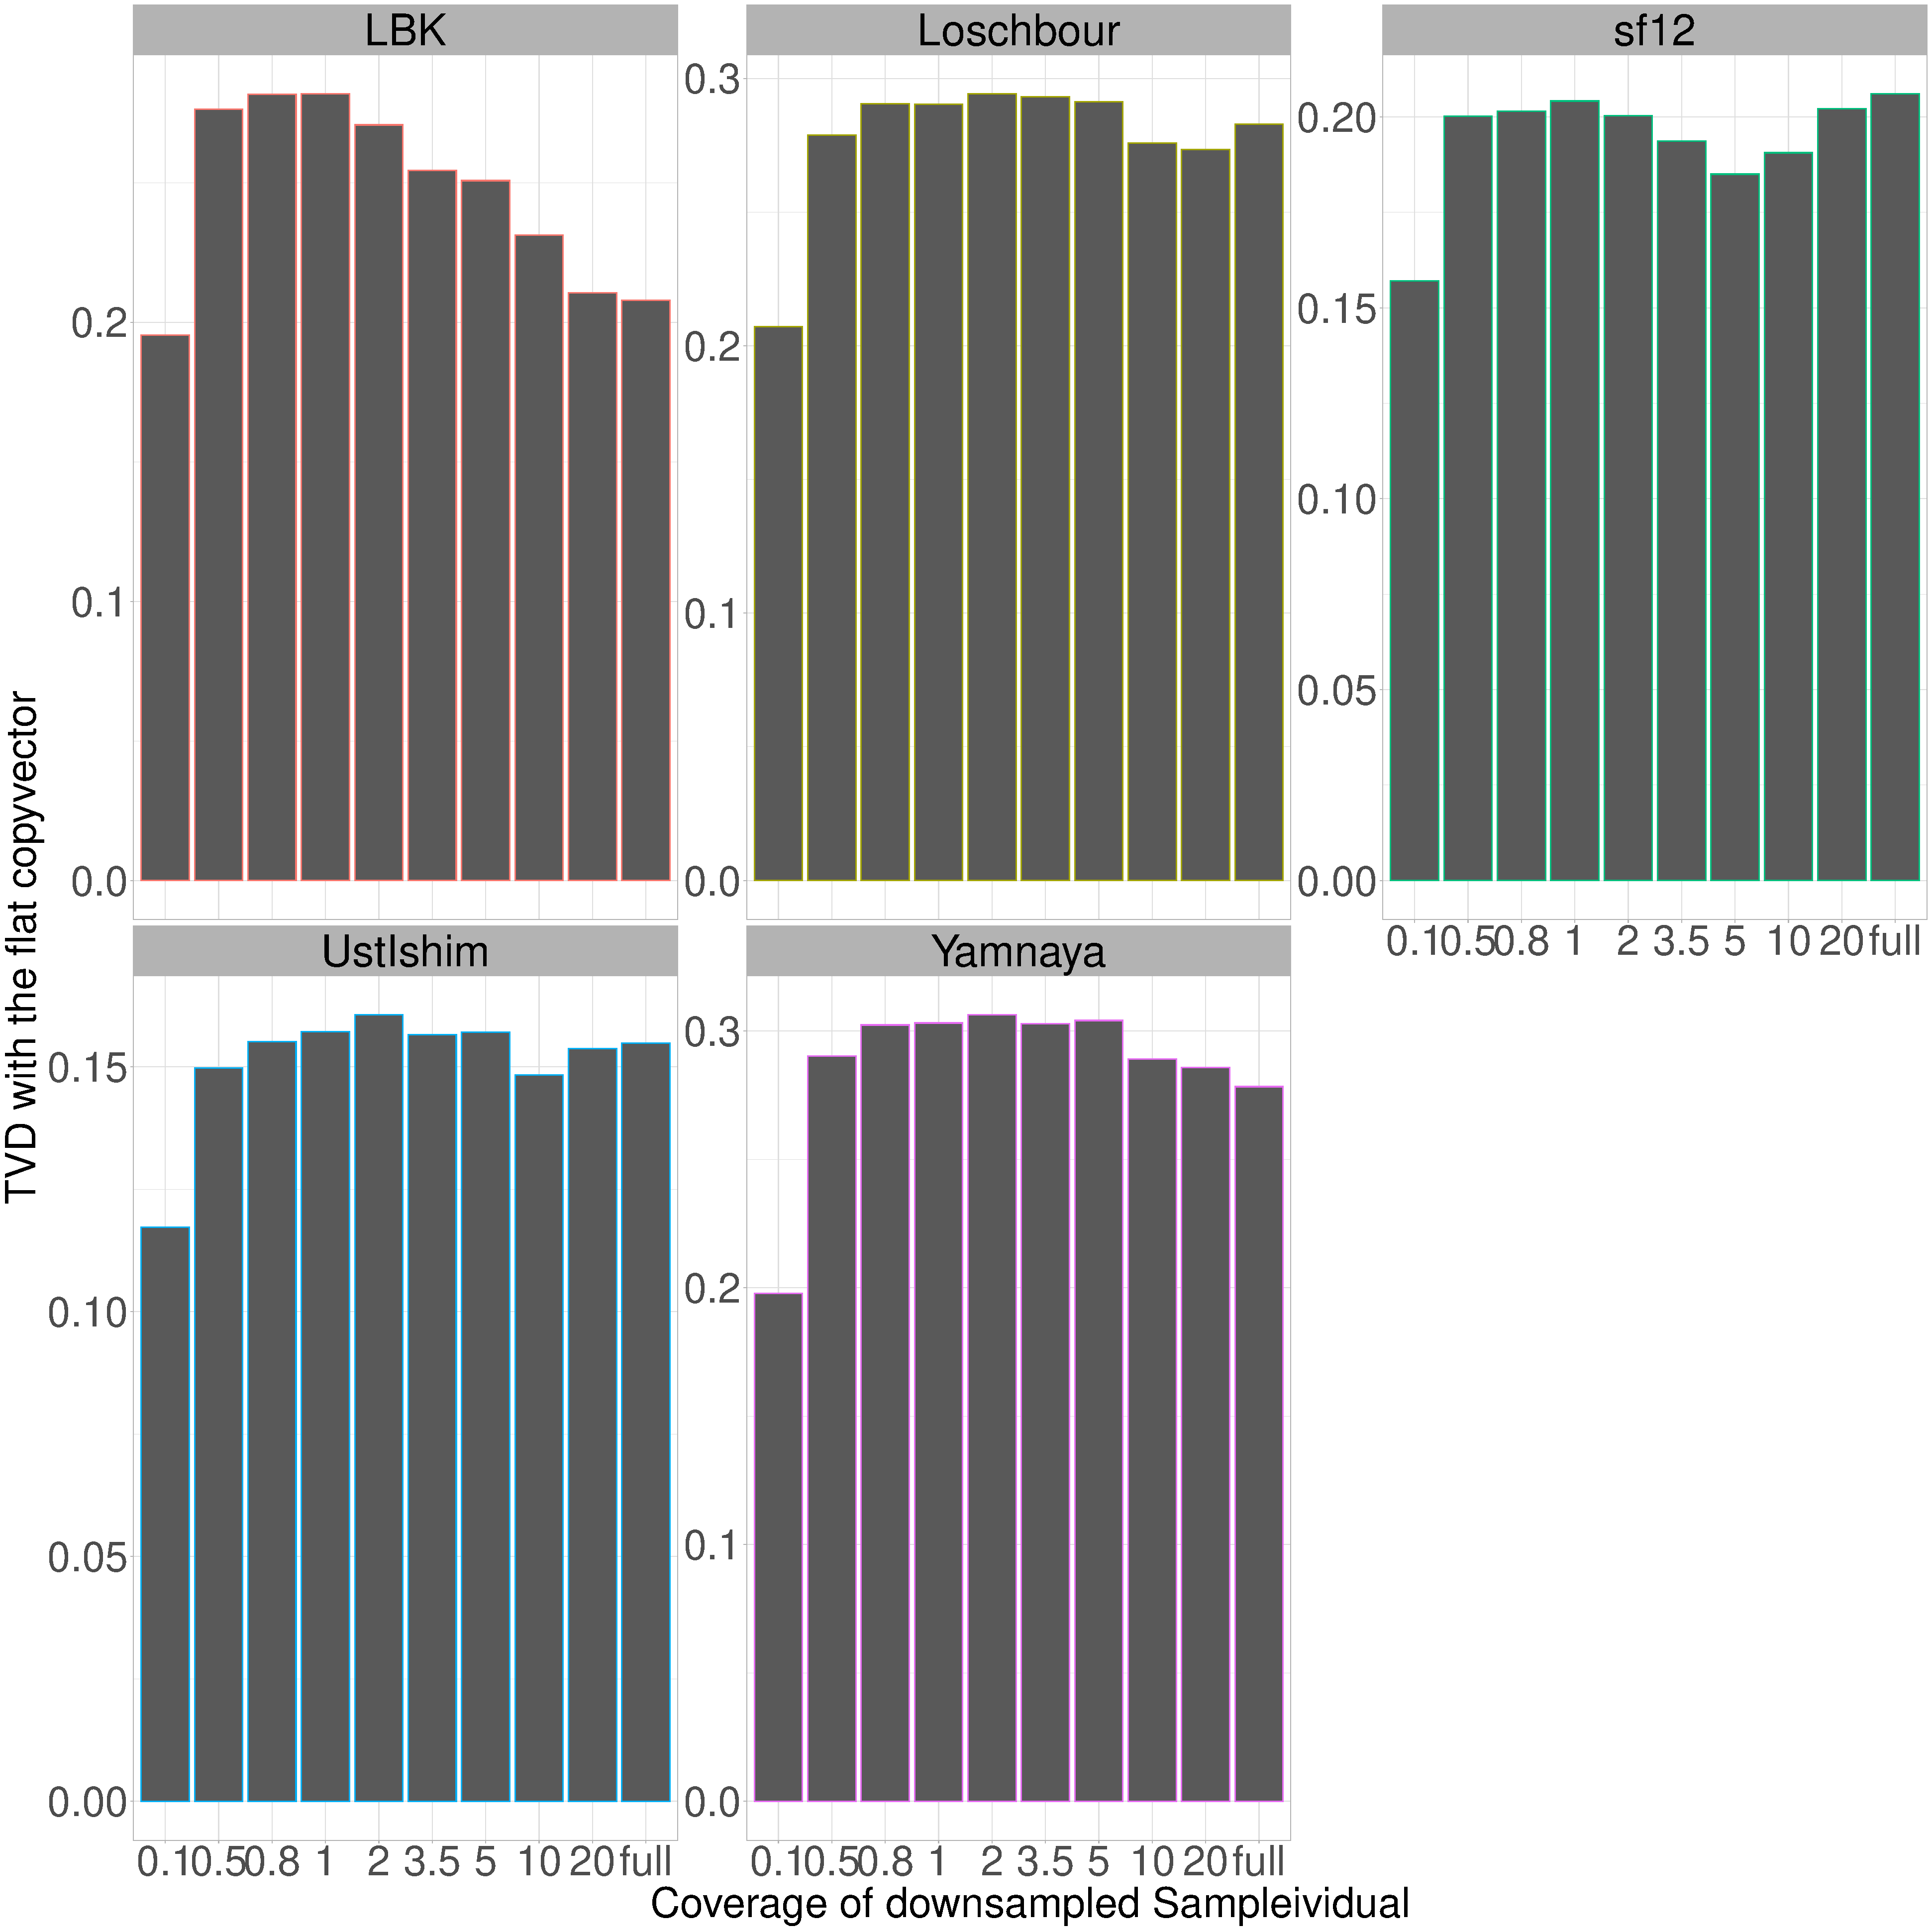
\includegraphics[width=1.0\textwidth]{../images/chapter1/TVD_ancients_flat_prior.pdf}
    \caption{TVD (metric of copyvector dissimilarity between two individuals) between each downsampled ancient individual and a flat copyvector. Flat copyvector equivalent to a vector of length $N$ where each element = $1/N$.}
    \label{fig:TVD_ancients_flat_prior}
\end{figure}

I also considered the effect of coverage on the copyvectors estimated when using present-day individuals from the 1000 genomes project as donors (Fig. \ref{fig:CP_correlation_allSamples_0.1x_0.5x_30x_moderns}). Painting ancient samples using present-day donors is often useful, particularly with more recent ancient samples, as there may not be enough relevant ancient samples to paint the ancients with. I merged the downsampled and full coverage ancient individuals with the thousand genomes dataset (described in detail in Appendix section \ref{section:1000genomes}). As was the case with the all-v-all ancients painting, the TVD between copyvectors was highest for the 0.1x individuals. However, the copyvectors show a strong correlation / low TVD for 0.5x individuals. 

It should be noted that utility of painting different ancient individuals with a modern reference panel depends on the ancestry and age of the ancient sample. The spread of points along the $y=x$ line in Fig. \ref{fig:CP_correlation_allSamples_0.1x_0.5x_30x_moderns} shows how much a particular ancient recipient preferentially copies more from particular modern population over others. LBK, for example, has points which are spread evenly across $y=x$, showing that they copy much more from some populations than others, suggesting modern populations are good for distinguishing this particular ancient sample. On the other hand, the points for Ust'Ishim are shrunk towards lower values of $y=x$, showing that the copyvector is relatively flat and that it does not preferentially copy from some populations to the same degree that LBK does. This is consistent with findings that UstIshim did not contribute ancestry towards present-day populations \cite{Fu2014}. Accordingly, relatively less useful information is obtained from painting Ust'Ishim with a modern reference panel than LBK.

\begin{figure}[htp]
    \centering
    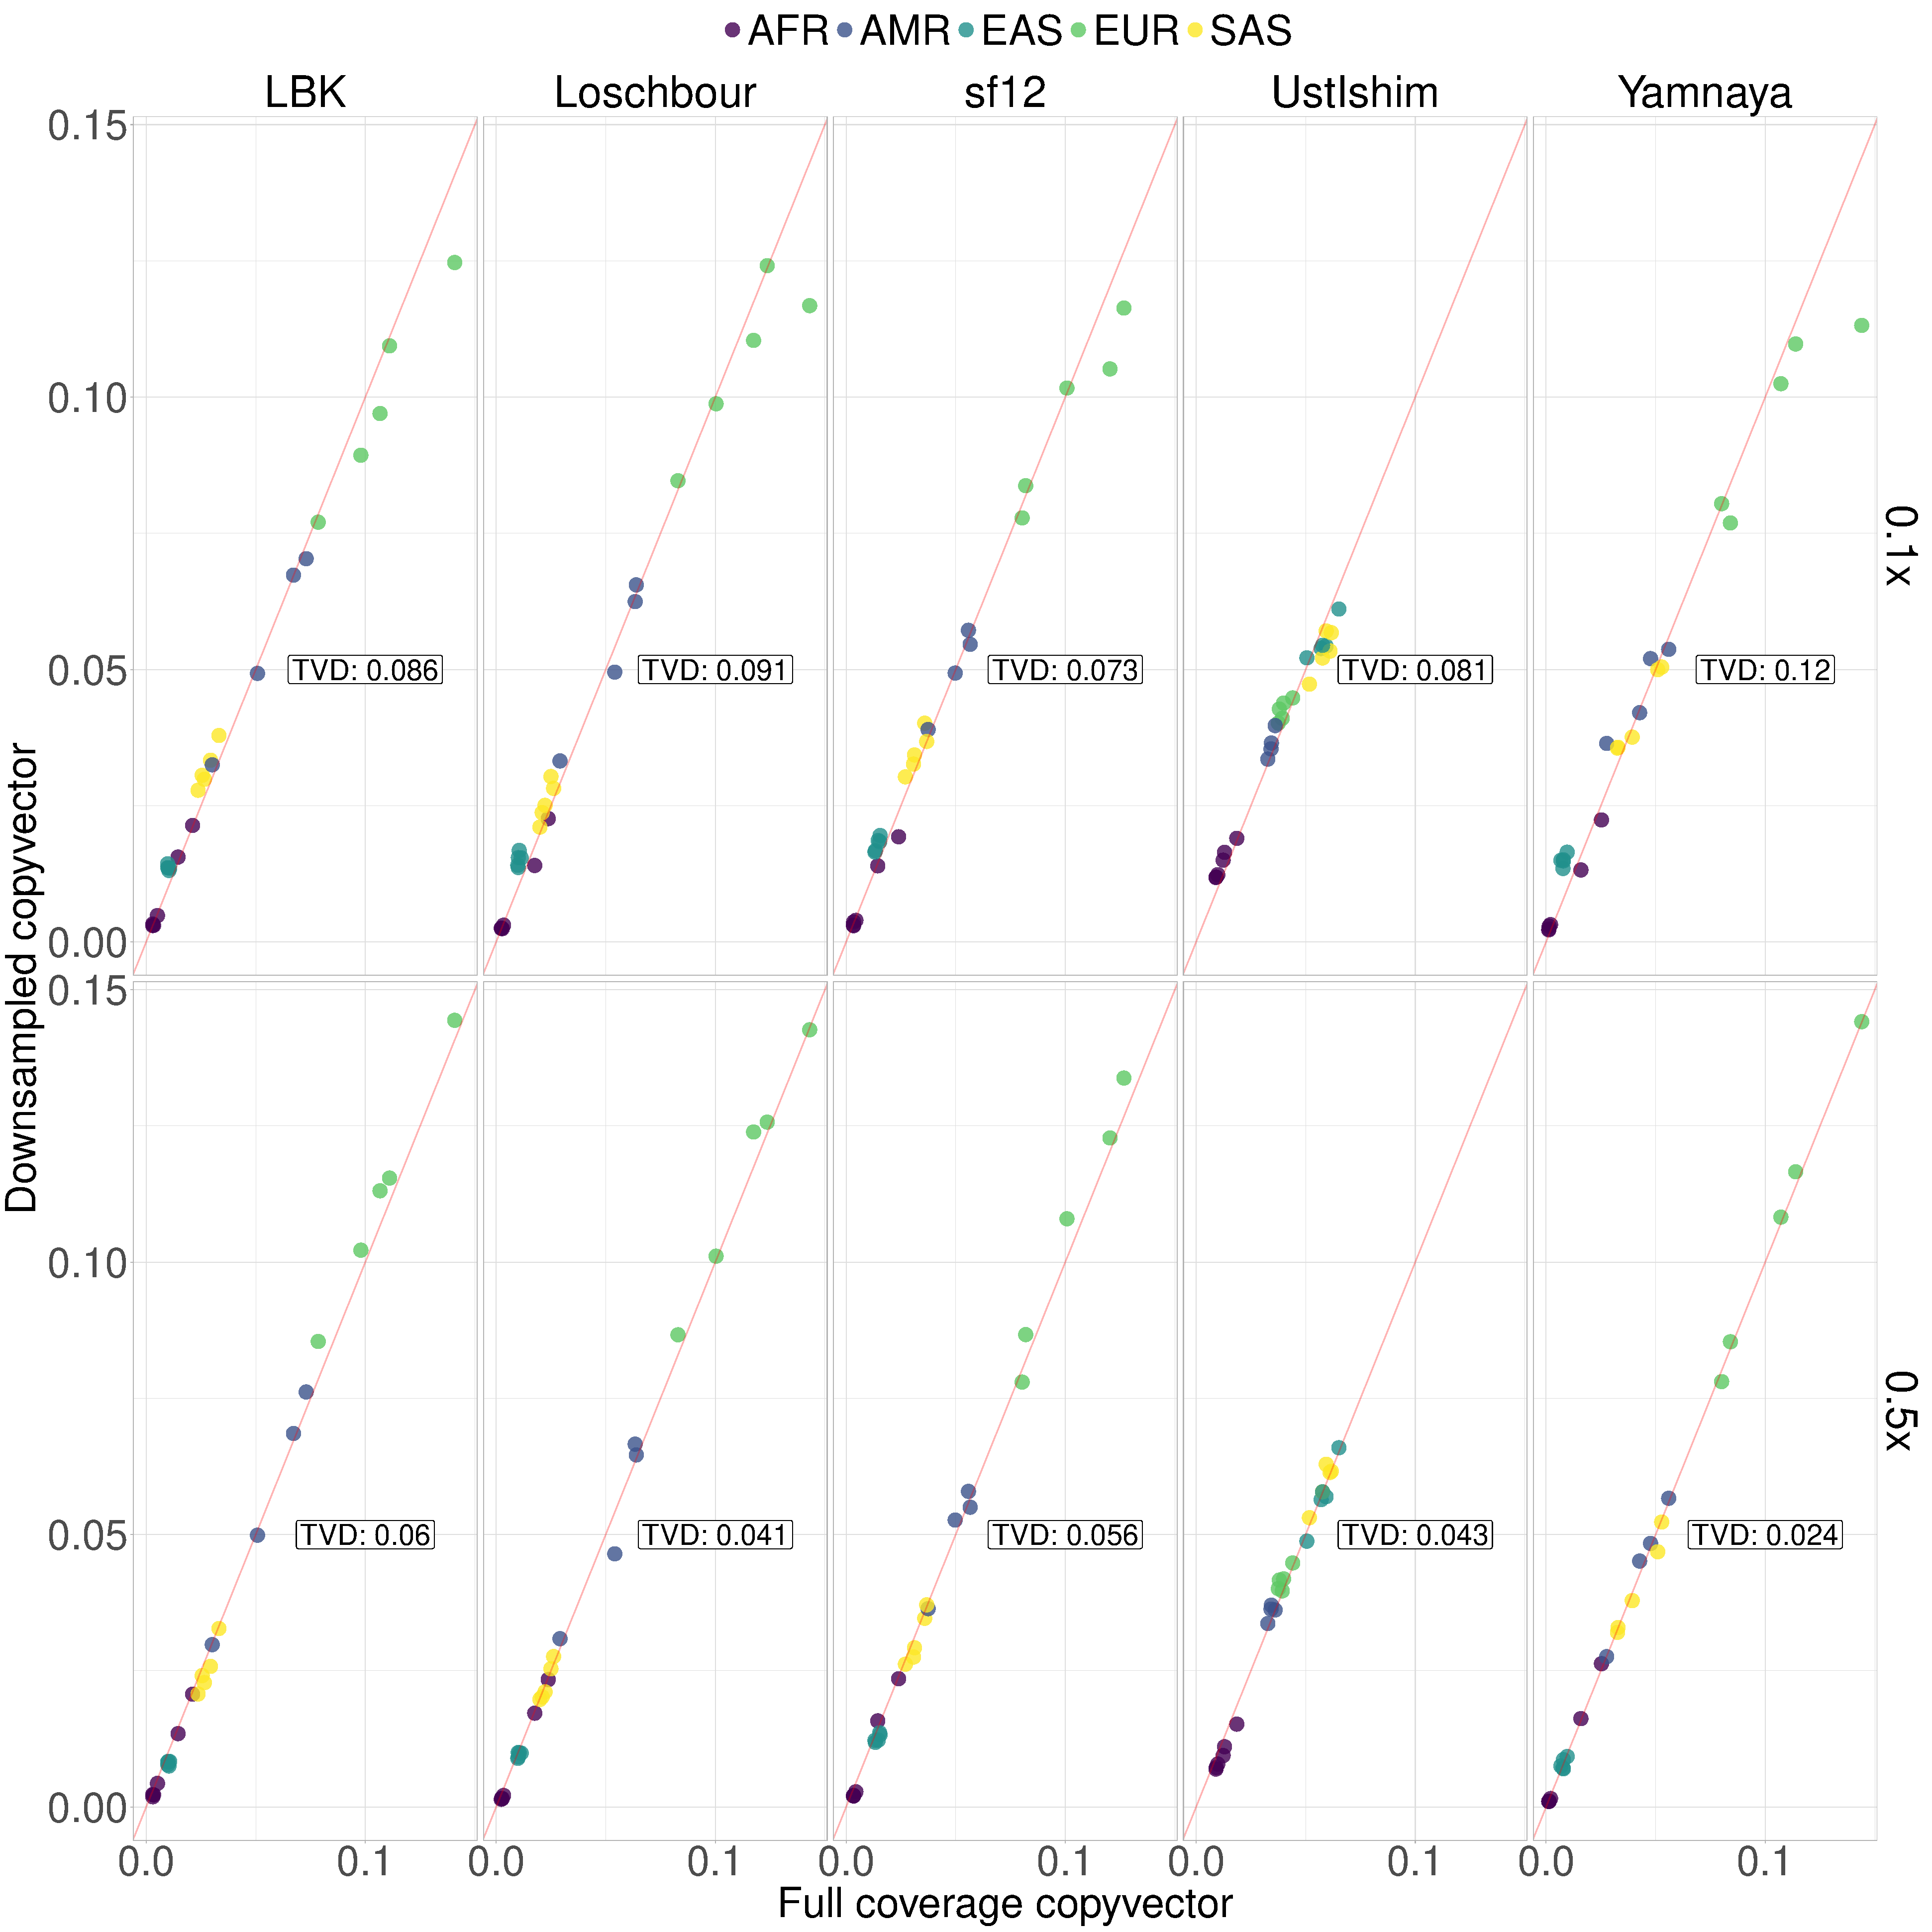
\includegraphics[width=1.0\textwidth]{../images/chapter1/CP_correlation_allSamples_0.1x_0.5x_30x_moderns.pdf}
    \caption{For five different samples (columns), the proportion of DNA that each downsampled (y-axis) or full coverage (x-axis) genome matches to individuals from each of 26 present-day populations (dots). Red line is $y=x$. x and y units are normalised copying values and thus removed for clarity. Points coloured by meta-population.}
    \label{fig:CP_correlation_allSamples_0.1x_0.5x_30x_moderns}
\end{figure}

Principle component analysis (PCA) is a widely used technique to visualise the relative genetic diversity of different individuals. PCA can be performed on the chunklengths matrix in a similar way to how PCA on the genotype dosage matrix is often employed in ancient DNA studies. Visualising whether downsampled individuals cluster close to the same sample at full-coverage is a useful way of determining whether the copyvectors of the downsampled individual reflect those of the full-coverage individual.

The position of the full coverage individuals are consistent with prior knowledge about their ancestry (Fig. \ref{fig:PCA_panel_allInds_allCoverage}). For example, Loschbour is positioned alongside other Hunter Gatherers, who are highly differentiated from the later Neolithic farmers and Bronze Age Europeans. sf12 clusters with the other Scandinavian Hunter Gatherers in the dataset. Yamnaya is differentiated from the group of Bronze Age individuals and situated close to individuals from the Poltavka and Srubnaya culture. LBK is located with other individuals from the early to middle Neolithic in central Europe. Consistent with sharing little ancestry with any group over another, UstIshim is positioned close to the central Bronze Age mass, where most of the individuals in the PCA are located. 

For all levels of downsampling other than the 0.1x, the downsampled and full coverage genomes were positioned very closely to one another on the PCA. When considering all downsampled individuals, a pattern emerges whereby the genome downsampled to 0.1x for each individual is `pulled' towards the origin of the PCA. This may reflect a `homogenisation' of low coverage genomes when many genotypes are imputed.

To formally examine the positioning of the samples on the PCA, I calculated the closest Cartesian neighbour to each of the downsampled individuals, not including other downsampled individuals (Table \ref{tab:ClosestNeighbour}). Other than at 0.1x coverage, the samples UstIshim, sf12 and Loschbour always were closest to the same sample at full coverage. Up to 5x coverage, Yamnaya was closest to closely related YamnayaSamara and Poltavka samples. 


\begin{figure}[htp]
    \centering
    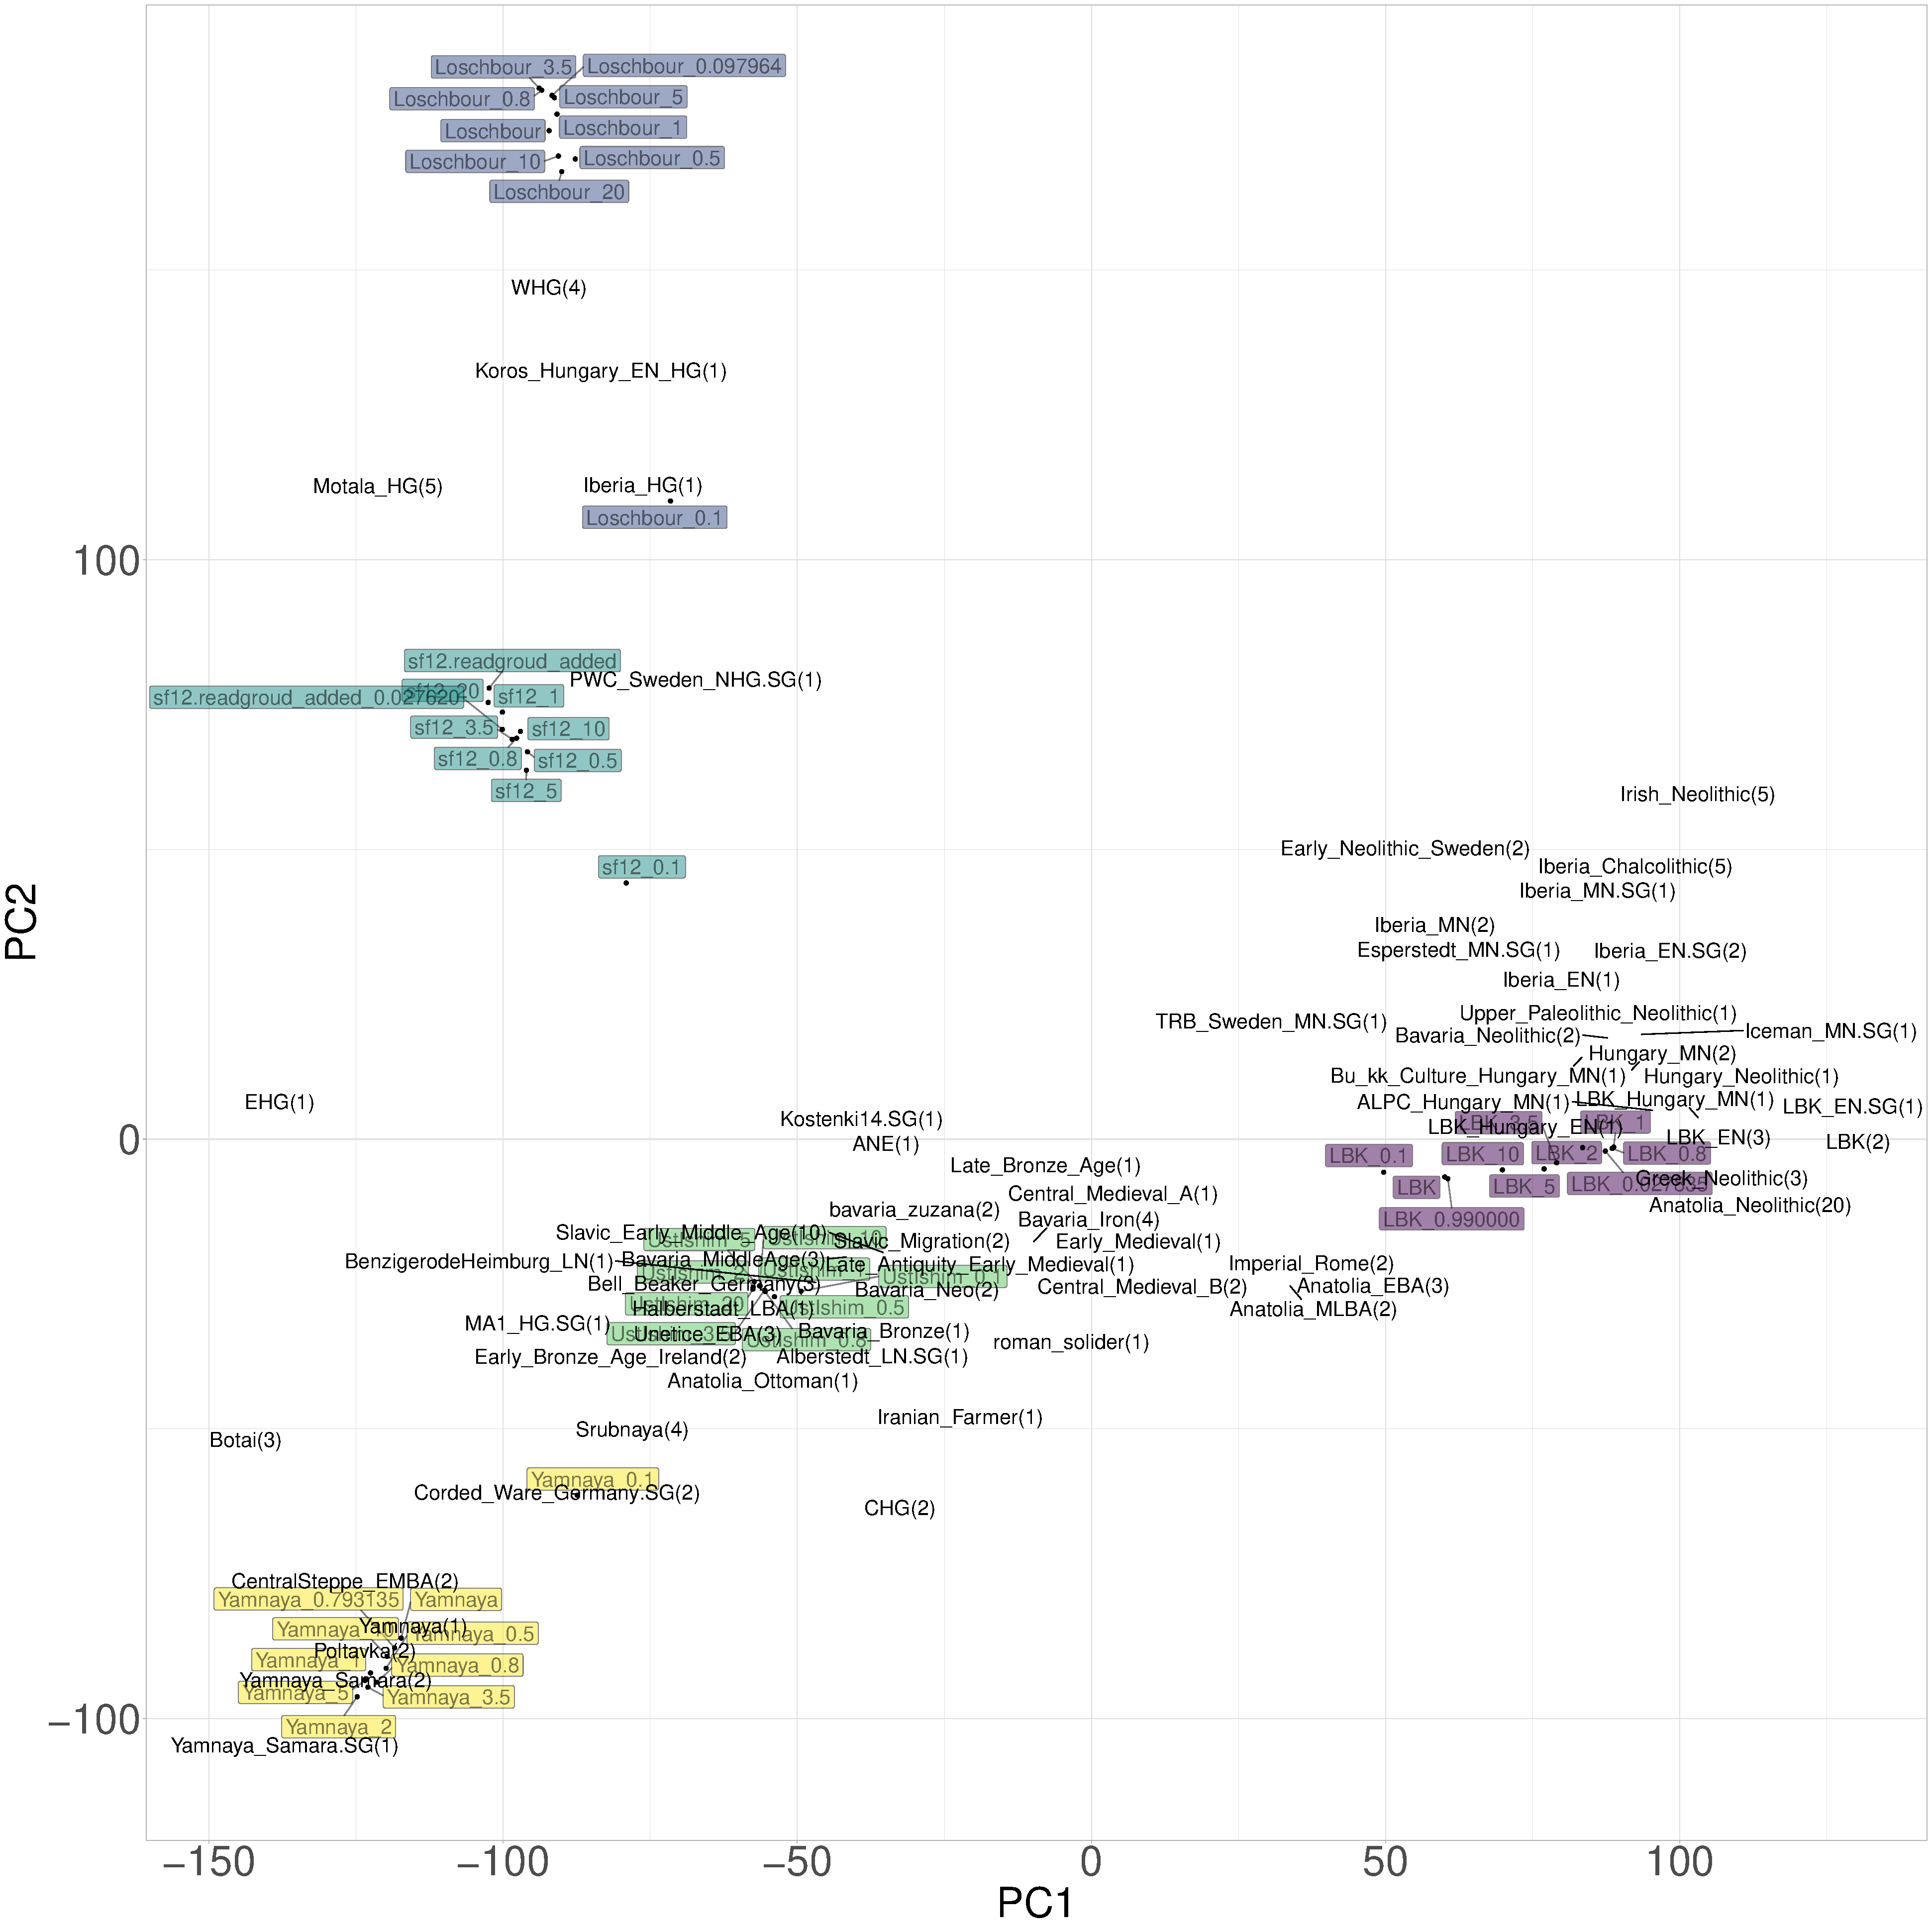
\includegraphics[width=1.0\textwidth]{../images/chapter1/PCA_panel_allInds.allCoverage.pdf}
    \caption{Principle component analysis (PCA) of downsampled, full coverage and downloaded ancient individuals generated from the linked chunklengths matrix. Full coverage and downsampled genomes of the same individual are coloured the same. Reference individuals are grouped into populations plotted as the mean principle components for all individuals within the population. Numbers in labels correspond to the number of individuals within the reference population. 0.1x samples have red border for clarity.}
    \label{fig:PCA_panel_allInds_allCoverage}
\end{figure}

\begin{table}
\centering
\begin{tabular}[t]{lllll}
\toprule
Coverage & Loschbour & sf12 & UstIshim & Yamnaya\\
\midrule
0.1 & Iberia\_HG & PWC\_SwedenNHG.SG & BHeimburg\_LN & CordedWare\\
0.5 & Loschbour & sf12 & UstIshim & Poltavka\\
0.8 & Loschbour & sf12 & UstIshim & Poltavka\\
1 & Loschbour & sf12 & UstIshim & Poltavka\\
2 & Loschbour & sf12 & UstIshim & YamnayaSamara\\
3.5 & Loschbour & sf12 & UstIshim & YamnayaSamara\\
5 & Loschbour & sf12 & UstIshim & YamnayaSamara\\
10 & Loschbour & sf12 & UstIshim & Yamnaya\\
20 & Loschbour & sf12 & UstIshim & Yamnaya\\
\bottomrule
\end{tabular}
\caption{For each downsampled individual at each level of coverage, each entry gives the closest Cartesian neighbour based upon the PCA in Fig \ref{fig:PCA_panel_allInds_allCoverage}, not including other downsamples.}
\label{tab:ClosestNeighbour}
\end{table}


Taken together, this data suggests a minimal effect of coverage down to and including 0.5x mean depth. To my knowledge, no other study has evaluated the effect of coverage on ChromoPainter analysis down to a coverage of 0.5x. Margaryan et al (2020) showed a minimal effect of coverage at 1x and that fineSTRUCTURE groupings, containing individuals as low as 0.5x coverage, were not driven by coverage \cite{margaryan2020population}. 


\subsection{SOURCEFIND}

I next determined the effect of sequencing coverage on the ancestry proportions estimated by SOURCEFIND, which accounts for variable donor group sizes and incomplete lineage sorting  to improve interpretability relative to the raw chunklengths matrix.

I began by considering three ancestral sources, or `surrogates', fixed as Anatolia Neolithic, Western Hunter-Gatherer and Yamnaya steppe pastoralist. I compared inferred proportions for the same individual across different levels of coverage (Fig. \ref{fig:3pop_SF_downsampled}). 

\begin{figure}[htp]
    \centering
    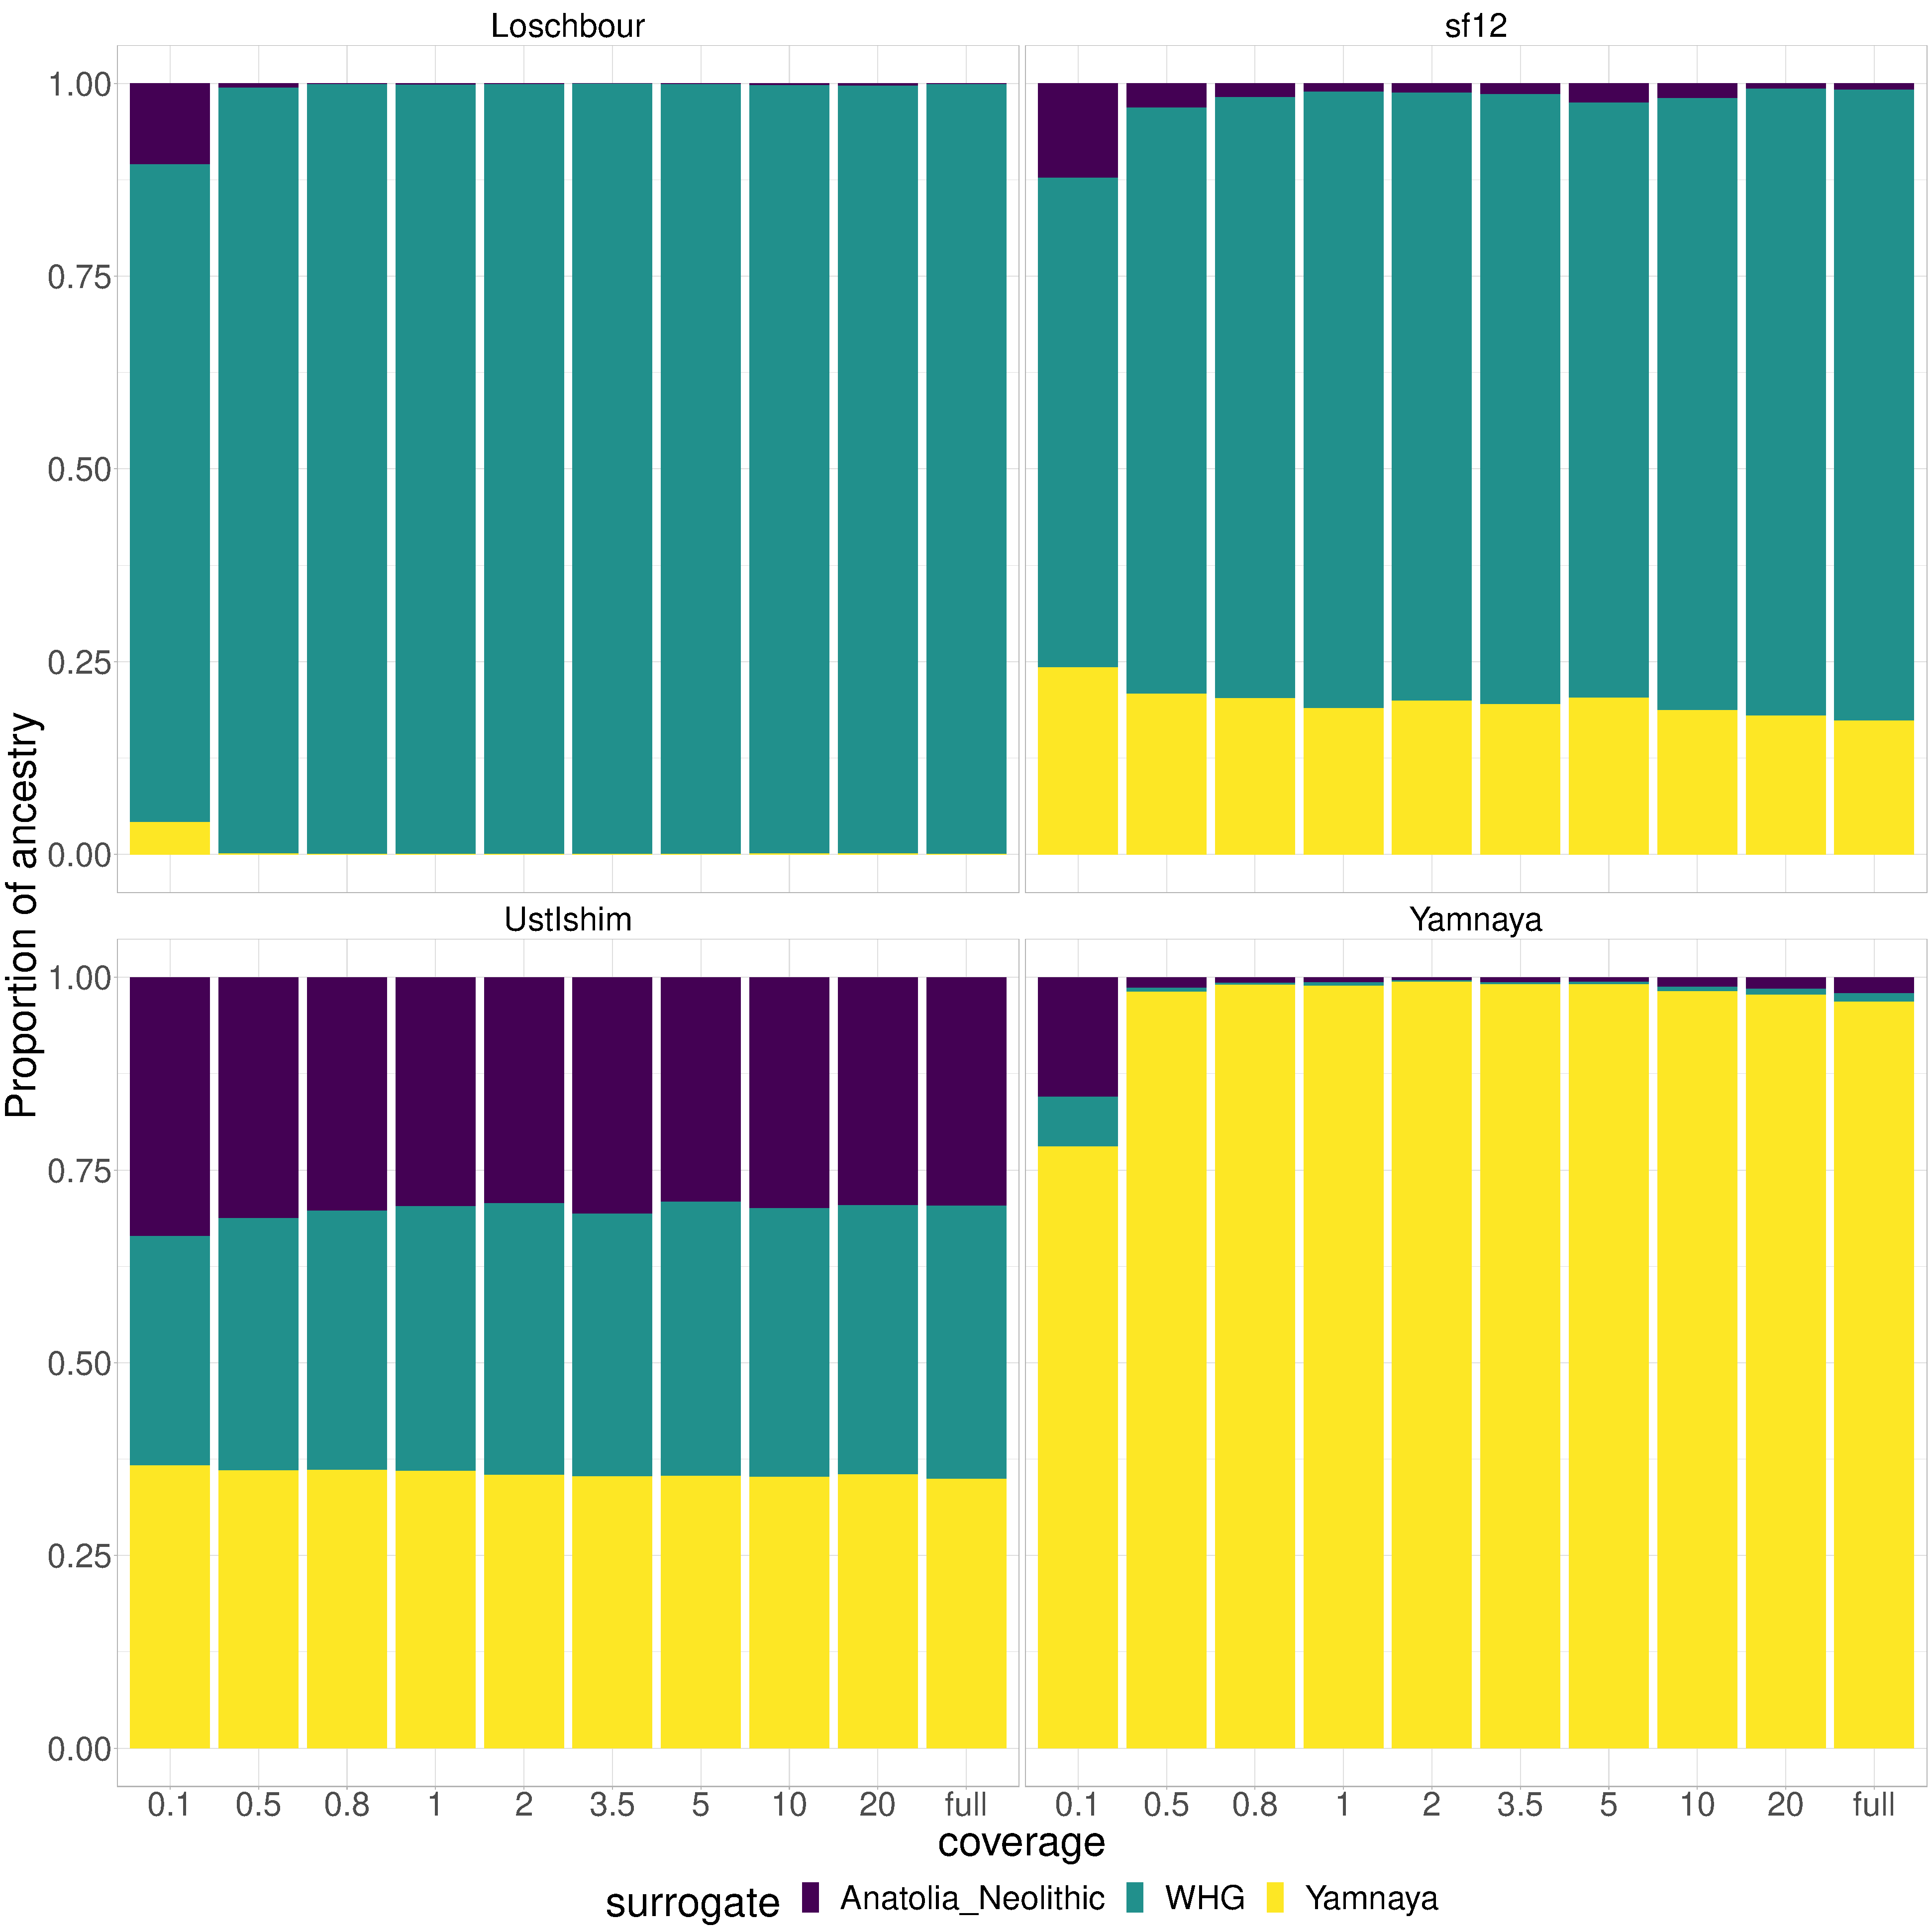
\includegraphics[width=1.0\textwidth]{../images/chapter1/3pop_SF_downsampled.pdf}
    \caption{Each panel gives SOURCEFIND inferred recent ancestry sharing proportions for a different downsampled genome. Bars represent proportion of ancestry, coloured by different surrogates. Different coverages for the same individual are given within each panel. Three surrogates were used.}
    \label{fig:3pop_SF_downsampled}
\end{figure}

Consistent with previous results, SOURCEFIND estimates are robust down to 0.5-0.8x coverage. At 0.1x coverage, there is an increase in ancestry components that are not present in higher coverage samples, suggesting they are artefacts caused by low coverage. For example, small components of Anatolia Neolithic and Yamnaya ancestry appear in Loschbour at 0.1x coverage, which are not present at any higher coverages. Above 0.5x coverage, the effect of coverage on estimated ancestry proportions appears to be marginal. For example, in sf12, the difference in the minor ancestry component of Anatolia Neolithic is, at most, 2.4\%. LBK was excluded because downsamples had anomalously poor results; I inferred roughly equal proportions of all surrogates in spite of the fact that they should have been almost 100\% farmer. 

However, more than three surrogates are often used, as SOURCEFIND is meant to infer the most important contributors without \textit{a priori} knowledge of the samples' ancestry. Therefore, I re-ran SOURCEFIND using 39 surrogate populations (Fig. \ref{fig:SOURCEFIND_AllPSop_downsampled}). For all downsamples above 0.1x in coverage, the ordering of proportions for each surrogate was the same. 

\begin{figure}[htp]
    \centering
    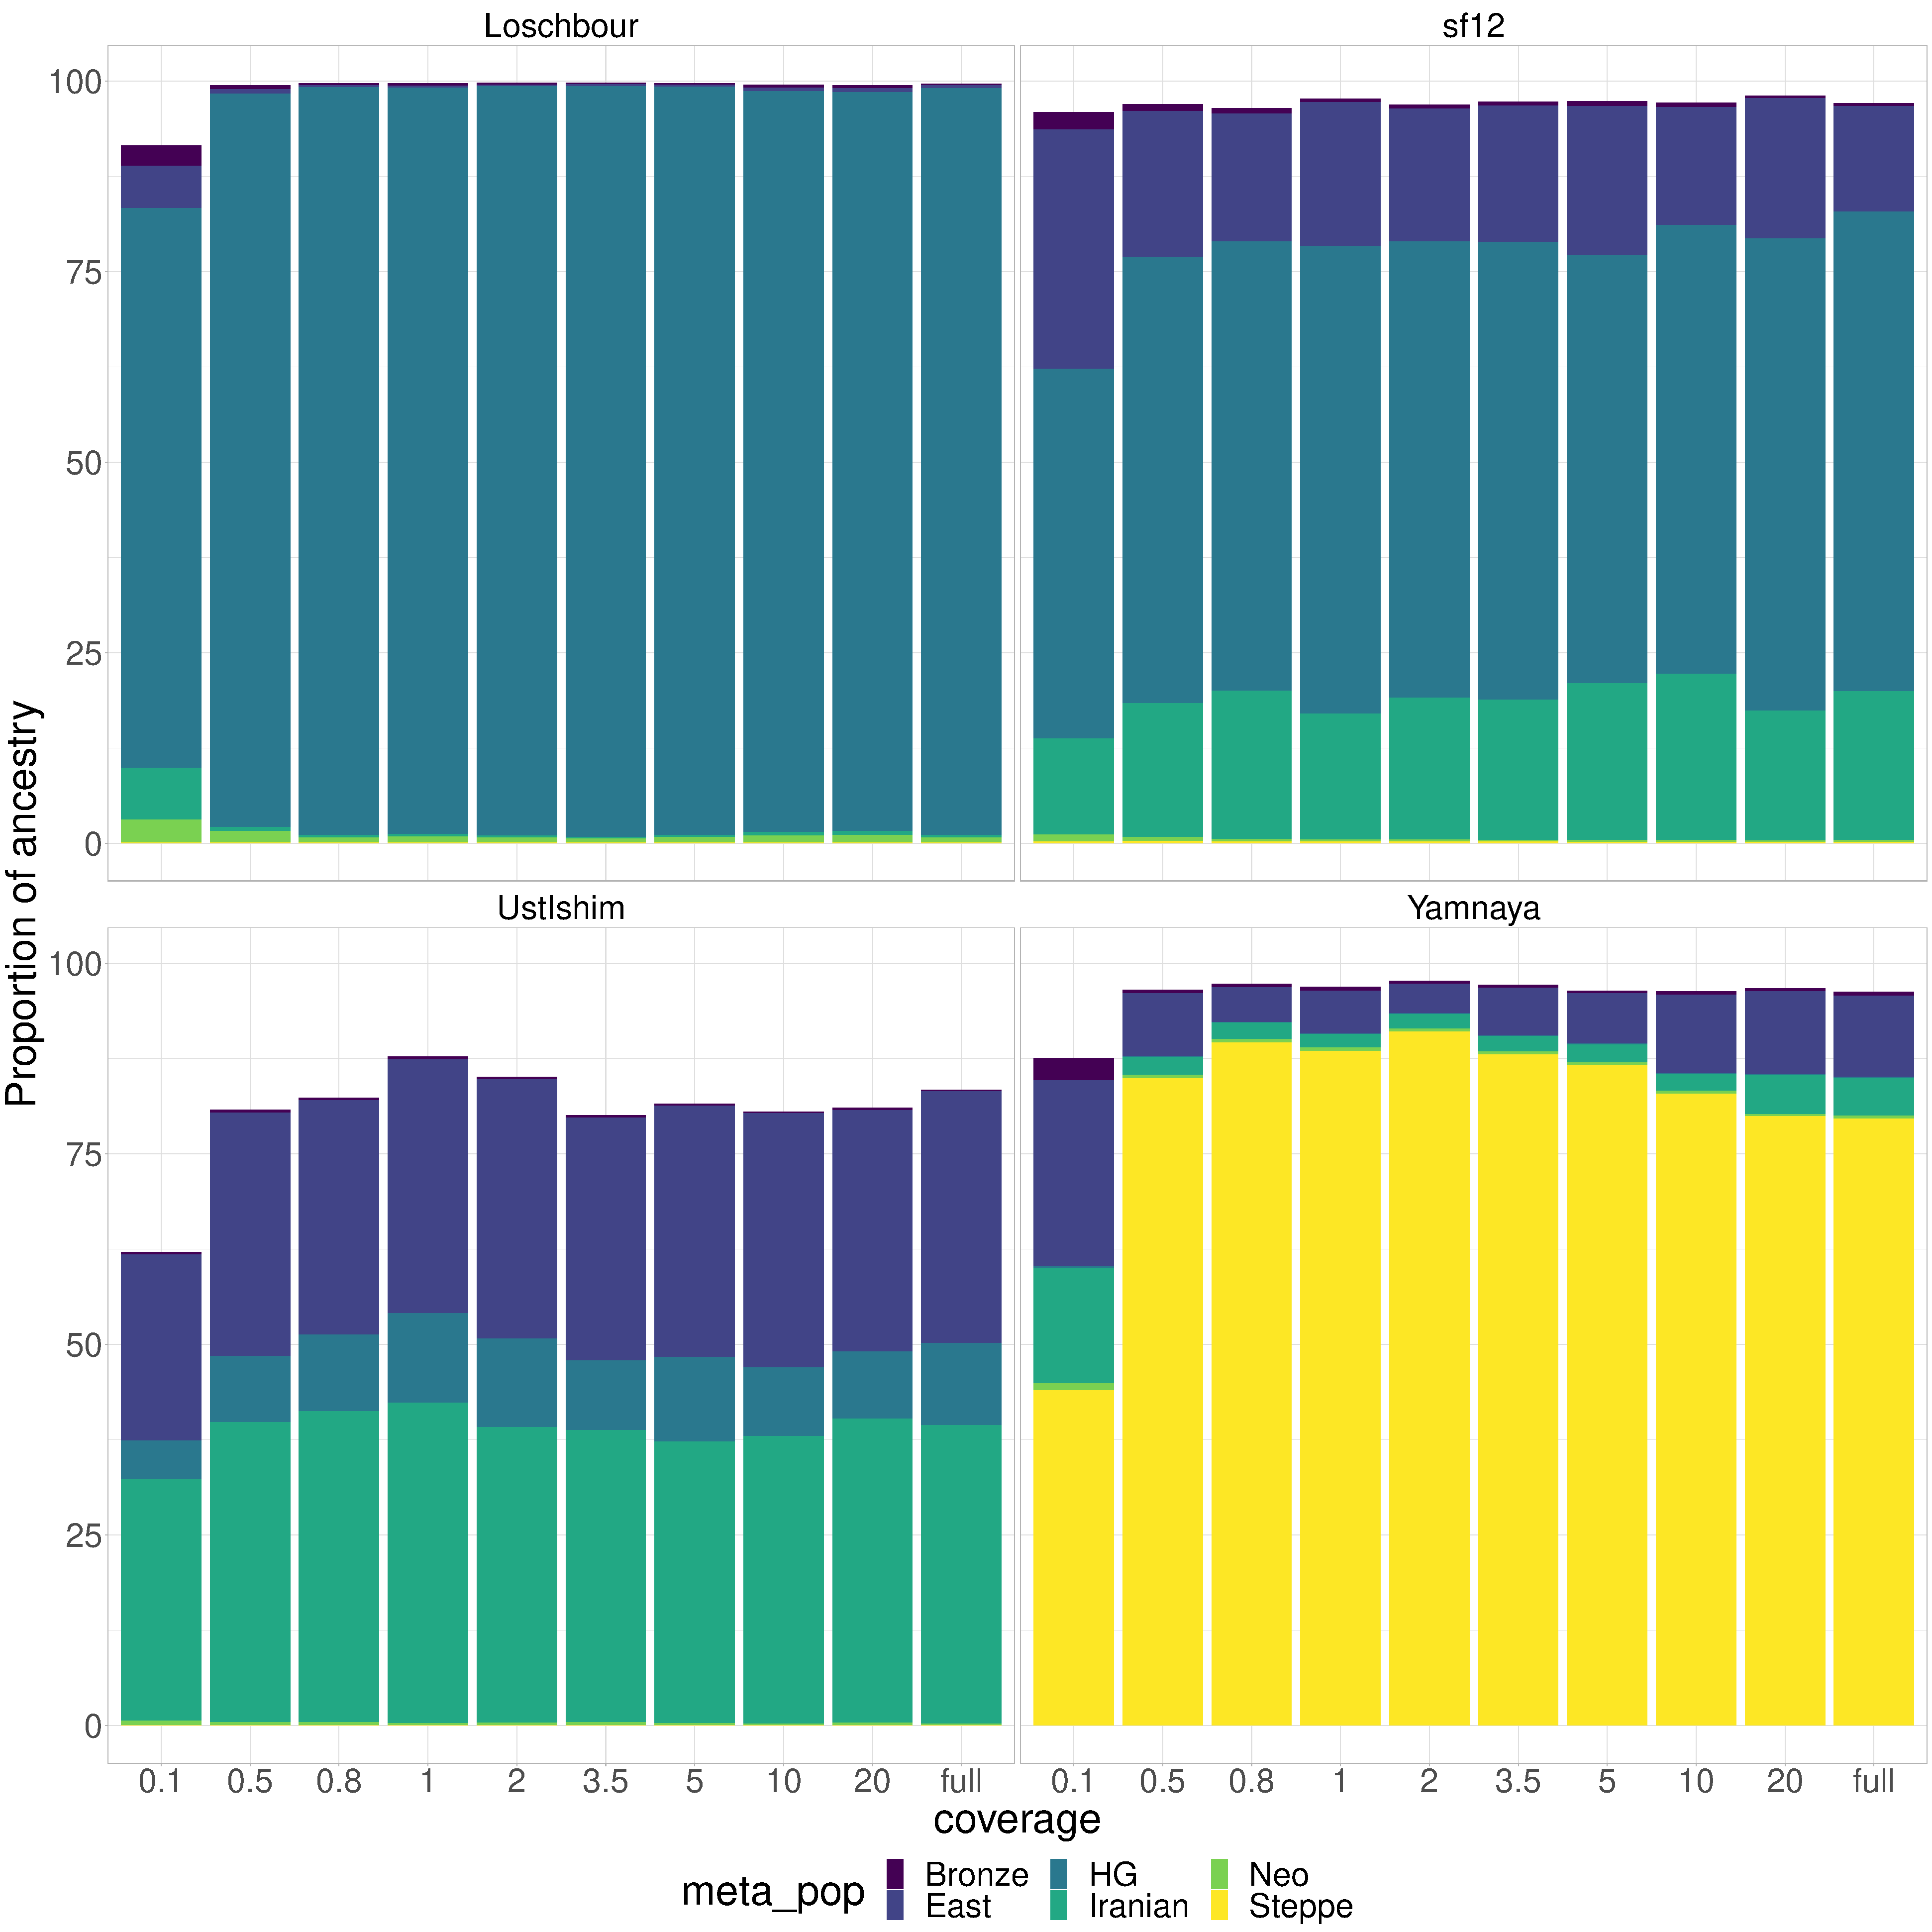
\includegraphics[width=1.0\textwidth]{../images/chapter1/Allpops_SF_downsampled.pdf}
    \caption{Each panel gives information for a different downsampled genome. Bars represent proportion of ancestry inferred by SOURCEFIND, coloured by different surrogates. Different coverages for the same individual are given within each panel. All 39 ancient surrogates were used. Only surrogates with more than 5\% are shown. Ancient surrogates grouped into hand-assigned `meta-populations' for visual clarity. LBK excluded because of anomalously poor results.}
    \label{fig:SOURCEFIND_AllPSop_downsampled}
\end{figure}

Again, Loschbour seems to be the least affected by coverage, with only slight differences between the 0.5x and full coverage samples. It is known that Upper Palaeolithic / Early Neolithic Hunter-Gatherer populations were small and lacked genetic diversity \cite{excoffier1999hunter, Lazaridis2014, Fu2016}. It is therefore expected that Hunter-Gatherers would share longer IBD segments than individuals from outbred populations. Accordingly, this may make estimating SOURCEFIND proportions easier.


\section{Issues and possible solutions for low coverage ancient DNA}

The previous section outlined a drawback of performing ChromoPainter analysis on low coverage ($<$0.5x) ancient DNA samples; low coverage samples appear to be shifted towards the origin of a principle component analysis (PCA) relative to the same sample at higher coverage (Fig. \ref{fig:PCA_panel_allInds_allCoverage}) and can contain ancestry estimates that are not present in the same full coverage sample (Fig. \ref{fig:3pop_SF_downsampled}).  This is evident for the lowest coverage samples at 0.1x and suggests that samples of this coverage cannot be reliably analysed using         current methodology.

In order to solve the issue of coverage-related bias, it is first necessary to determine at which stage of the analysis pipeline the bias is introduced. By `analysis pipeline', I refer to the three stages of (1) variant calling, (2) imputation and phasing, and (3) ChromoPainter described in the methods section.

\subsection{PCA imputation test} \label{sec:PCAImputationTest}

To explicitly test at what stage the bias is introduced, I performed a set of principle component analyses on the downsampled data. First, I performed PCA projections of all downsampled ancient individuals onto a set of present-day European individuals (shown in Table \ref{tab:HB_pops}) using i) pre-GLIMPSE genotypes and ii) post-GLIMPSE (imputed) genotypes (Fig. \ref{fig:pre_GLIMPSE_PCA}). PCA projections are used when the target dataset, in this case downsampled ancients, contain variable levels of missing data.  

The results show that there is no apparent coverage-related bias in the pre-GLIMPSE PCA; the 0.1x samples do not substantially differ in their position from the other downsamples of the same individual. However, there is a degree of noise; for example, the LBK downsamples are spread over a small region on the PCA. 

On the other hand, downsamples of UstIshim, sf12 and Loschbour are shifted to the centre of the post-GLIMPSE PCA and away from the full coverage individual and other downsamples. This suggests that coverage-related bias is being introduced in the imputation stage. At the same time, GLIMPSE appears to have removed some of the noise in the downsampled individuals of coverage $\geq$0.5x. For instance, the noise observed in the LBK samples in the pre-imputation PCA is substantially reduced and the samples cluster more tightly.  

I also performed PCAs based upon an all-v-all ChromoPainter painting using the same set of present-day European samples (Table \ref{tab:HB_pops}) and downsampled ancient individuals as previously, in both linked and unlinked modes. There is an increased amount of noise and evidence of coverage-related bias relative to the post-GLIMPSE genotype PCA. Fig. \ref{fig:CP_linked_unlinked}) displays the PCA for the same painting, but using the unlinked chunkcounts matrix. Comparing the linked and unlinked PCAs shows the effect of including linkage (i.e. haplotype information) on the amount of bias and noise across each sample. Per-sample, there appears to be reduced noise in the unlinked painting.

These results suggest that imputation using GLIMPSE introduces a degree of bias into 0.1x samples that is not apparent on non-imputed genotypes. They also suggest that ChromoPainter introduces an additional degree of bias when analysing haplotypes, or that it amplifies bias already present introduced at the imputation stage. Accordingly, removing SNPs which have been poorly imputed may be a way to mitigate such biases.

\begin{figure}[htp]
    \centering
    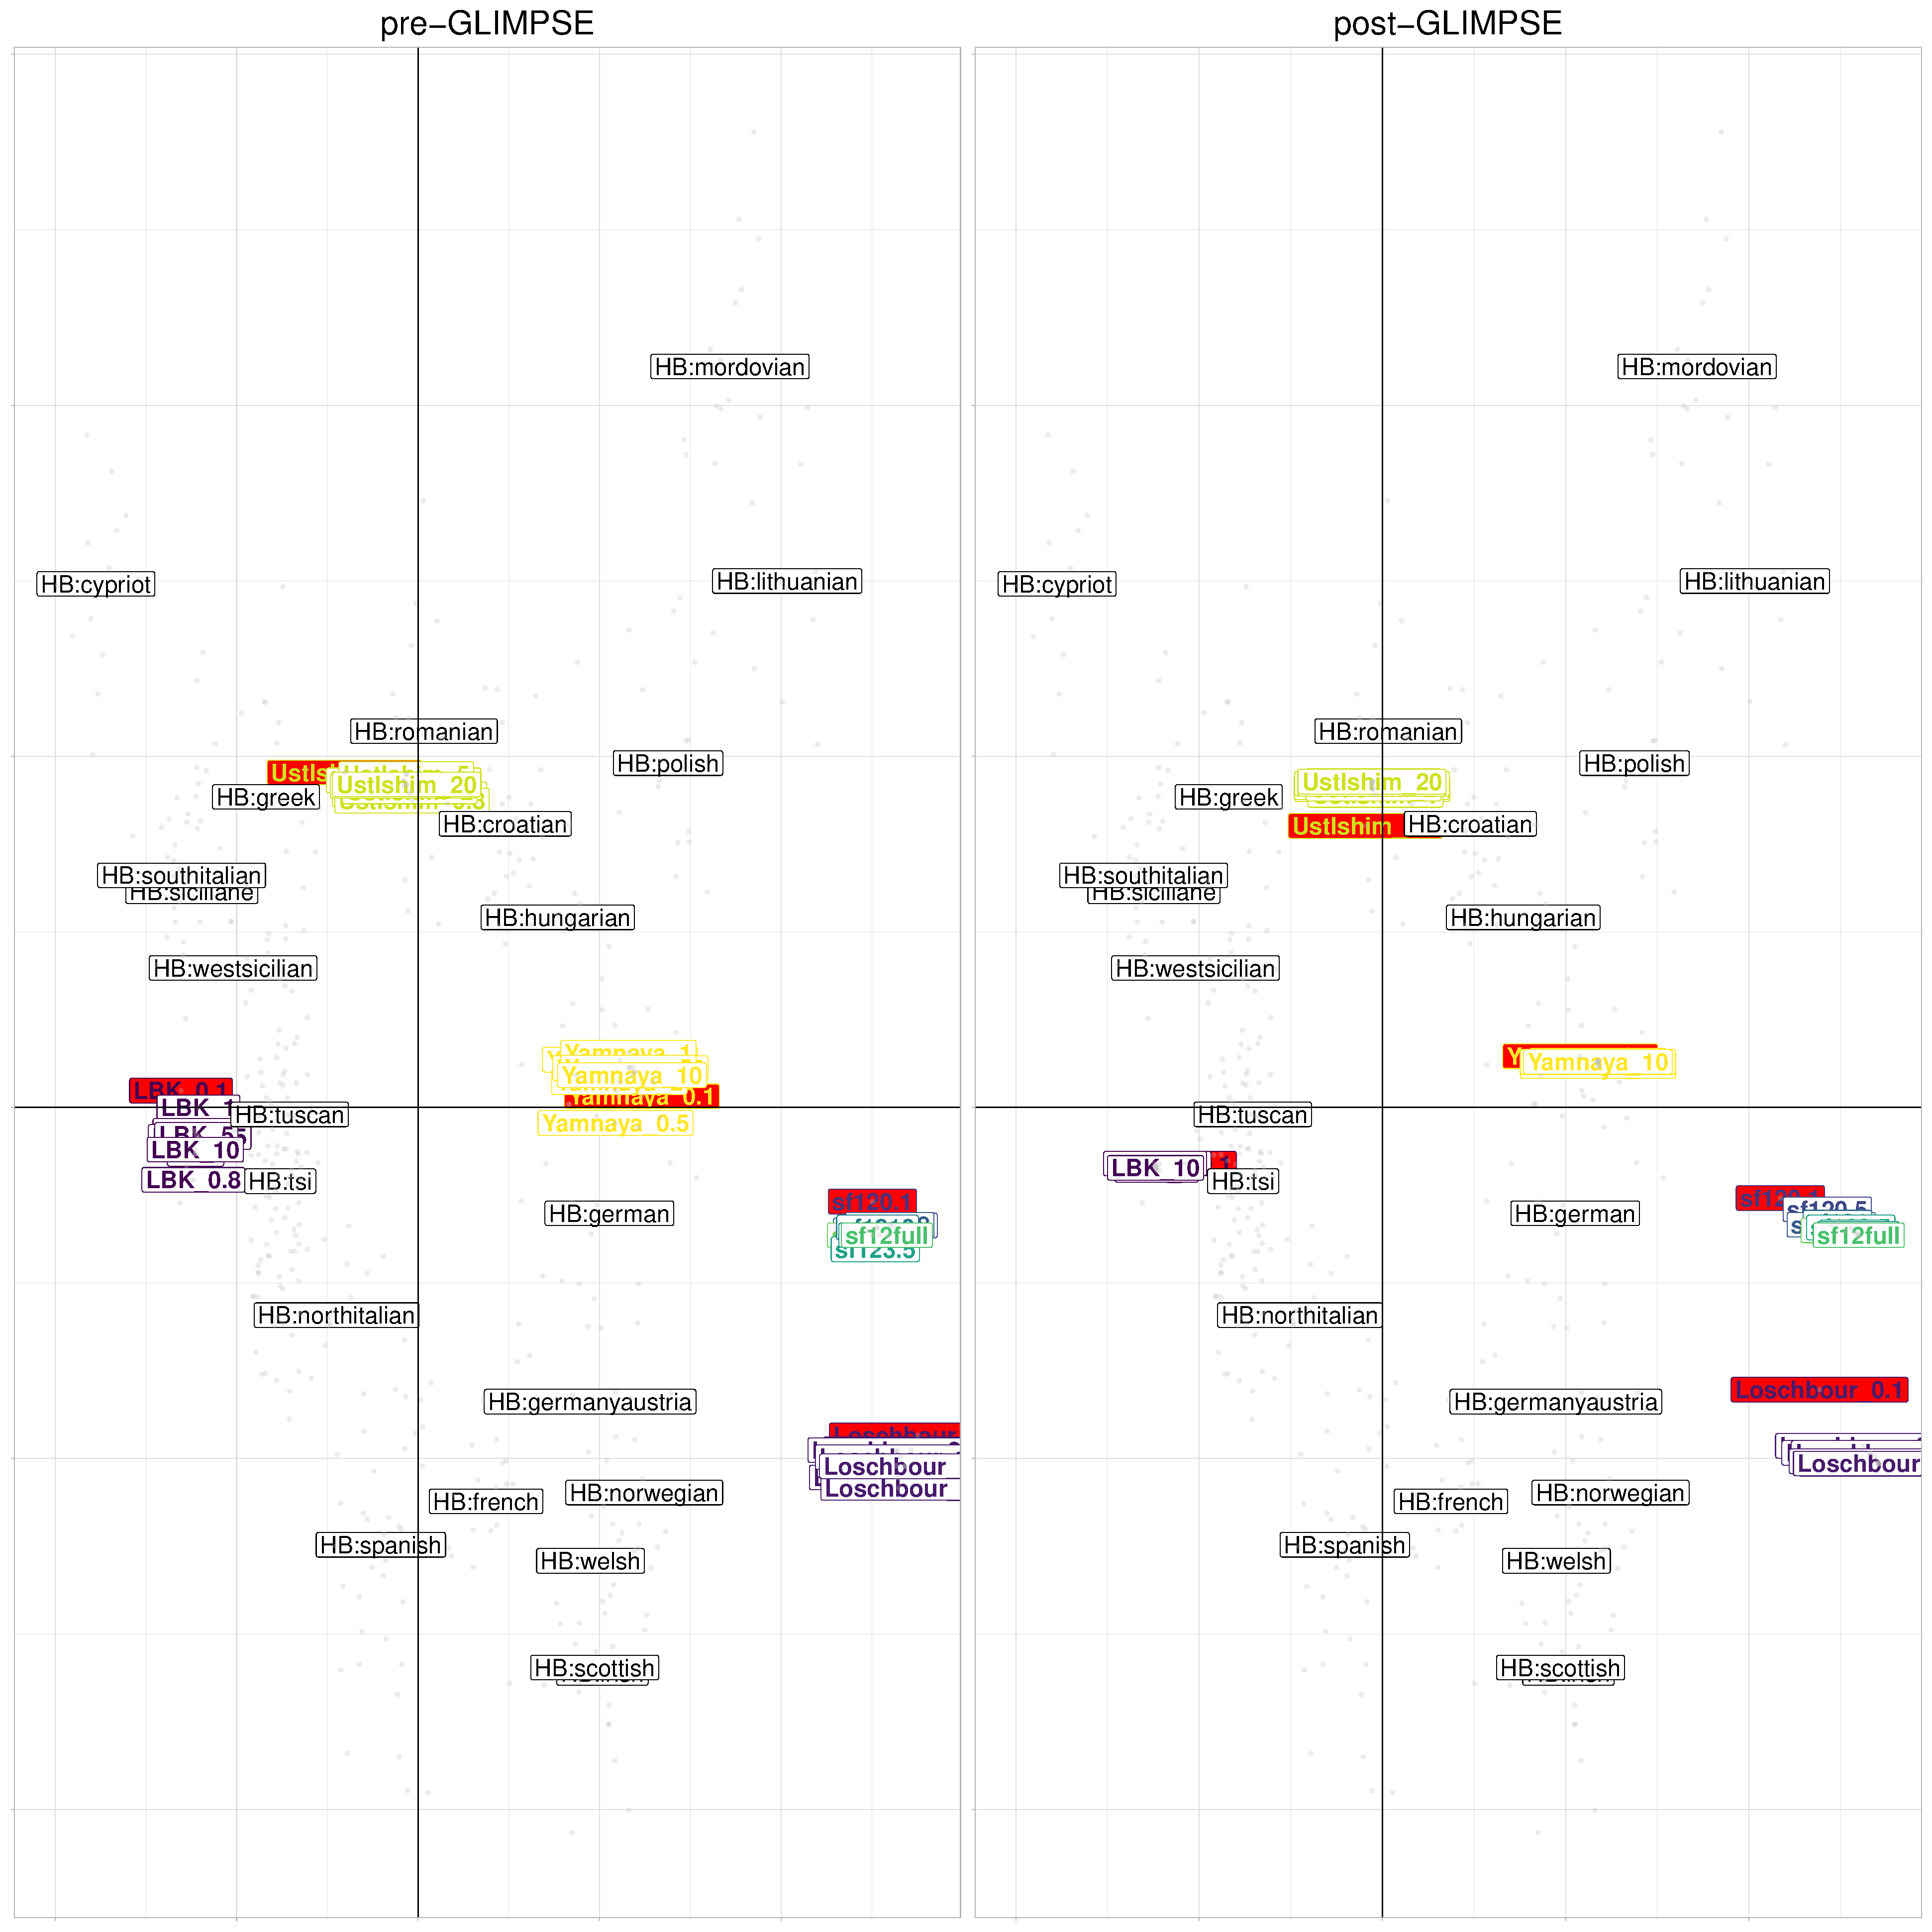
\includegraphics[width=1.0\textwidth]{../images/chapter1/pre_post_GLIMPSE_PCA.pdf}
    \caption{Principle Component Analysis. Left - pre-GLIMPSE genotypes. Right - post-GLIMPSE (imputed) genotypes. White labels correspond to the midpoint of all samples from that population, grey points correspond to modern individuals. 0.1x samples highlighted in red for clarity. Black lines are $y=0; x=0$.}
    \label{fig:pre_GLIMPSE_PCA}
\end{figure}

\begin{figure}[htp]
    \centering
    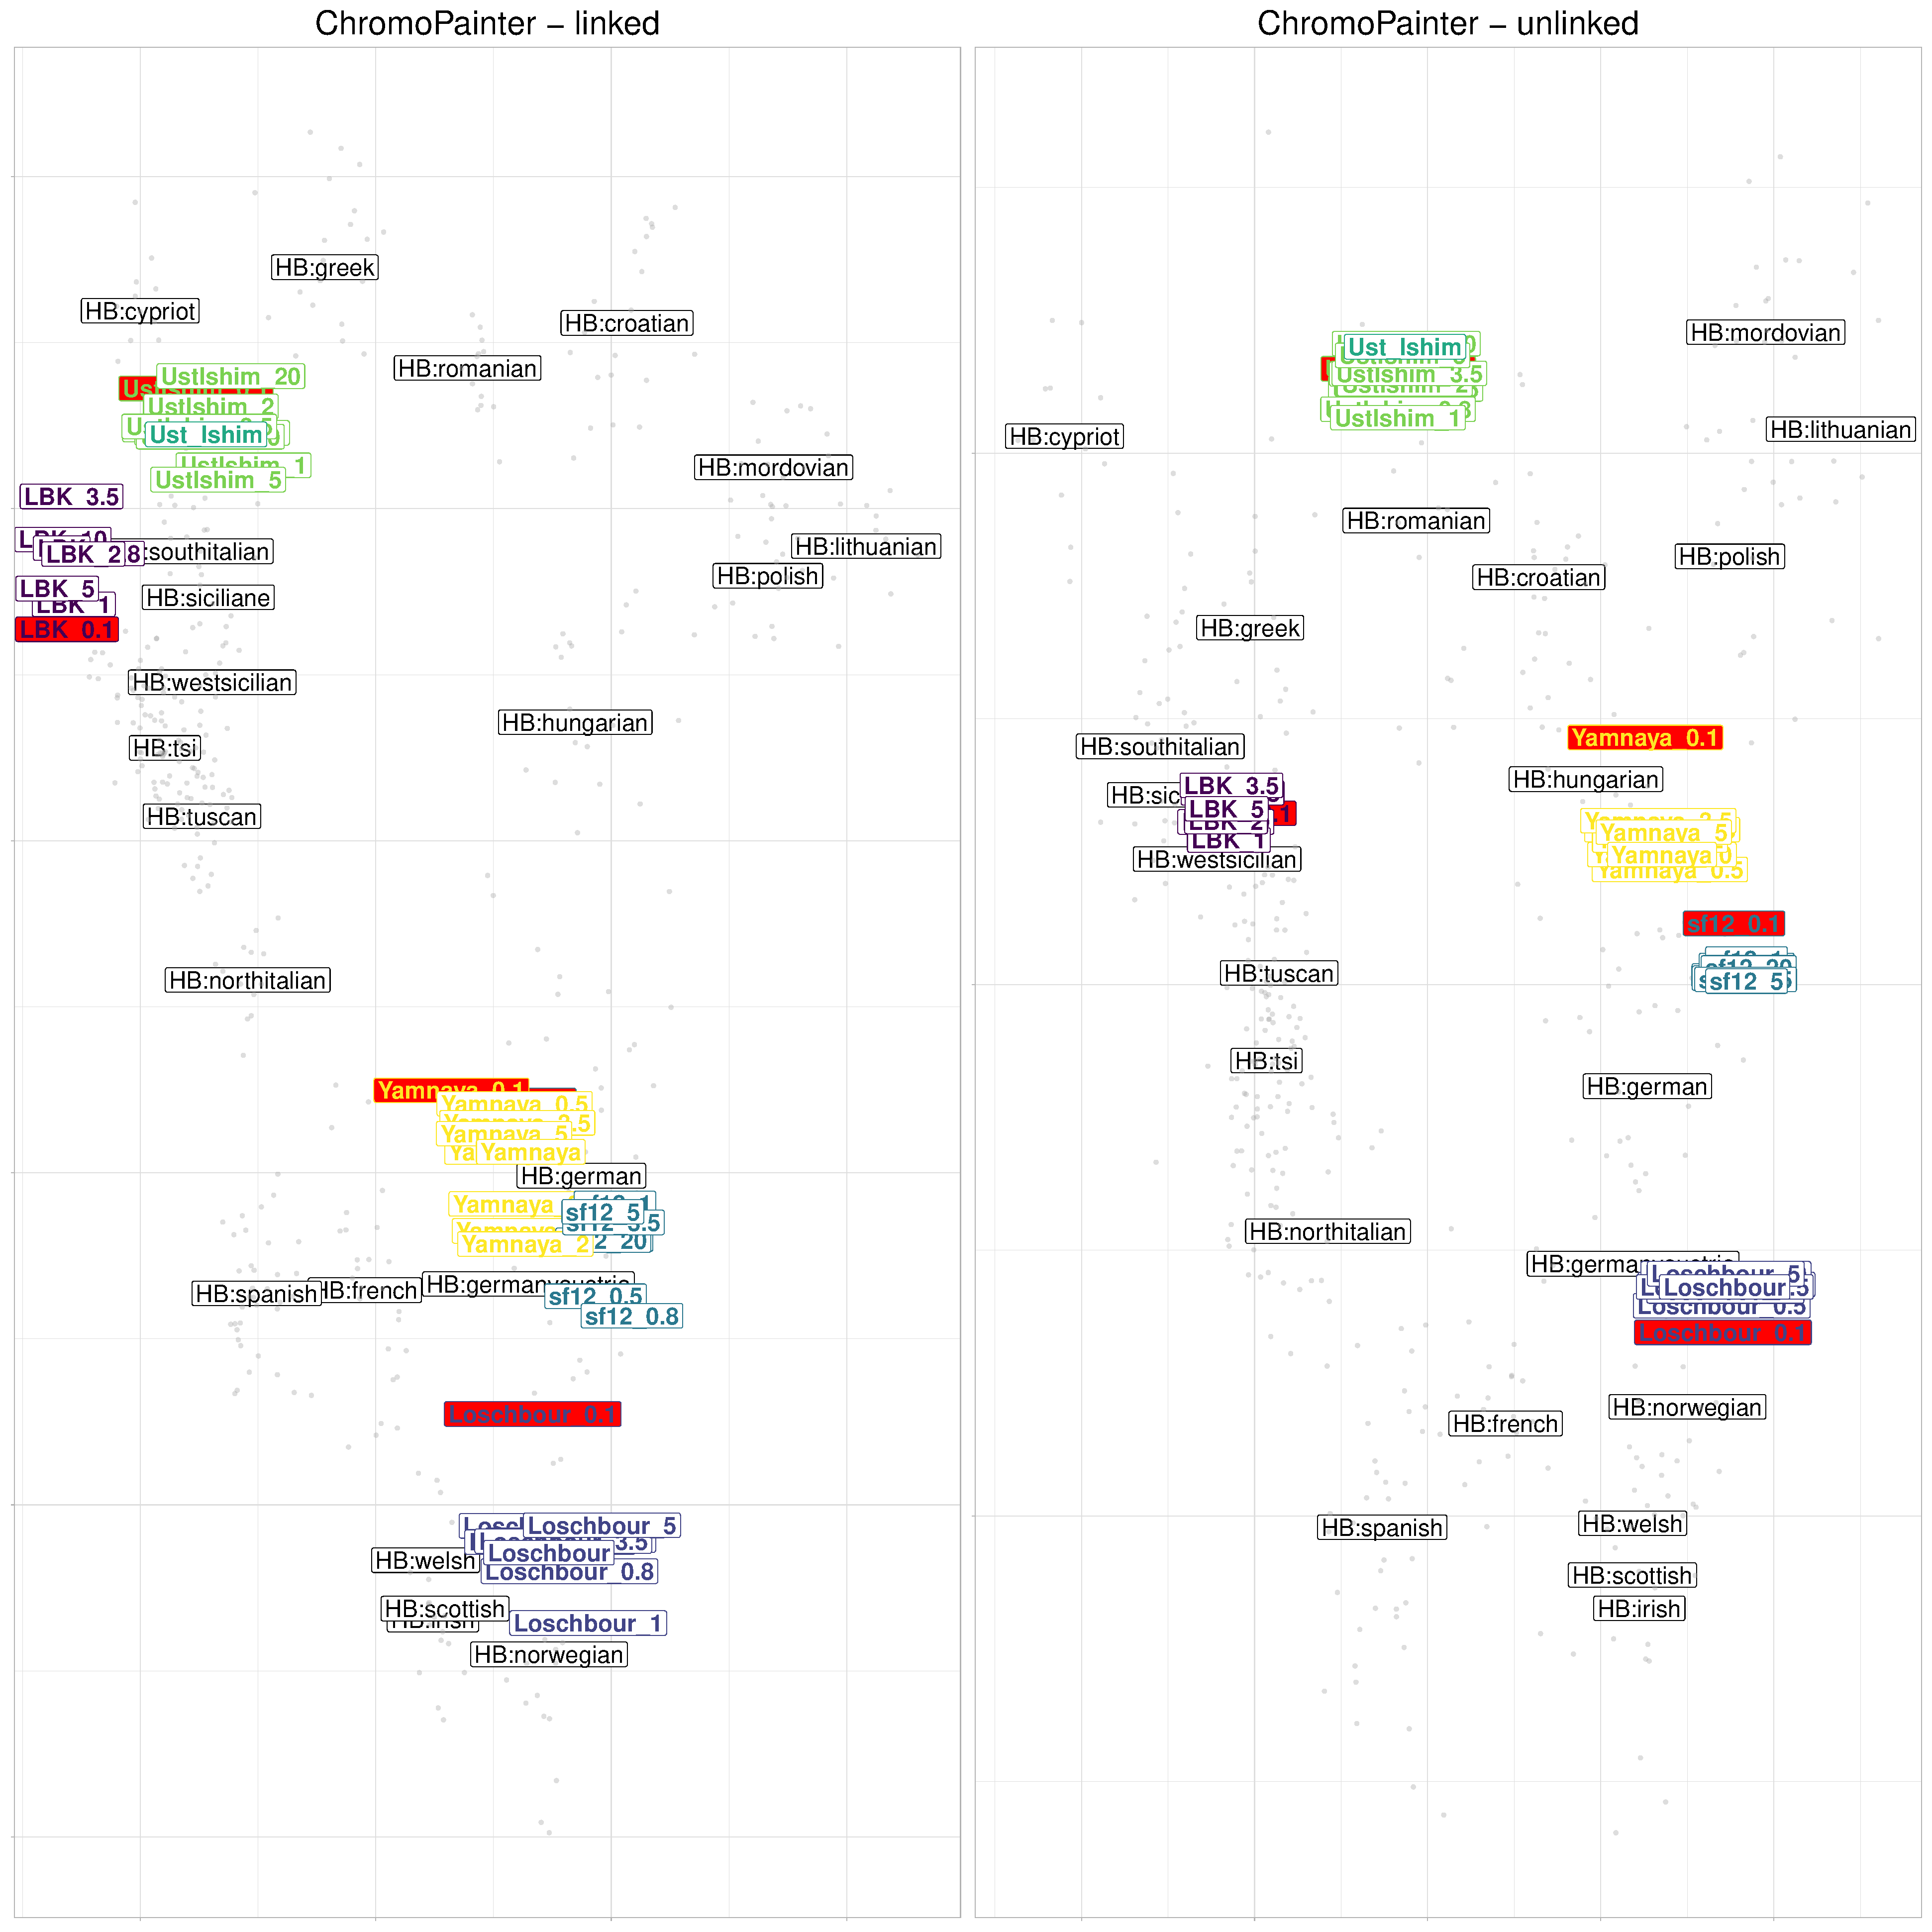
\includegraphics[width=1.0\textwidth]{../images/chapter1/CP_linked_unlinked.pdf}
    \caption{Left - ChromoPainter Linked. Right - ChromoPainter Unlinked. White labels correspond to the midpoint of all samples from that population, grey points correspond to modern individuals. 0.1x samples highlighted in red for clarity. Black lines are $y=0; x=0$.}
    \label{fig:CP_linked_unlinked}
\end{figure}

\subsection{Direct imputation test} \label{DirectImputationTest}

The previous section suggested that imputation plays a role in the introduction of coverage-related bias. However, it is not clear whether it is `bias', i.e.\ towards the reference population used to assist imputation, or `noise' due to random incorrect imputation. To directly test whether the effect of imputation is noise or bias, I used the Human Origins dataset (described in Appendix section \ref{HumanOriginsAppendix}), containing the genotypes of 5998 present-day individuals from across the world at 560,442 SNPs. I chose to use present-day samples because there is a larger total number of individuals and larger number of individuals per population, giving more power to detect any potential bias. Additionally, the populations in present-day samples are more homogenous and well-defined compared to ancient groups. I set all but 70,000 random SNPs as missing and imputed missing positions using the HRC as a reference, in order to simulate a dataset where the majority of SNPs are imputed. I then performed an all-v-all painting of i) the original Human Origins dataset where none of the 560,442 SNPs had been imputed and ii) the simulated dataset where 430,000 SNPs had been imputed. 

Bias occurs when missing genotypes are incorrectly imputed with variants from certain populations more frequently than others. We might expect these populations to be those which are more prevalent in the reference panel. We would correspondingly expect bias to mean that, when painted, some donor populations would donate more than others, relative to if no imputation had taken place. On the other hand, if `noise' is dominating results, we would expect the incorrectly imputed genotypes to be randomly distributed across populations, and similarly we would not expect to see any populations donating more than others relative to if no imputation had taken place. 

Therefore, we can compare the amount different donor groups donate under the dataset where none of the 560,442 SNPs had been imputed versus the dataset where 430,000 (86\%) of these SNPs have been imputed by plotting the mean amount donated by each population using imputed SNPs and non-imputed SNPs (Fig. \ref{fig:imputed_nonimputed_donation}). The 20 populations that contribute most are either European or Jewish. Notably, the Haplotype Reference Consortium panel that was used to impute the data consists primarily of individuals of European descent. The two populations which are over-copied the most after imputation are two English populations from Kent and Cornwall. This suggests that there is a most likely a bias towards copying more from European populations when the data has been imputed using the HRC. 

\begin{figure}[htp]
    \centering
    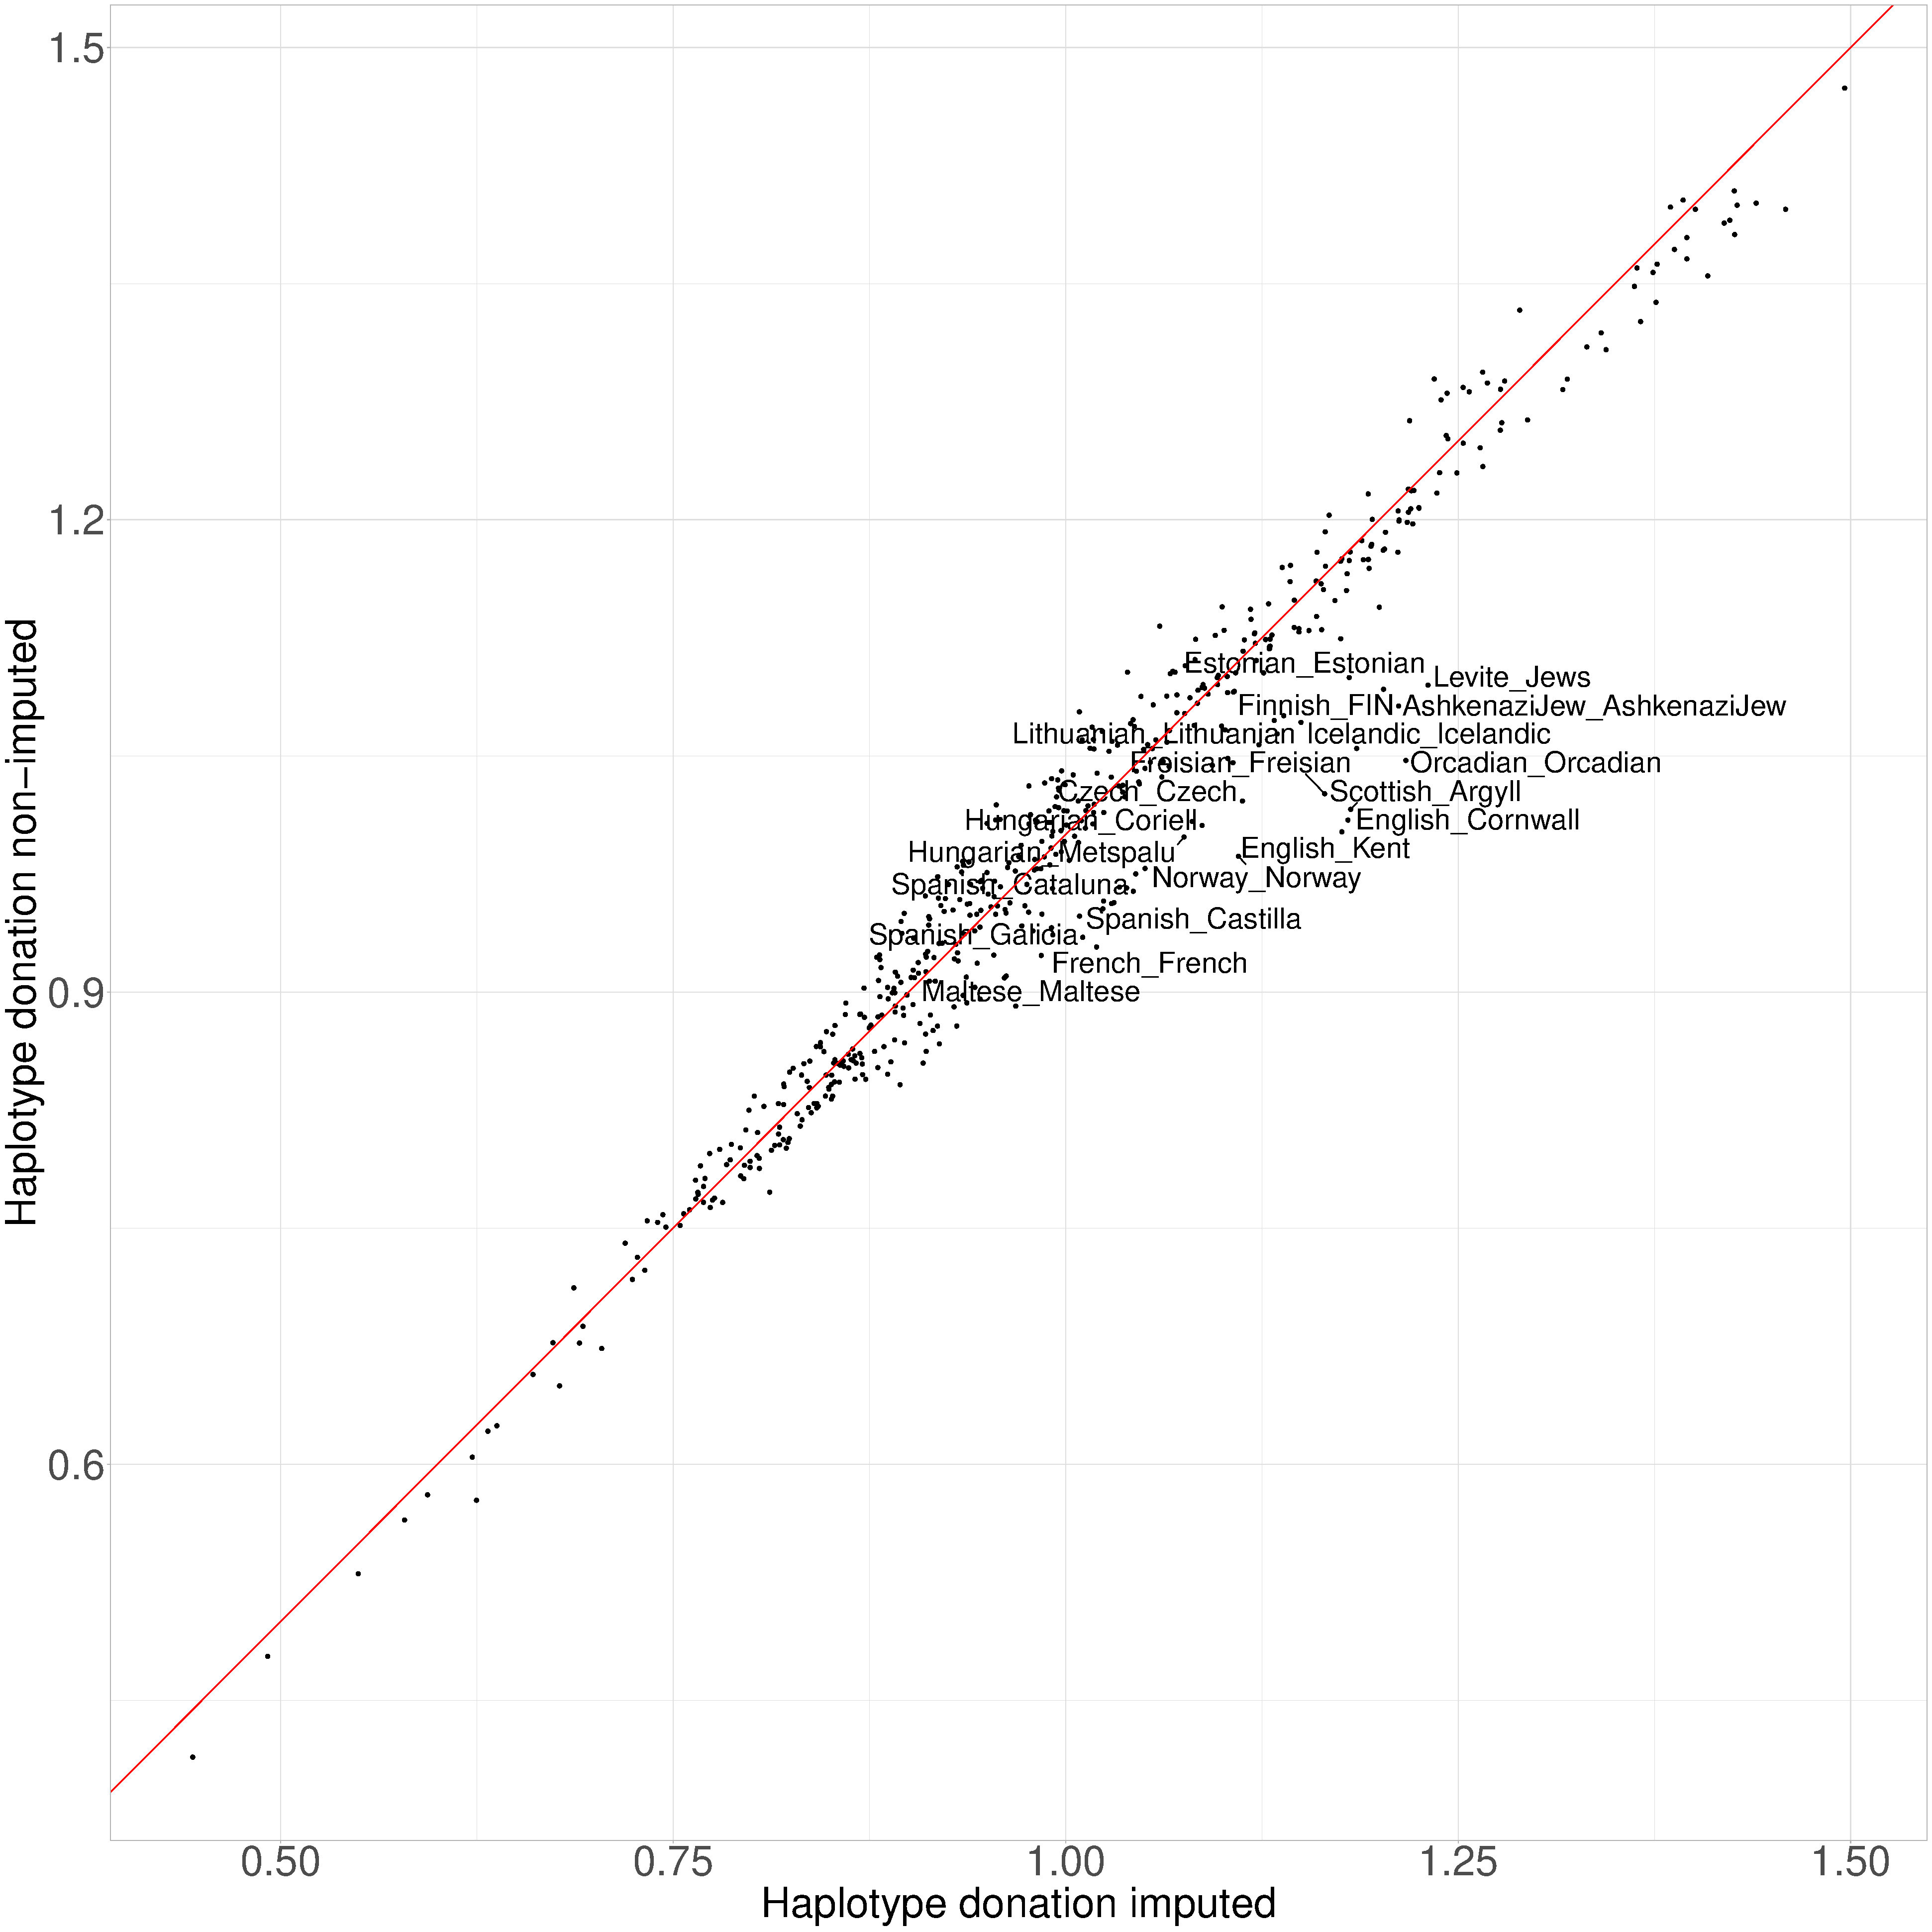
\includegraphics[width=1.0\textwidth]{../images/chapter1/donation_imputed_nonimputed.pdf}
    \caption{Comparison of the mean normalised cM donated by each donor population using the imputed and non-imputed SNP sets. The 20 populations with the largest difference between imputed and non-imputed donation are highlighted. Red line is line of $y=x$.}
    \label{fig:imputed_nonimputed_donation}
\end{figure}

\section{Solutions} \label{sec:Solutions}

In this section I will explore potential solutions to the issue of coverage-related bias. Based on the findings in previous sections, imputation causes bias towards particular reference populations in modern samples.  

\subsection{Accounting for allele likelihoods}

Section \ref{sec:DescriptionChromoPainterV2Uncertainty} describes an improvement to the ChromoPainter algorithm. Instead of assuming that each allele on a haplotype is correct with a probability $1-\theta$, where $\theta$ represents an error probability, the posterior genotype probability from GLIMPSE is accounted for in the emission probabilities of the copying model. The motivation behind this update is that the uncertainty associated with genotype calls at low coverage is suitably propagated throughout the painting process, resulting in uncertain alleles contributing less towards the expected copying values than more certain ones. This is similar in spirit to that of Viera et al (2016), who account for genotype likelihoods to infer inbreeding IBD tracts from low coverage sequencing data \cite{vieira2016estimating}.

To determine whether accounting for allele likelihoods improved the painting accuracy of a low-coverage genome, I painted the individuals downsampled to 0.1x and 0.5x and corresponding full coverage samples using the `standard set' of ancient reference individuals, using both ChromoPainterV2 and ChromoPainterV2Uncertainty. I then calculated Pearson's correlation between the copyvectors of full coverage and downsampled individuals using the two different methods (Fig. \ref{fig:uncertainty_v_noUncertainty_0.5x_0.1x}). This shows that at 0.1x, the ChromoPainterV2 method clearly outperforms ChromoPainterV2Uncertainty across all samples, whereas at 0.5x, the new method marginally outperforms the standard method. Therefore, while accounting for allele likelihoods may improve performance in cases of coverage $\geq$0.5x, which has been shown to still capture some haplotype information, it does not help in cases of coverage of 0.1x where bias problems persist.


\begin{figure}[htp]
    \centering
    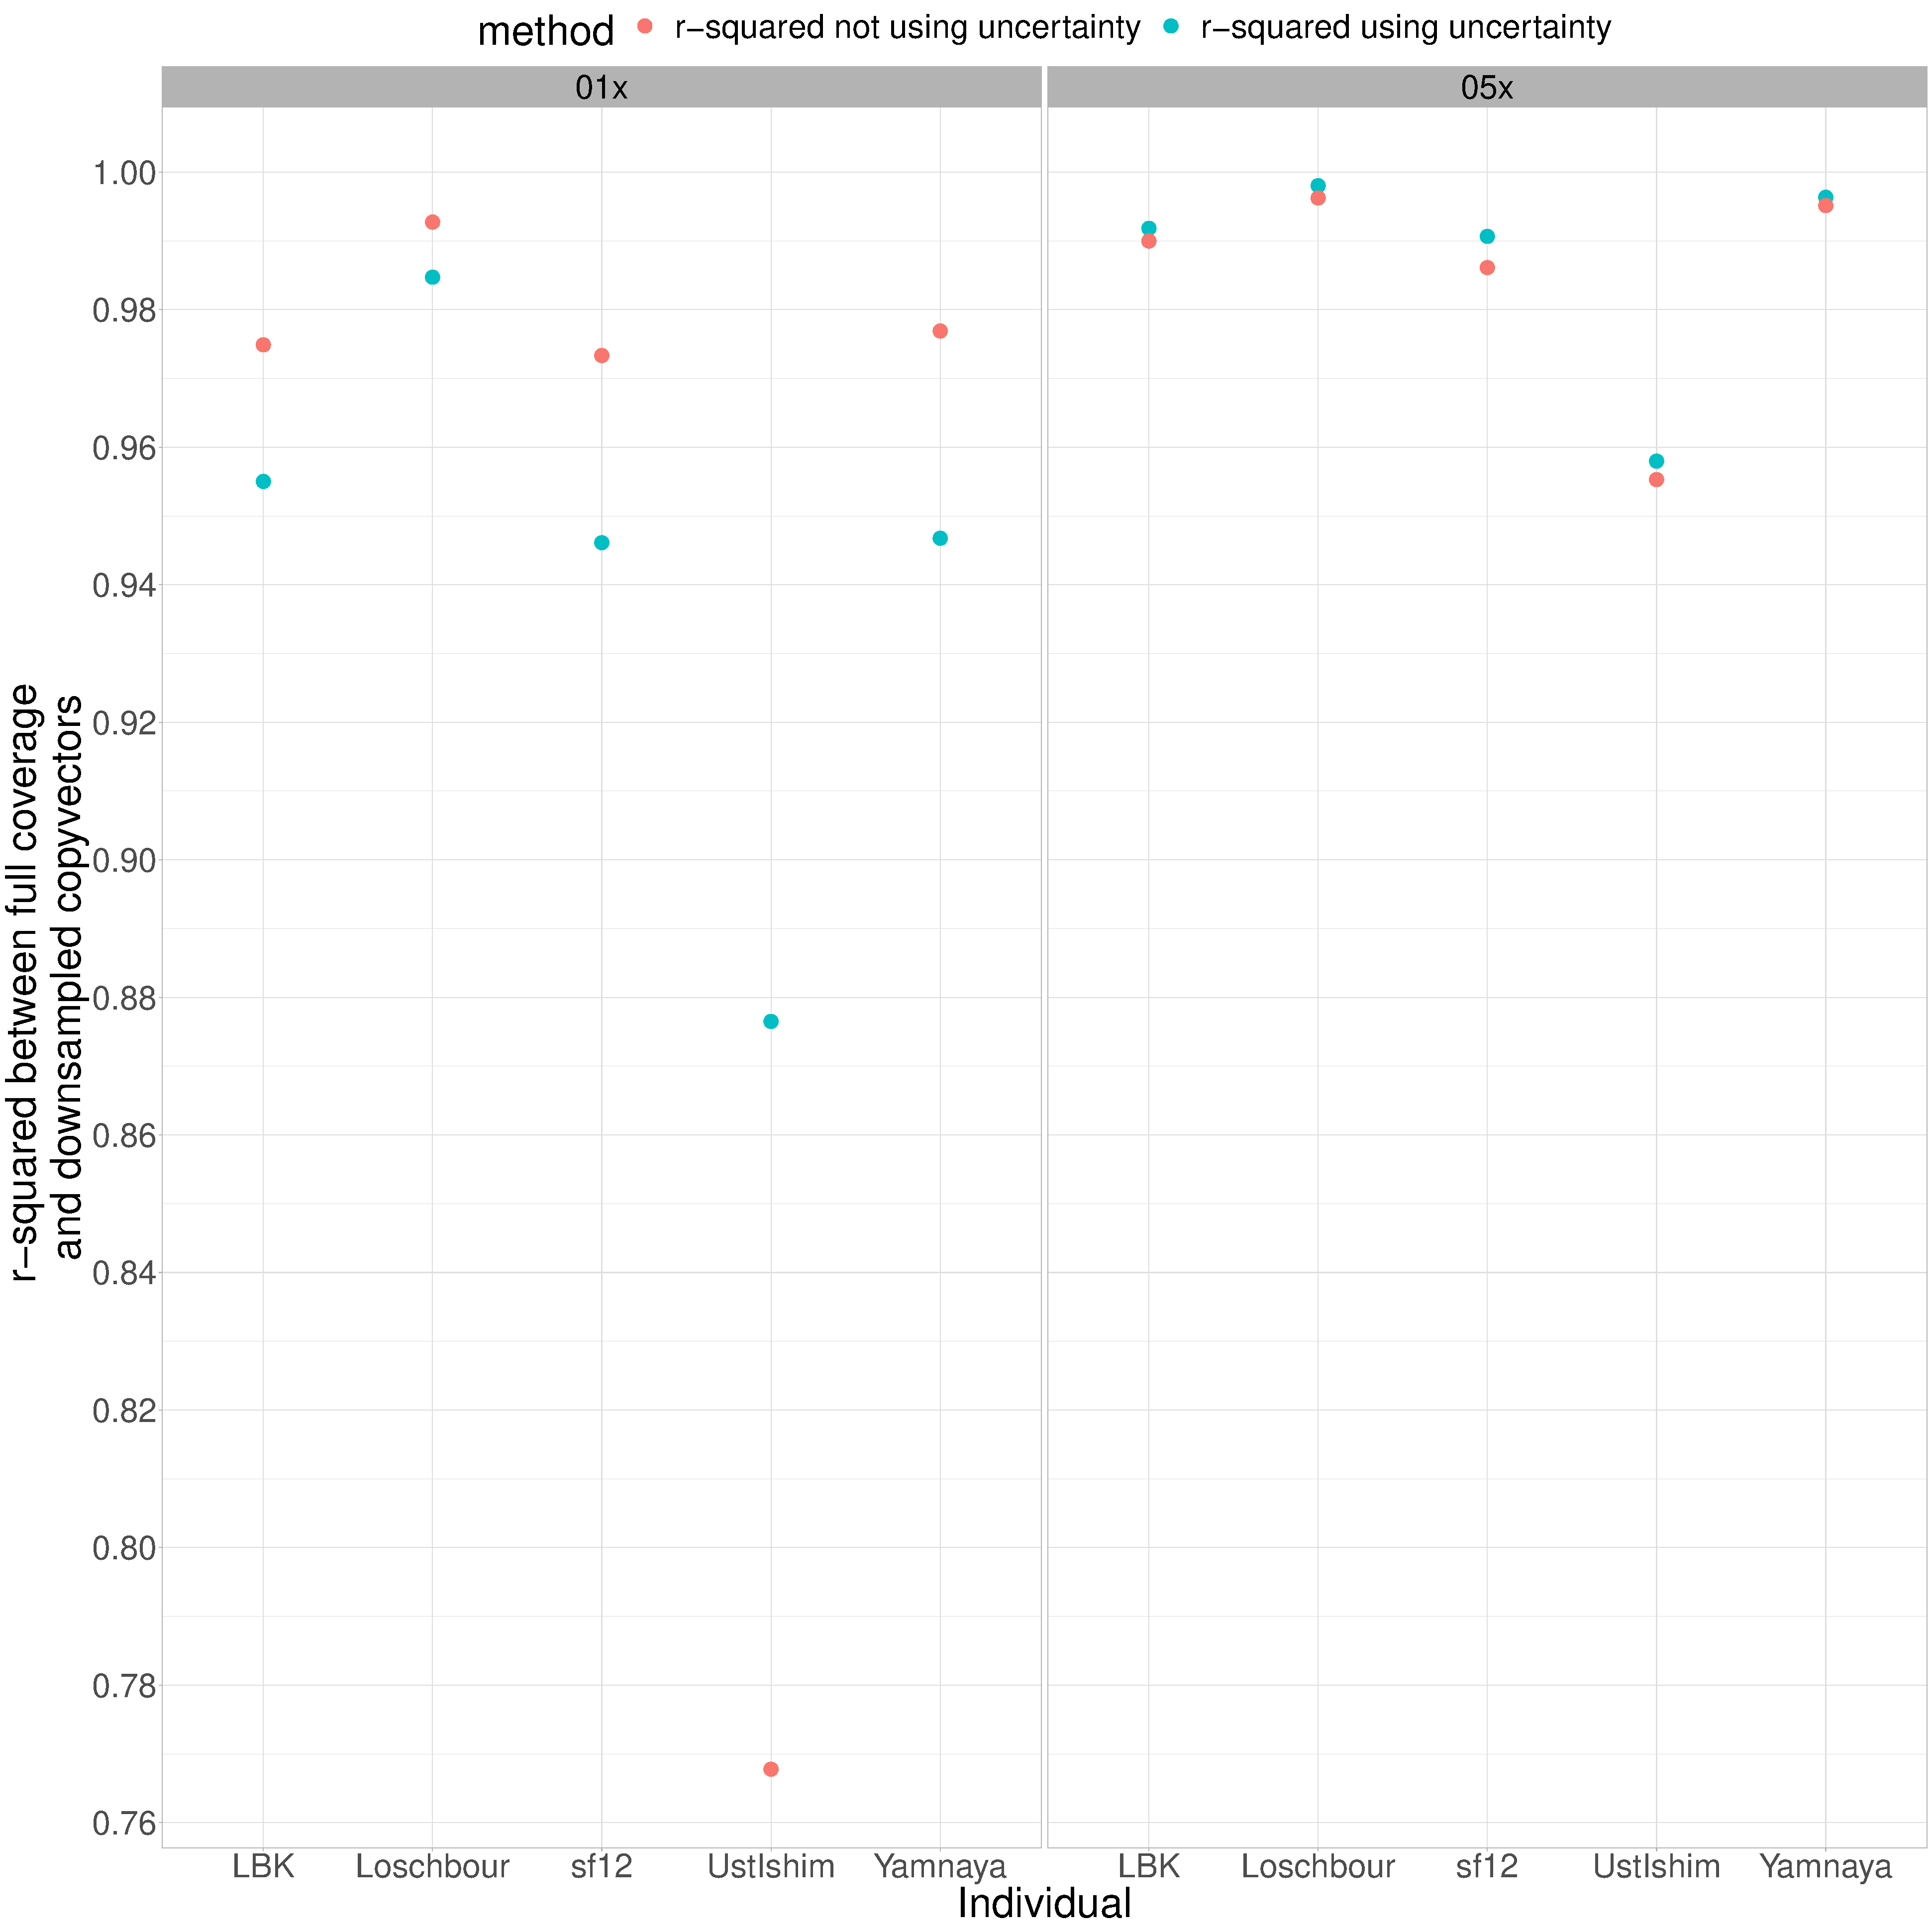
\includegraphics[width=1.0\textwidth]{../images/chapter1/uncertainty_v_noUncertainty_0.5x_0.1x.pdf}
    \caption{Comparison of performance of ChromoPainterV2 and ChromoPainterV2Uncertainty. Panels correspond to samples downsampled to 0.1x (left) and 0.5x (right). Points correspond to the r-squared between the downsampled individual and the same individual at full coverage. Red points are values obtained from ChromoPainterV2 and blue points are those obtained from ChromoPainterV2Uncertainty.}
    \label{fig:uncertainty_v_noUncertainty_0.5x_0.1x}
\end{figure}


\subsection{Filtering SNPs}

In this section, I will test whether filtering the set of input SNPs on different criteria reduces the effect of coverage related bias. 

The frequency of a particular variant in the reference panel (RAF - minor reference allele frequency) used for imputation is known to affect how accurately that variant can be imputed \cite{rubinacci2021efficient, delaneau2018integrative, Browning2016, hui2020evaluating}. Specifically, we expect variants which are less frequent in the reference panel to be imputed at a lower accuracy than those which are more frequent. Therefore, removing variants with a low frequency in the reference panel may mitigate the coverage related bias by removing variants which have been incorrectly imputed. In other words, we want to retain the SNPs where both alleles are relatively common within the population. 

For each individual, I took the 428,425 SNPs in the HellBus set and removed SNPs with $0.1 > RAF$ or $RAF > 0.9$, removing an average of 50,187 SNPs per individual. $RAF$ refers to the frequency of the allele in the 1000 genomes reference panel used to phase and impute the HellBus dataset. I then painted individuals downsampled to 0.1x and 0.5x using the standard set of 125 ancient donor individuals.  

Comparing the $TVD$ values between the copvyectors showed that this did not improve the 0.5x copyvectors (Table \ref{tab:TVD_table}). 

I then chose to filter SNPs based on $max(GP)$ at each position. $max(GP)$ correspond to the accuracy with which a SNP has been imputed, with higher values reflecting a higher chance of that genotype being imputed correctly. For each individual downsampled to 0.5x and 0.1x, I only retained positions where the $max(GP) >= 0.990$. For the 0.5x individuals, this resulted in a total of 348,852 SNPs for LBK, 339,949 for Loschbour, 315,075 for sf12, 308,961 for UstIshim and 386,484 for Yamnaya. Because different SNPs were removed from different individuals, each individual was painted separately. The same standard set of 124 ancient donors was used. Again, this did not improve the accuracy of the copyvectors. 


\begin{table}
\centering
\begin{tabular}[t]{lrrrrrrrr}
\toprule
sample & u\_01x & s\_01x & r\_01x & gp\_01x & u\_05x & s\_05x & r\_05x & gp\_05x\\
\midrule
LBK & 0.926 & 0.927 & 0.933 & 0.746 & 0.981 & 0.981 & 0.982 & 0.959\\
Loschbour & 0.898 & 0.898 & 0.907 & 0.654 & 0.980 & 0.980 & 0.976 & 0.925\\
sf12 & 0.923 & 0.923 & 0.942 & 0.774 & 0.981 & 0.981 & 0.980 & 0.950\\
UstIshim & 0.944 & 0.944 & 0.945 & 0.827 & 0.980 & 0.980 & 0.976 & 0.960\\
Yamnaya & 0.915 & 0.915 & 0.920 & 0.726 & 0.986 & 0.986 & 0.985 & 0.964\\
\bottomrule
\end{tabular}
\caption{Table of $1-TVD$ values between the copyvectors of full coverage and downsampled individuals. `u' refers to ChromoPainterUncertainty, `s' refers to ChromoPainterV2, `r' refers to filtering SNPs with reference allele frequency (RAF) $0.1 > RAF$ or $RAF > 0.9$ and `gp' refers to filtering by $max(GP) >= 0.990$.}
\label{tab:TVD_table}
\end{table}


\subsection{Restricting analysis to non-imputed SNPs}

Section \ref{sec:PCAImputationTest} showed that imputation was the likely cause of coverage related bias. Thus, restricting ChromoPainter analysis to non-imputed SNPs above a certain coverage may mitigate such bias.

However, removing SNPs may have negative side-effects; increasing the genetic distance between SNPs reduces linkage information and therefore may reduce the overall power to distinguish between closely related haplotypes. At the most extreme case, retaining only a small number of SNPs may effectively reduce the method to unlinked and lose the advantage given by accounting for haplotypes. This may be important if we decide to restrict analysis to non-imputed SNPs, as low coverage samples may only have a small number of high enough coverage, non-imputed SNPs. Therefore, it is important to determine whether samples of a particular coverage have enough regions containing enough high-coverage SNPs to retain the advantages of haplotype-based methods over unlinked ones. 

One case study to test whether a set of SNPs has enough linkage information is to determine whether it is possible to distinguish individuals born in Devon from those born in Cornwall. This has shown to be possible using the fineSTRUCTURE clustering algorithm using linkage information, but not using unlinked methods (ADMIXTURE \cite{alexander2009fast}) \cite{Leslie2015}. Therefore, determining whether it is possible to distinguish between individuals from Devon and Cornwall acts as a test case for determining how many high-coverage SNPs would give sufficient SNP density to distinguish between these two populations.

To assess this, I painted individuals from Devon (n=73) and Cornwall (n=89) with all other POBI individuals as donors (n=2,039), using the full set of SNPs (n=452,592). It is necessary to develop a classification score which quantifies to what degree it is possible to distinguish between individuals from Devon and Cornwall. For a classification score, I calculated the proportion of Cornwall individuals whose copy vector had a lower $TVD$ with the mean copyvector of all other Cornwall individuals than with the mean copy vector of all Devon individuals. In other words, this asks whether the individual is genetically closer to the Devon or Cornwall population.

I repeated the analogous procedure to find a classification score for Devon individuals, given in table \ref{tab:prob_assignment_DevCorn}. I then painted the same individuals using a reduced set of SNPs, in particular reducing the set of SNPs to 12 different percentages ranging from 0.2\% - 90\% of the total original number of SNPs (a full list of the reduction levels and details of the painting procedure can be found in the methods section \ref{sec:ReducingSNPcount}). Painting using a reduced set of SNPs is intended to simulate an ancient genome where only a subset of the total number of SNPs have been covered by a sufficient number of reads. Defining `sufficient' isn't precisely defined, but it is possible to calculate the probability of observing both reads given $x$ reads at a given heterozygous positions and assuming equal probability of observing reference and non-reference alleles; for example, 9 reads are needed to obtain at least a 0.995 probability of observing both alleles (Fig. \ref{fig:ProbabilityHetReads}).

\begin{figure}[htp]
    \centering
    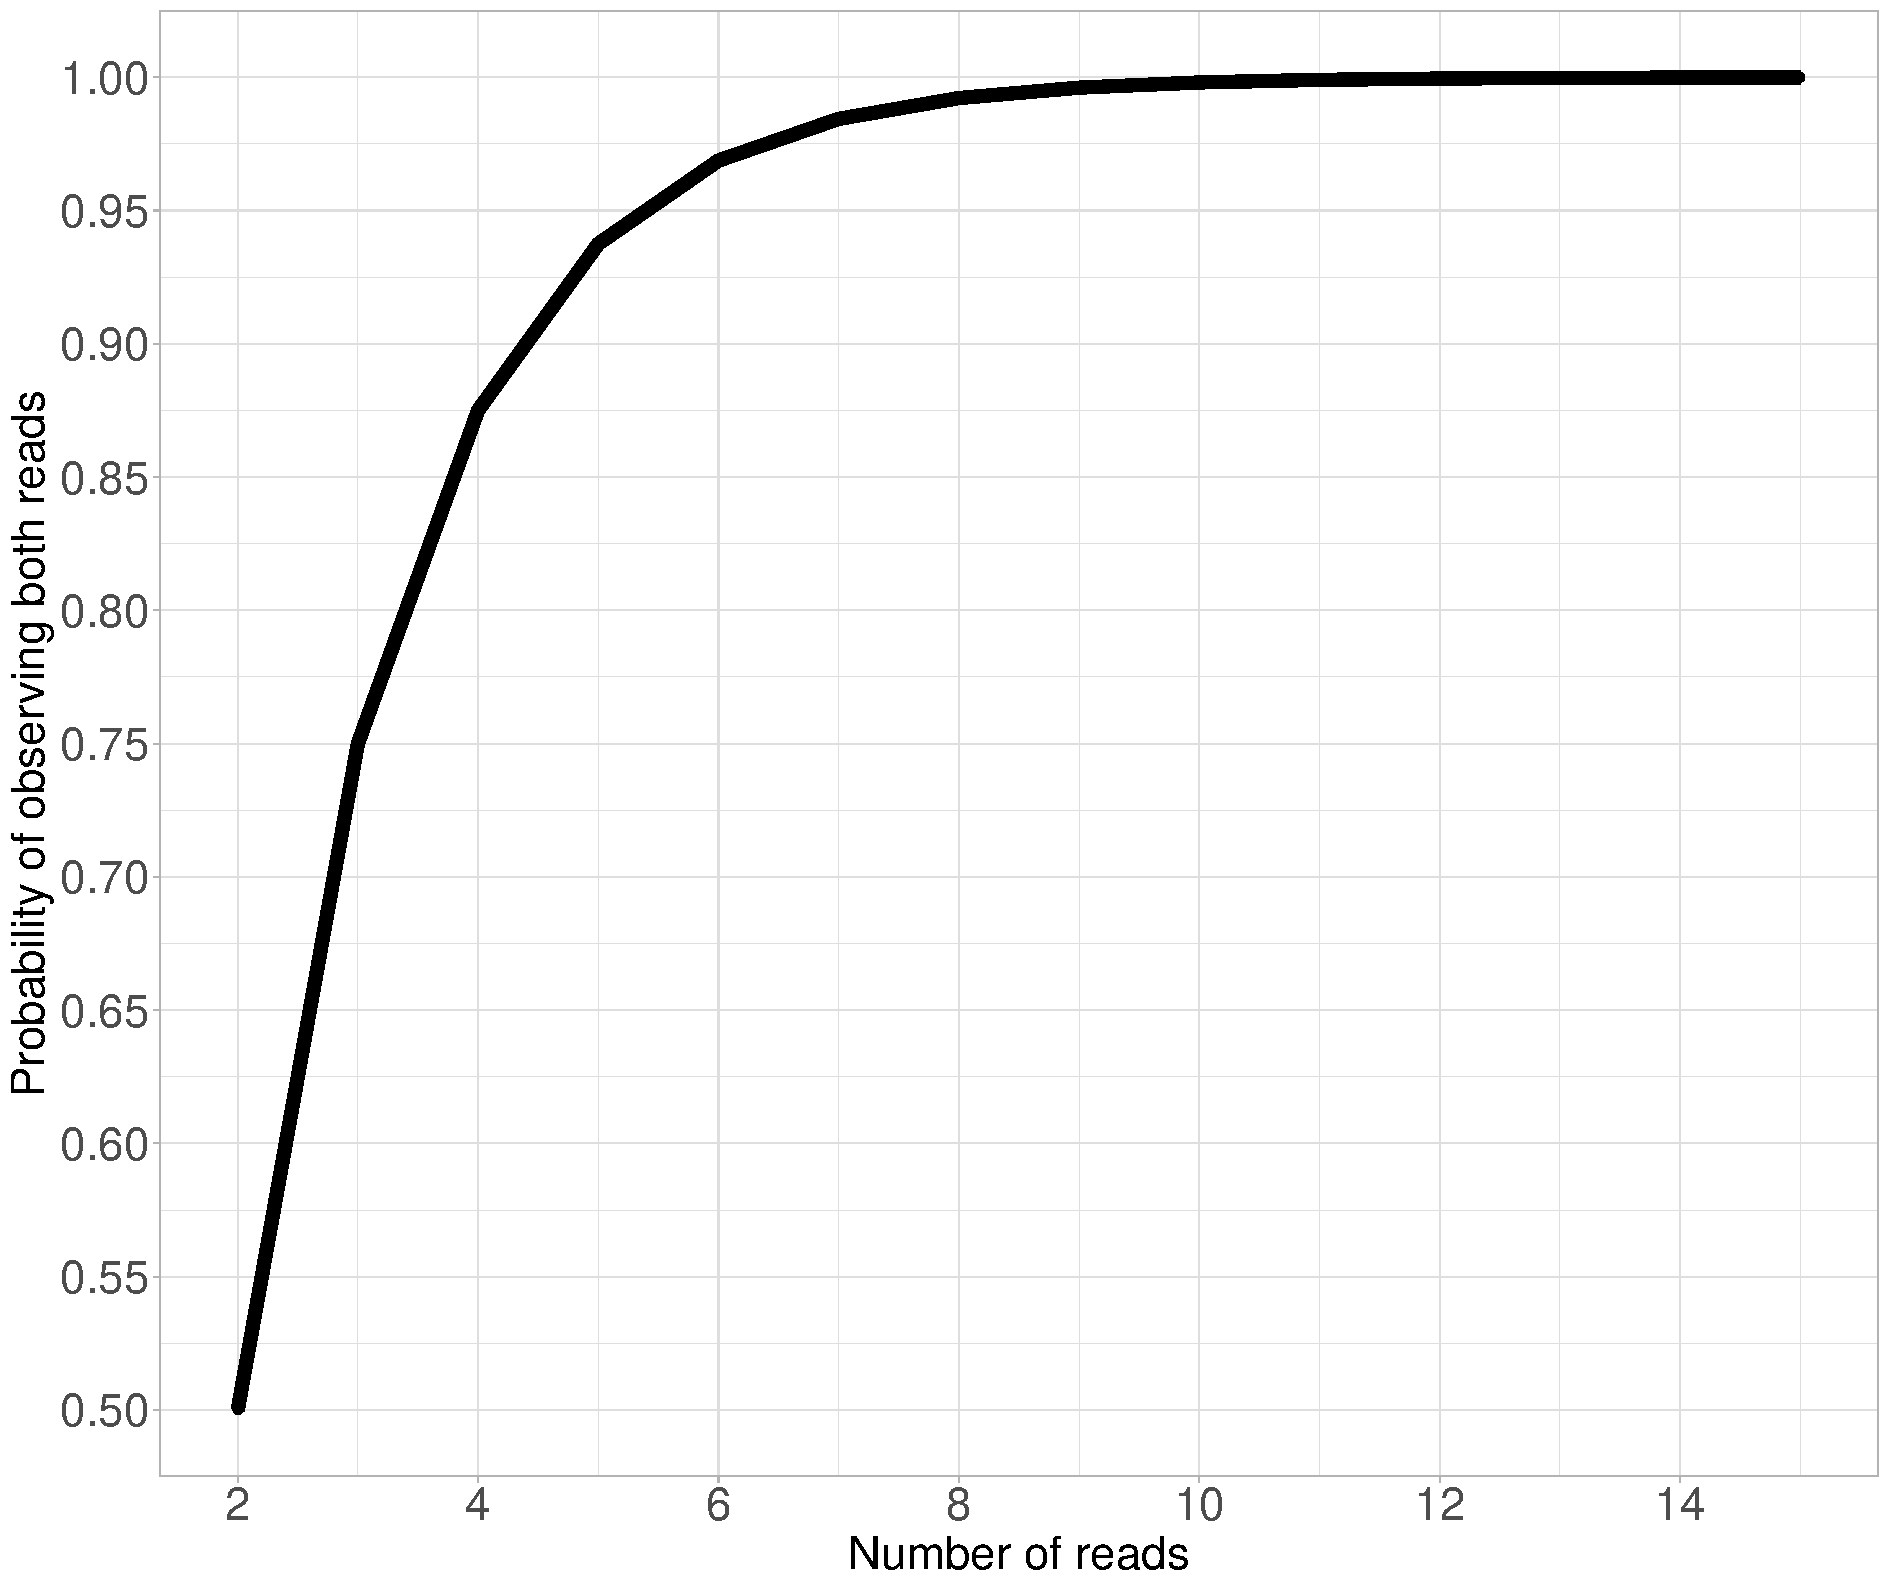
\includegraphics[width=1.0\textwidth]{../images/chapter1/het_prob.pdf}
    \caption{Probability of observing both reads at a heterozygous positions, given $x$ reads assuming equal probability of observing reference and non-reference alleles.}
    \label{fig:ProbabilityHetReads}
\end{figure}


\begin{table}
\centering
\begin{tabular}[t]{crr}
\toprule
\thead{Percentage \\ of SNPs retained} & Cornwall & Devon\\
\midrule
1 \% & 0.801 & 0.945\\
2 \% & 0.820 & 0.986\\
3 \% & 0.876 & 0.973\\
4 \% & 0.910 & 0.973\\
5 \% & 0.888 & 0.973\\
6 \% & 0.899 & 0.973\\
7 \% & 0.888 & 0.973\\
8 \% & 0.910 & 0.973\\
9 \% & 0.910 & 0.973\\
10 \% & 0.910 & 0.973\\
20 \% & 0.921 & 0.973\\
30 \% & 0.910 & 0.973\\
40 \% & 0.899 & 0.973\\
50 \% & 0.910 & 0.973\\
70 \% & 0.910 & 0.973\\
80 \% & 0.910 & 0.973\\
90 \% & 0.921 & 0.973\\
\bottomrule
\end{tabular}
\caption{Proportion of individuals correctly assigned to their population at different percentages of SNPs retained.}
\label{tab:prob_assignment_DevCorn}
\end{table}


In my painting of 5998 world-wide samples on the Human Origins array (described in Appendix section \ref{HumanOriginsAppendix}), the average number of segments that forms a recipient genome is 9764 (range: 1437-18,963). Given a genome-wide size of $\approx$ 3000Mb, this implies that an average `chunk' size (in Mb) is 3000/9764 = 307.2 $\approx$ 500kb, where a `chunk' is a set of contiguous SNPs matched to a single donor. Therefore, for each of the 12 different levels of SNP reduction used in my Devon/Cornwall analysis, I can calculate the average number of SNPs per 500kb chunks, and determine how many of these 500kb chunks are necessary to accurately distinguish individuals from Devon and Cornwall. To do so, for each reduced SNP percentage, I found the Cornwall/Devon classification score using only data from chromosome 22 (which has only W 500kb chunks), and using only chromosomes 21 and 22 (which has V 500Kb chunks), etc, continuing until the classification scores were equivalent to that when analysing all 22 autosomes at all 452,592 SNPs. In this way, for each reduced SNP percentage, I found the number of 500Kb chunks necessary to as accurately distinguish between Devon and Cornwall as in the case where we had analysed a full data set of 452,592 SNPs (Table \ref{table:windows_power_table_DevCorn}). I found results to be very similar to if chunk-size were instead defined as 250kb or 1Mb (Table \ref{table:windows_power_table_DevCorn}).


I repeated an identical analysis, including reducing the total number of SNPS, using individuals from the Mandenka and Yoruba ethnic groups rather than Devon and Cornwall.  

\begin{table}[!h]
\centering
\begin{tabular}[t]{lrrrc}
\toprule
\thead{Number of SNPs\\ retained} & 250Kb & 500Kb & 1Mb & \thead{Number of\\ SNPs per 500Kb \\Window}\\
\midrule
20,000 & 9356 & 4715 & 2388 & 3.3\\
25,000 & 6954 & 3509 & 1781 & 4.1\\
30,000 & 6272 & 3166 & 1607 & 5.0\\
35,000 & 4083 & 2064 & 1049 & 5.8\\
40,000 & 3099 & 1565 & 796 & 6.6\\
45,000 & 3602 & 1820 & 925 & 7.5\\
50,000 & 2612 & 1321 & 673 & 8.3\\
100,000 & 1304 & 661 & 338 & 16.6\\
150,000 & 1005 & 508 & 260 & 25.0\\
200,000 & 705 & 357 & 183 & 33.3\\
250,000 & 705 & 357 & 183 & 41.6\\
300,000 & 506 & 255 & 130 & 50.0\\
350,000 & 267 & 135 & 69 & 58.3\\
400,000 & 705 & 357 & 183 & 66.6\\
450,000 & 136 & 69 & 35 & 75.0\\
\bottomrule
\end{tabular}
\caption{Number of 250Kb, 500Kb or 1Mb windows required at different levels of SNP reduction to match the TVD assignment power of 500K fully genotyped SNPs for individuals in Devon and Cornwall. Note that the number of necessary 250kb and 500kb windows is roughly four and two times, respectively, the number of 1Mb windows, indicating the definition of window size makes little difference.}
\label{table:windows_power_table_DevCorn}
\end{table}

\begin{table}
\centering
\begin{tabular}[t]{lrrrr}
\toprule
\thead{Number of SNPs\\ retained} & 250Kb & 500Kb & 1Mb & \thead{Number of\\ SNPs per 500Kb \\Window}\\
\midrule
30,000 & 6272 & 3166 & 1607 & 5.0\\
35,000 & 3099 & 1565 & 796 & 5.8\\
40,000 & 3099 & 1565 & 796 & 6.6\\
45,000 & 2612 & 1321 & 673 & 7.5\\
50,000 & 3099 & 1565 & 796 & 8.3\\
100,000 & 1886 & 956 & 489 & 16.6\\
150,000 & 1304 & 661 & 338 & 25.0\\
200,000 & 506 & 255 & 130 & 33.3\\
250,000 & 267 & 135 & 69 & 41.6\\
300,000 & 506 & 255 & 130 & 50.0\\
350,000 & 506 & 255 & 130 & 58.3\\
400,000 & 506 & 255 & 130 & 66.6\\
450,000 & 267 & 135 & 69 & 75.0\\
\bottomrule
\end{tabular}
\caption{Number of 250Kb, 500Kb or 1Mb windows required at different levels of SNP reduction to match the TVD assignment power of 500K fully genotyped SNPs for individuals in from Mandenka and Yoruba ethnic groups.}
\label{table:windows_power_table_ManYor}
\end{table}

Guided by these results, for each ancient individual (n=587, median coverage=1.1x), I found the number of non-overlapping windows of sizes 250Kb, 500Kb or 1Mb that had $Y$ SNPs above $Z$ coverage, varying both Y and Z. 

Fig \ref{fig:avg_good_windows} shows the mean number of 500Kb windows per individual with at least $Y$ SNPs above $Z$ coverage, with individuals grouped into bins based on their mean coverage. Points are coloured yellow if, within the bin of coverage, samples have at least 2000 windows.

Samples less than 0.5x do not have enough windows, even if the threshold for a `good' SNPs is being covered by a single read. As is it not possible to call a heterozygous position with only a single read, this suggests that there are not enough non-imputed SNPs with enough coverage to match the power seen in full coverage individuals. For example, samples between 0.3-0.4x have approximately 1000 segments with $\geq$ 10 SNPs above 2x in coverage; Table \ref{table:windows_power_table_DevCorn} shows that 1565 windows of $\geq$ 8.3 SNPs is enough to match full power. However, as Figure \ref{fig:ProbabilityHetReads} shows, 50\% of these genotypes may not observe both reads if the position is heterozygous. Indeed, even when there are 3 reads covering a site, there is still a 25\% chance of not identifying a heterozygous position. Only the samples in the 2-5x coverage bin had enough windows when using a coverage threshold of 4 and 5 reads. 

This analysis therefore suggests that there are not enough regions with enough high quality SNPs at mean coverages less than 2x to reliably analyse using ChromoPainter.

\begin{figure}[htp]
    \centering
    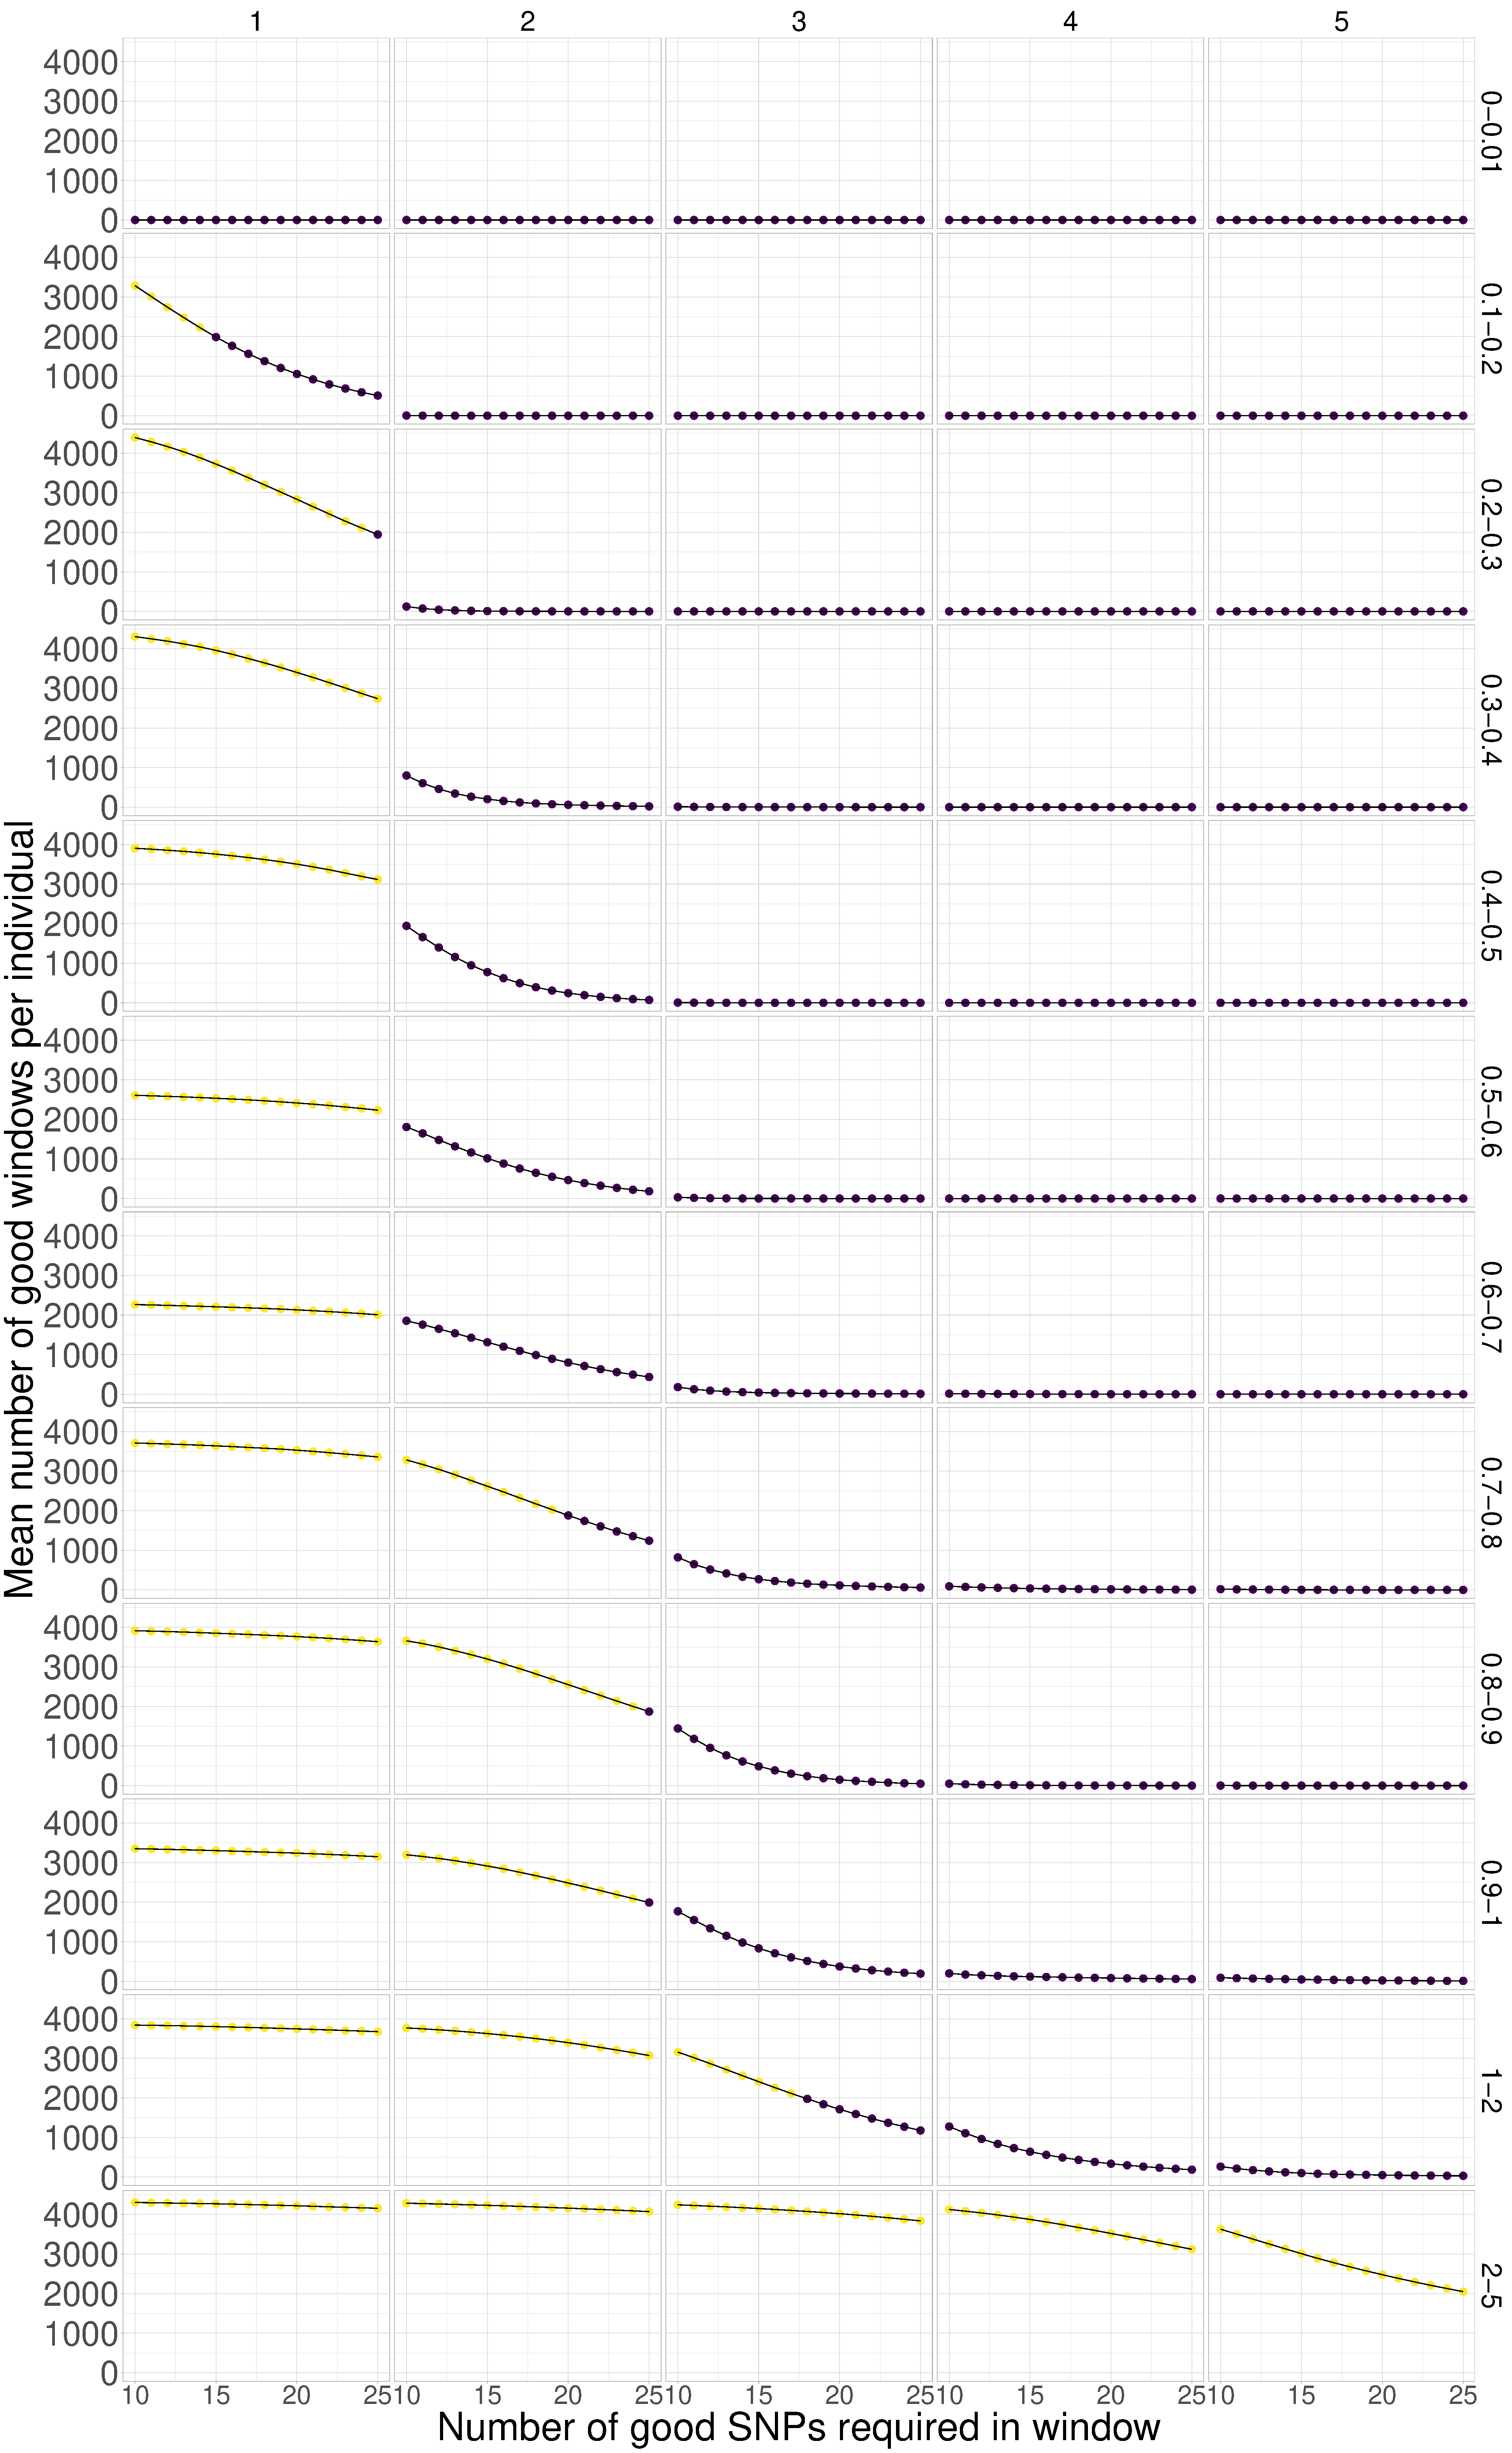
\includegraphics[width=1.0\textwidth]{../images/chapter1/avg_good_windows.pdf}
    \caption{Mean number of 500Kb windows (y-axis) within the genome of each ancient individuals within a given range of coverages (rows) with at least $Y$ SNPs (x-axis) above a particular coverage $Z$ (columns)}
    \label{fig:avg_good_windows}
\end{figure}


\begin{figure}[htp]
    \centering
    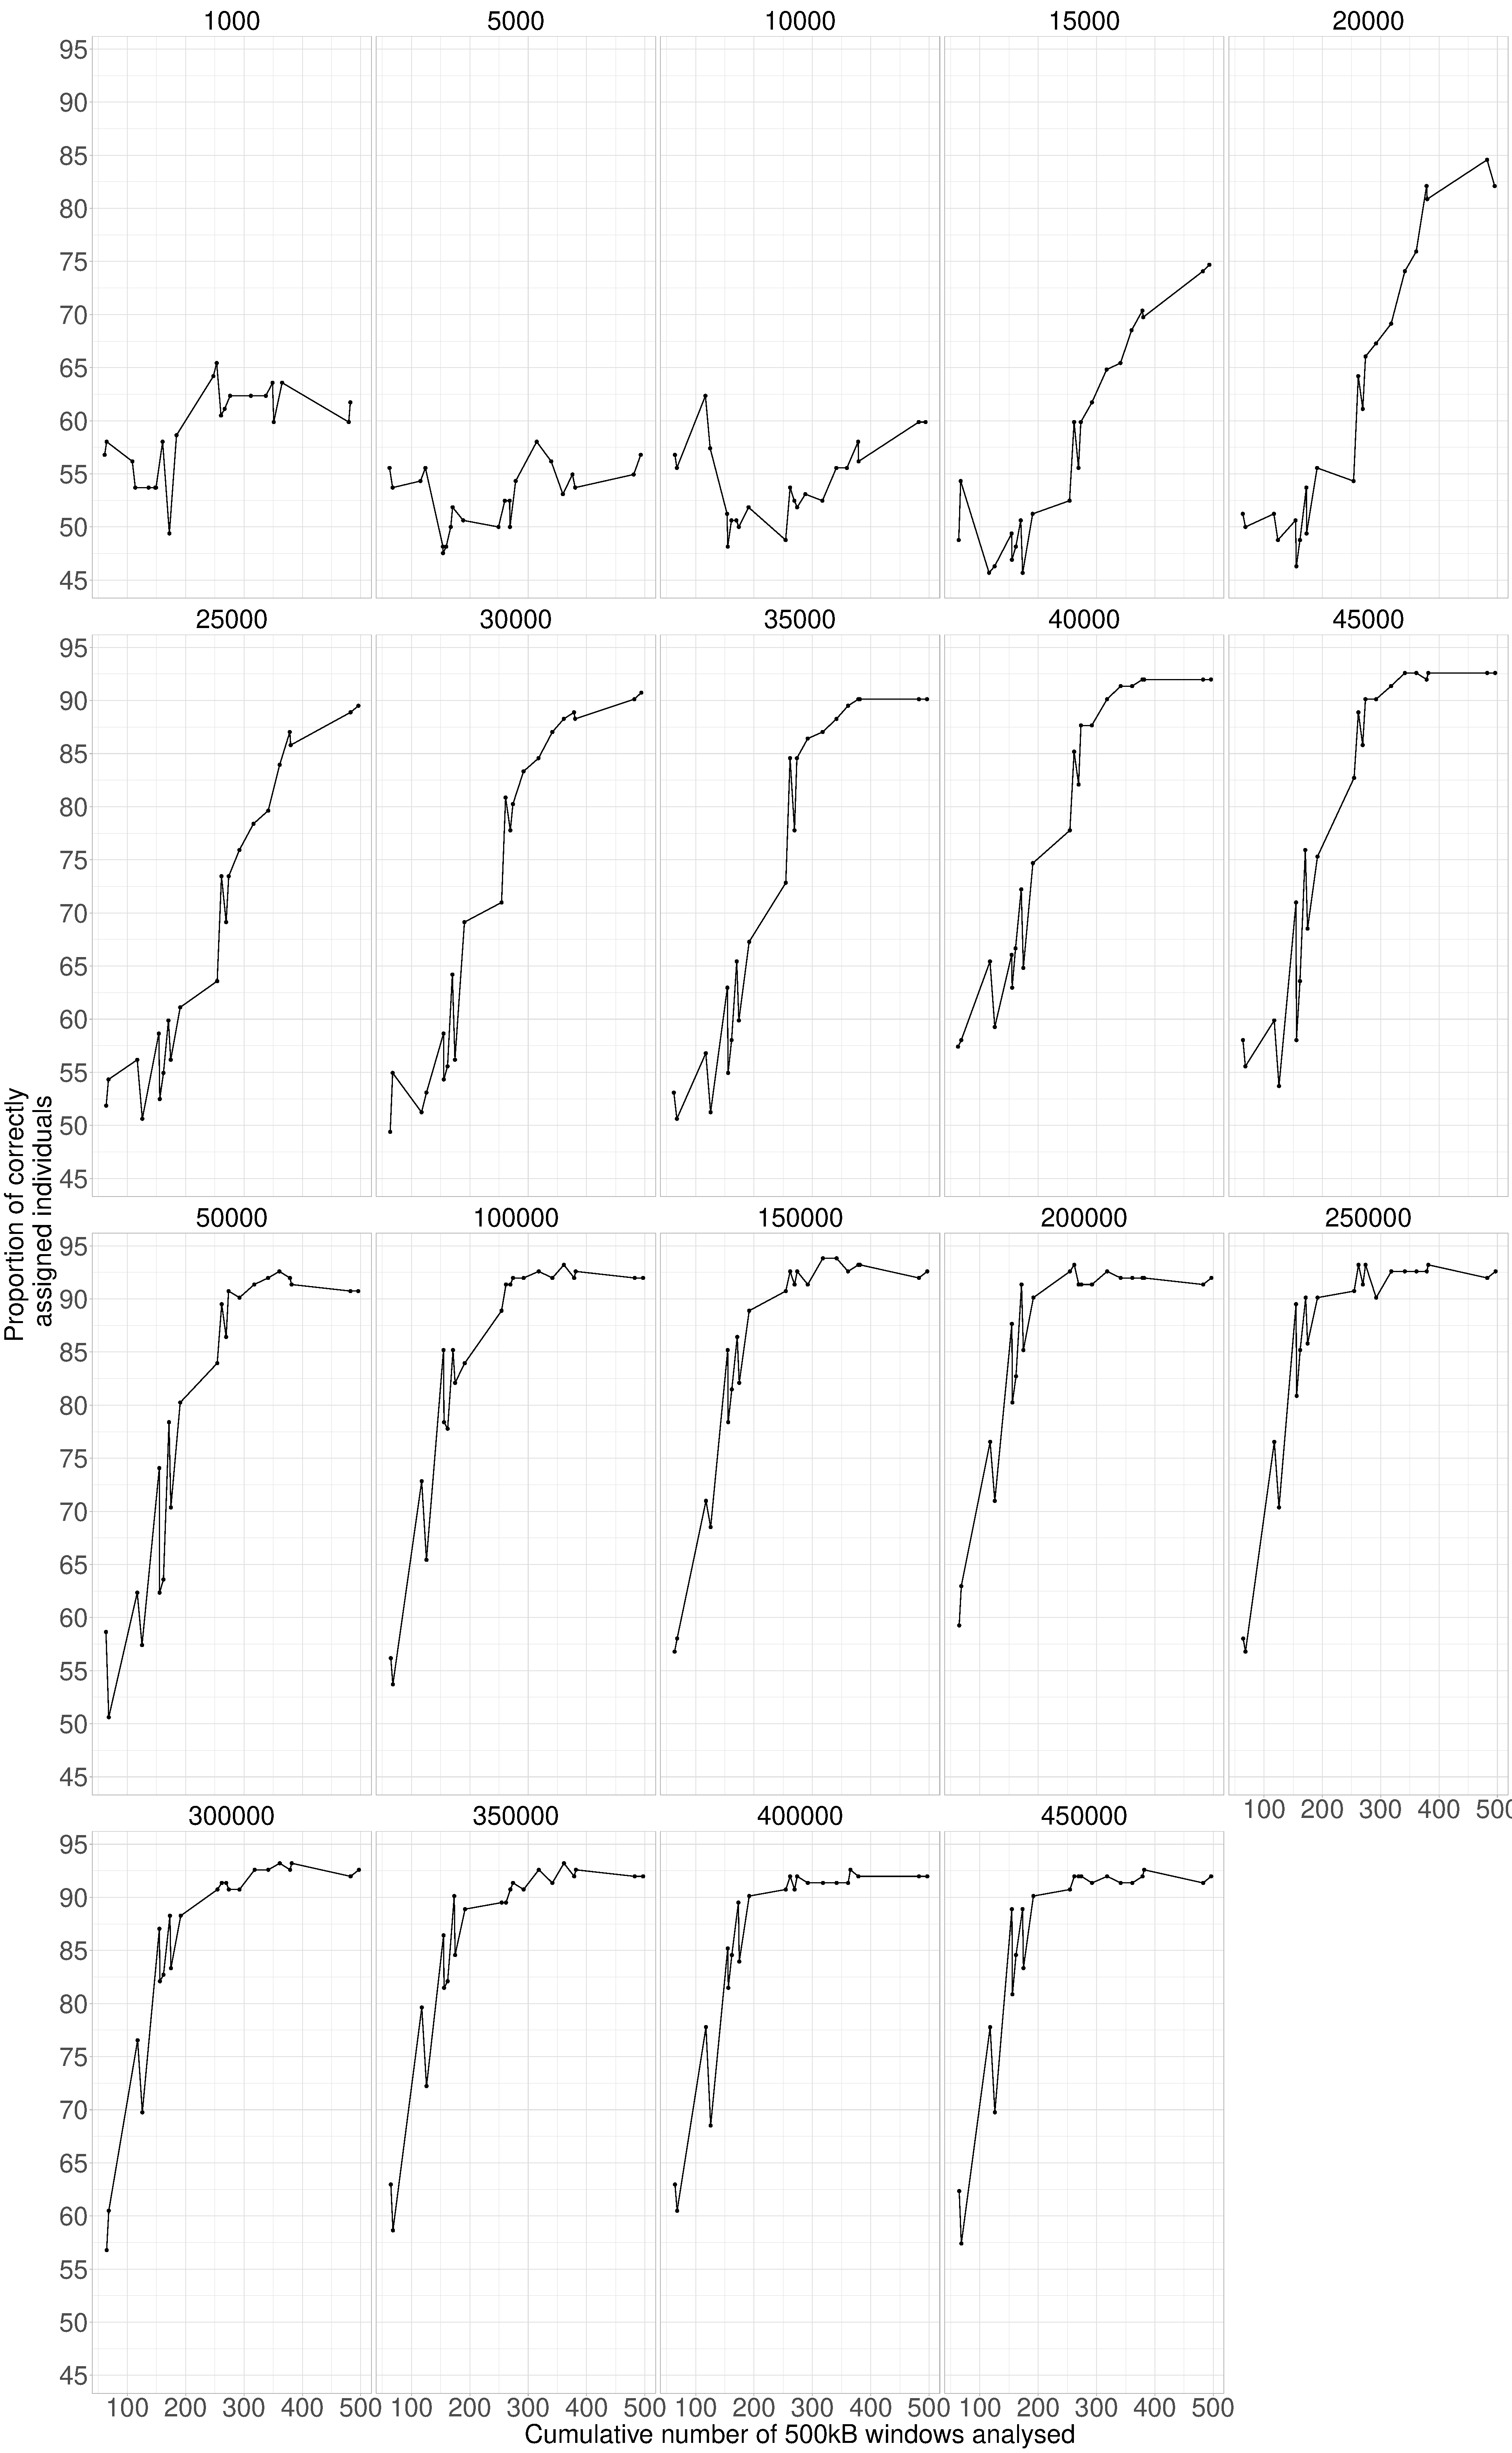
\includegraphics[width=1.0\textwidth]{../images/chapter1/cumulative_windows_val.pdf}
    \caption{The effect of adding 500kB windows on the ability to assign individuals from Devon and Cornwall to their respective populations. Each panel represents a different total number of SNPs used. X-axis gives the cumulative number of 500kB windows used in analysis. Y-axis gives the combined proportion of individuals assigned.}
    \label{fig:cumulative_windows_val}
\end{figure}


\section{Summary of Results and Discussion}

In this section I used a downsampling approach on five high-coverage ancient DNA samples to show that ChromoPainter analysis can be performed on samples down to 0.5x coverage without showing a significant deviation from the same sample at full coverage. In particular, ChromoPainter copyvectors, SOURCEFIND ancestry proportion estimates and Principle Component Analysis position all of 0.5x coverage and higher showed a good correspondence with the same metrics at full coverage. The 0.1x downsampled showed deviations from the full coverage samples which meant that they cannot currently be analysed reliably with ChromoPainter and its associated methods. I showed that imputation introduces bias into low-coverage samples that is manifested by those samples being shifted towards the centre of a PCA. 

I performed a range of analyses to try and recover useful haplotype information from low coverage samples and improve the performance of the analysis. Counter-intuitively, approaches such as removing SNPs with a low imputation quality and reference allele frequency did not improve the performance of ChromoPainter on low coverage samples. However, this is broadly consistent with a single previous study, which also showed that filtering the dataset for SNPs with a low imputation quality score did not substantially affect fineSTRUCTURE clustering \cite{Martiniano2017}. However, it also runs counter to studies which have shown filtering SNPs based on imputation quality score can significantly reduce the number of incorrectly imputed genotypes \cite{hui2020evaluating}. 

I also developed a modification to the ChromoPainter model which accounted for uncertainty in genotype calls; however it only marginally improved the performance of ChromoPainter on samples of 0.5x or higher. Again, this was surprising, as previously published methodology which accounts for genotype likelihoods when estimating IBD tracts has been shown to be effective \cite{Vieira2016}.

Finally, I used simulated data from present-day individuals to show that samples around 0.5x coverage can in theory be analysed with useful haplotype information, but that imputation is necessary for lower coverage samples.

Many of the analyses performed in this section only used a single target sample, as I did not identify a way to generate multiple downsampled individuals from the same population. For example, the SOURCEFIND analysis I performed  used a single target downsample when estimating ancestry proportions. This differs from a typical ancient DNA analysis, such as those of Margaryan et al \cite{margaryan2020population}, where there may be up to 20 low coverage samples per population. This number may increase in the future as the technology to generate ancient DNA improves. Leveraging information across multiple samples from the same population  would improve the accuracy of population-wide ancestry or admixture estimates, for example. Thus, the results presented in this section which used a single target individual may underestimate the ability to analyse low-coverage samples. It may be possible to accurately analyse 0.1x samples if there are multiple samples per population. 

In this section I used present-day individuals to estimate the number and size of chunks needed to retain haplotype information. This was because present-day individuals are simpler to analyse; the populations are better defined than in ancient samples (i.e. it is possible to only include individuals whose grandparents were born within 100kM of a target location), are of uniform coverage and contain many more individuals per population. Thus, using present-day individuals removes potentially confounding factors that may be present when analysing ancient samples. However, using present-day samples to draw conclusions about ancient samples may lead to underestimating the number of SNPs per window required. As the present-day samples had been genotyped high-quality DNA samples and a genotpying array, each genotype can be called with a high confidence. This is not the case with ancient samples, where each SNP may be covered by a small number (<3) of reads.

For the imputation and phasing reference panel, I used the 1000 genomes dataset which contains around 6000 haplotypes. The Haplotype Reference Consortium contains roughly 10 times as many haplotypes and thus offers substantial gains in the potential accuracy of genotype imputation \cite{rubinacci2021efficient}. I did not use the HRC owing to difficulties in obtaining access to the data; however, I expect that future studies which use this resource will be able to analyse ancient DNA samples of low coverage to a higher degree of accuracy. 

Whilst I did not interrogate the range of coverages between 0.1-0.5x, this could be an avenue for future research.



